%%%%%%%%%%%%%%%%%%%%%%%%%%%%%%%%%%%%%%%%%
% Masters/Doctoral Thesis 
% LaTeX Template
% Version 1.43 (17/5/14)
%
% This template has been downloaded from:
% http://www.LaTeXTemplates.com
%
% Original authors:
% Steven Gunn 
% http://users.ecs.soton.ac.uk/srg/softwaretools/document/templates/
% and
% Sunil Patel
% http://www.sunilpatel.co.uk/thesis-template/
%
% License:
% CC BY-NC-SA 3.0 (http://creativecommons.org/licenses/by-nc-sa/3.0/)
%
% Note:
% Make sure to edit document variables in the Thesis.cls file
%
%%%%%%%%%%%%%%%%%%%%%%%%%%%%%%%%%%%%%%%%%

%----------------------------------------------------------------------------------------
%	PACKAGES AND OTHER DOCUMENT CONFIGURATIONS
%----------------------------------------------------------------------------------------

\documentclass[11pt, oneside]{Thesis} % The default font size and one-sided printing (no margin offsets)

\graphicspath{{Pictures/}} % Specifies the directory where pictures are stored

\usepackage[square, numbers, comma, sort&compress]{natbib} % Use the natbib reference package - read up on this to edit the reference style; if you want text (e.g. Smith et al., 2012) for the in-text references (instead of numbers), remove 'numbers' 
\usepackage{listings,alltt}
\lstset{language=bash}
\usepackage{color}
\hypersetup{urlcolor=blue, colorlinks=true} % Colors hyperlinks in blue - change to black if annoying
\title{\ttitle} % Defines the thesis title - don't touch this

\begin{document}

\frontmatter % Use roman page numbering style (i, ii, iii, iv...) for the pre-content pages

\setstretch{1.3} % Line spacing of 1.3

% Define the page headers using the FancyHdr package and set up for one-sided printing
\fancyhead{} % Clears all page headers and footers
\rhead{\thepage} % Sets the right side header to show the page number
\lhead{} % Clears the left side page header

\pagestyle{fancy} % Finally, use the "fancy" page style to implement the FancyHdr headers

\newcommand{\HRule}{\rule{\linewidth}{0.5mm}} % New command to make the lines in the title page

% PDF meta-data
\hypersetup{pdftitle={\ttitle}}
\hypersetup{pdfsubject=\subjectname}
\hypersetup{pdfauthor=\authornames}
\hypersetup{pdfkeywords=\keywordnames}
% ADDED BY MAGNUS 

%----------------------------------------------------------------------------------------
%	TITLE PAGE
%----------------------------------------------------------------------------------------

\begin{titlepage}
\begin{center}

\textsc{\LARGE \univname}\\[1.5cm] % University name
\textsc{\Large Project TMA4500}\\[0.5cm] % Thesis type

\HRule \\[0.4cm] % Horizontal line
{\huge \bfseries \ttitle}\\[0.4cm] % Thesis title
\HRule \\[1.5cm] % Horizontal line
 
\begin{minipage}{0.4\textwidth}
\begin{flushleft} \large
\emph{Author:}\\
\href{http://www.johnsmith.com}{\authornames} % Author name - remove the \href bracket to remove the link
\end{flushleft}
\end{minipage}
\begin{minipage}{0.4\textwidth}
\begin{flushright} \large
\emph{Supervisor:} \\
\href{http://www.jamessmith.com}{\supname} % Supervisor name - remove the \href bracket to remove the link  
\end{flushright}
\end{minipage}\\[3cm]
 
%\large \textit{A thesis submitted in fulfilment of the requirements\\ for the degree of \degreename}\\[0.3cm] % University requirement text
%\textit{in the}\\[0.4cm]
\groupname\\\deptname\\[2cm] % Research group name and department name
 
{\large \today}\\[4cm] % Date
%\includegraphics{Logo} % University/department logo - uncomment to place it
 
\vfill
\end{center}

\end{titlepage}
%%fakesection - Declaration of Authorship
%----------------------------------------------------------------------------------------
%	DECLARATION PAGE
%	Your institution may give you a different text to place here
%----------------------------------------------------------------------------------------
%\Declaration{

%\addtocontents{toc}{\vspace{1em}} % Add a gap in the Contents, for aesthetics

%I, \authornames, declare that this thesis titled, '\ttitle' and the work presented in it are my own. I confirm that:

%\begin{itemize} 
%\item[\tiny{$\blacksquare$}] This work was done wholly or mainly while in candidature for a research degree at this University.
%\item[\tiny{$\blacksquare$}] Where any part of this thesis has previously been submitted for a degree or any other qualification at this University or any other institution, this has been clearly stated.
%\item[\tiny{$\blacksquare$}] Where I have consulted the published work of others, this is always clearly attributed.
%\item[\tiny{$\blacksquare$}] Where I have quoted from the work of others, the source is always given. With the exception of such quotations, this thesis is entirely my own work.
%\item[\tiny{$\blacksquare$}] I have acknowledged all main sources of help.
%\item[\tiny{$\blacksquare$}] Where the thesis is based on work done by myself jointly with others, I have made clear exactly what was done by others and what I have contributed myself.\\
%\end{itemize}
 
%Signed:\\
%\rule[1em]{25em}{0.5pt} % This prints a line for the signature
 
%Date:\\
%\rule[1em]{25em}{0.5pt} % This prints a line to write the date
%}

%\clearpage % Start a new page
%%fakesection - Quotation page
%----------------------------------------------------------------------------------------
%	QUOTATION PAGE
%----------------------------------------------------------------------------------------

%\pagestyle{empty} % No headers or footers for the following pages

%\null\vfill % Add some space to move the quote down the page a bit

%\textit{``Thanks to my solid academic training, today I can write hundreds of words on virtually any topic without possessing a shred of information, which is how I got a good job in journalism."}

%\begin{flushright}
%Dave Barry
%\end{flushright}

%\vfill\vfill\vfill\vfill\vfill\vfill\null % Add some space at the bottom to position the quote just right

%\clearpage % Start a new page

%----------------------------------------------------------------------------------------
%	ABSTRACT PAGE
%----------------------------------------------------------------------------------------
%%fakesection - Abstract
\addtotoc{Abstract} % Add the "Abstract" page entry to the Contents

\abstract{\addtocontents{toc}{\vspace{1em}} % Add a gap in the Contents, for aesthetics
In this project some basic properties of the least squares method is analysed. Both finite element and spectral methods are discussed, and the implementation is mainly performed using spectral basis functions. The problems analysed in this project are diffusion convection reaction PDEs, both linear and non-linear. The results are compared to standard Galerkin method where both error and condition number is considered. The least squares method is also applied to Galerkin methods to gain stability with great results.  
}

\clearpage % Start a new page

%%fakesection - Acknowledgements 
%----------------------------------------------------------------------------------------
%	ACKNOWLEDGEMENTS
%----------------------------------------------------------------------------------------

%\setstretch{1.3} % Reset the line-spacing to 1.3 for body text (if it has changed)

%\acknowledgements{\addtocontents{toc}{\vspace{1em}} % Add a gap in the Contents, for aesthetics

%The acknowledgements and the people to thank go here, don't forget to include your project advisor\ldots
%}
%\clearpage % Start a new page

%%fakesection - List of contents/figs/tables
%----------------------------------------------------------------------------------------
%	LIST OF CONTENTS/FIGURES/TABLES PAGES
%----------------------------------------------------------------------------------------

\pagestyle{fancy} % The page style headers have been "empty" all this time, now use the "fancy" headers as defined before to bring them back

\lhead{\emph{Contents}} % Set the left side page header to "Contents"
\tableofcontents % Write out the Table of Contents

%\lhead{\emph{List of Figures}} % Set the left side page header to "List of Figures"
%\listoffigures % Write out the List of Figures

%\lhead{\emph{List of Tables}} % Set the left side page header to "List of Tables"
%\listoftables % Write out the List of Tables

%%fakesection - Abbreviations
%----------------------------------------------------------------------------------------
%	ABBREVIATIONS
%----------------------------------------------------------------------------------------

%\clearpage % Start a new page

%\setstretch{1.5} % Set the line spacing to 1.5, this makes the following tables easier to read

%\lhead{\emph{Abbreviations}} % Set the left side page header to "Abbreviations"
%\listofsymbols{ll} % Include a list of Abbreviations (a table of two columns)
%{
%\textbf{LAH} & \textbf{L}ist \textbf{A}bbreviations \textbf{H}ere \\
%%\textbf{Acronym} & \textbf{W}hat (it) \textbf{S}tands \textbf{F}or \\
%}

%%fakesection - Constants/Definitions 
%----------------------------------------------------------------------------------------
%	PHYSICAL CONSTANTS/OTHER DEFINITIONS
%----------------------------------------------------------------------------------------

%\clearpage % Start a new page

%\lhead{\emph{Physical Constants}} % Set the left side page header to "Physical Constants"

%\listofconstants{lrcl} % Include a list of Physical Constants (a four column table)
%{
%Speed of Light & $c$ & $=$ & $2.997\ 924\ 58\times10^{8}\ \mbox{ms}^{-\mbox{s}}$ (exact)\\
%% Constant Name & Symbol & = & Constant Value (with units) \\
%}

%%fakesection - Symbols 
%----------------------------------------------------------------------------------------
%	SYMBOLS
%----------------------------------------------------------------------------------------

%\clearpage % Start a new page

%\lhead{\emph{Symbols}} % Set the left side page header to "Symbols"

%\listofnomenclature{lll} % Include a list of Symbols (a three column table)
%{
%$a$ & distance & m \\
%$P$ & power & W (Js$^{-1}$) \\
%% Symbol & Name & Unit \\

%& & \\ % Gap to separate the Roman symbols from the Greek

%$\omega$ & angular frequency & rads$^{-1}$ \\
%% Symbol & Name & Unit \\
%}

%%fakesection - Dedication
%----------------------------------------------------------------------------------------
%	DEDICATION
%----------------------------------------------------------------------------------------

%\setstretch{1.3} % Return the line spacing back to 1.3

%\pagestyle{empty} % Page style needs to be empty for this page

%\dedicatory{For/Dedicated to/To my\ldots} % Dedication text

%\addtocontents{toc}{\vspace{2em}} % Add a gap in the Contents, for aesthetics

%----------------------------------------------------------------------------------------
%	THESIS CONTENT - CHAPTERS
%----------------------------------------------------------------------------------------

%%fakesection - Notation 
%----------------------------------------------------------------------------------------
%	NOTATION
%----------------------------------------------------------------------------------------

\clearpage % Start a new page

\setstretch{1.5} % Set the line spacing to 1.5, this makes the following tables easier to read

\lhead{\emph{Notation}} % Set the left side page header to "Abbreviations"
\listofsymbols{ll} % Include a list of Abbreviations (a table of two columns)
{
\textbf{CONVENTION} & we let subscript $h$ denote the discretized variables \\
%$u$ & Solution of the partial differential equation\\
%$\mathbf{w} = [w_1 \; w_2 ] $ & Negative gradient of $u$ \\
%$\mathbf{u} = [ \mathbf{w} \; u ]^T$ & Solution to the first order transformation \\ 
%$ R_g $ & Lifting function \\
%$\tilde{\mathbf{u}} = \mathbf{u}-R_g $ & Solution to the first order transformation minus the lifting function \\ 
%$\mathbf{b}$ & Two dimensional vector field \\
%$f$ & loading function\\
%$\mathbf{f} = (0,0,f)$ & loading function for the first order transformation\\
%$\mathcal{L} , \mathcal{B} $ & Linear operators \\
%$(\cdot,\cdot)$ & Inner product, when not specified read as $(\cdot,\cdot)_{L_2}$  \\
%$a(\cdot,\cdot)$ & Bilinear form obtained from standard Galerkin approach \\
%$Q(\cdot,\cdot)$ & Bilinear form obtained from the least squares approach \\
%$\mathring{a}(\cdot,\cdot)$ & Bilinear form obtained from the combined GLS-method\\
%$F(\cdot)$ & Linear form obtained from the least squares approach \\
%$\tilde{F}(\cdot)$ & Linear form obtained from the least squares approach including BC's \\
%$\mathring{F}(\cdot)$ & Linear form obtained from the combined GLS-method \\
%\textbf{Linear Algebra} \\
%$A$ & The stiffness matrix \\
%$G$ & The gradient matrix \\
%$R$ & The reaction matrix \\
%$F$ & The vector obtained from the linear functional $F(\cdot)$ \\ 
%$W$ 	& The diagonal matrix with the GLL-weights \\ 
%$L$ 	& The matrix with the derivative of the lagrange functions in each node \\ 
%$\Phi$ & $W\otimes WL$\\ 
%$\Psi$ & $WL\otimes W$\\ 

%\textbf{LAH} & \textbf{L}ist \textbf{A}bbreviations \textbf{H}ere \\
%\textbf{Acronym} & \textbf{W}hat (it) \textbf{S}tands \textbf{F}or \\
}

\mainmatter % Begin numeric (1,2,3...) page numbering

\pagestyle{fancy} % Return the page headers back to the "fancy" style

% Include the chapters of the thesis as separate files from the Chapters folder
% Uncomment the lines as you write the chapters

%% Chapter 1

\chapter{Chapter Title Here} % Main chapter title

\label{Chapter1} % For referencing the chapter elsewhere, use \ref{Chapter1} 

\lhead{Chapter 1. \emph{Chapter Title Here}} % This is for the header on each page - perhaps a shortened title

%----------------------------------------------------------------------------------------

\section{Welcome and Thank You}
Welcome to this \LaTeX{} Thesis Template, a beautiful and easy to use template for writing a thesis using the \LaTeX{} typesetting system.

If you are writing a thesis (or will be in the future) and its subject is technical or mathematical (though it doesn't have to be), then creating it in \LaTeX{} is highly recommended as a way to make sure you can just get down to the essential writing without having to worry over formatting or wasting time arguing with your word processor.

\LaTeX{} is easily able to professionally typeset documents that run to hundreds or thousands of pages long. With simple mark-up commands, it automatically sets out the table of contents, margins, page headers and footers and keeps the formatting consistent and beautiful. One of its main strengths is the way it can easily typeset mathematics, even \emph{heavy} mathematics. Even if those equations are the most horribly twisted and most difficult mathematical problems that can only be solved on a super-computer, you can at least count on \LaTeX{} to make them look stunning.

%----------------------------------------------------------------------------------------

\section{Learning \LaTeX{}}

\LaTeX{} is not a WYSIWYG (What You See is What You Get) program, unlike word processors such as Microsoft Word or Apple's Pages. Instead, a document written for \LaTeX{} is actually a simple, plain text file that contains \emph{no formatting}. You tell \LaTeX{} how you want the formatting in the finished document by writing in simple commands amongst the text, for example, if I want to use \textit{italic text for emphasis}, I write the `$\backslash$\texttt{textit}\{\}' command and put the text I want in italics in between the curly braces. This means that \LaTeX{} is a ``mark-up'' language, very much like HTML.

\subsection{A (not so short) Introduction to \LaTeX{}}

If you are new to \LaTeX{}, there is a very good eBook -- freely available online as a PDF file -- called, ``The Not So Short Introduction to \LaTeX{}''. The book's title is typically shortened to just ``lshort''. You can download the latest version (as it is occasionally updated) from here:\\
\href{http://www.ctan.org/tex-archive/info/lshort/english/lshort.pdf}{\texttt{http://www.ctan.org/tex-archive/info/lshort/english/lshort.pdf}}

It is also available in several other languages. Find yours from the list on this page:\\
\href{http://www.ctan.org/tex-archive/info/lshort/}{\texttt{http://www.ctan.org/tex-archive/info/lshort/}}

It is recommended to take a little time out to learn how to use \LaTeX{} by creating several, small `test' documents. Making the effort now means you're not stuck learning the system when what you \emph{really} need to be doing is writing your thesis.

\subsection{A Short Math Guide for \LaTeX{}}

If you are writing a technical or mathematical thesis, then you may want to read the document by the AMS (American Mathematical Society) called, ``A Short Math Guide for \LaTeX{}''. It can be found online here:\\
\href{http://www.ams.org/tex/amslatex.html}{\texttt{http://www.ams.org/tex/amslatex.html}}\\
under the ``Additional Documentation'' section towards the bottom of the page.

\subsection{Common \LaTeX{} Math Symbols}
There are a multitude of mathematical symbols available for \LaTeX{} and it would take a great effort to learn the commands for them all. The most common ones you are likely to use are shown on this page:\\
\href{http://www.sunilpatel.co.uk/latexsymbols.html}{\texttt{http://www.sunilpatel.co.uk/latexsymbols.html}}

You can use this page as a reference or crib sheet, the symbols are rendered as large, high quality images so you can quickly find the \LaTeX{} command for the symbol you need.

\subsection{\LaTeX{} on a Mac}
 
The \LaTeX{} package is available for many systems including Windows, Linux and Mac OS X. The package for OS X is called MacTeX and it contains all the applications you need -- bundled together and pre-customised -- for a fully working \LaTeX{} environment and workflow.
 
MacTeX includes a dedicated \LaTeX{} IDE (Integrated Development Environment) called ``TeXShop'' for writing your `\texttt{.tex}' files and ``BibDesk'': a program to manage your references and create your bibliography section just as easily as managing songs and creating playlists in iTunes.

%----------------------------------------------------------------------------------------

\section{Getting Started with this Template}

If you are familiar with \LaTeX{}, then you can familiarise yourself with the contents of the Zip file and the directory structure and then place your own information into the `\texttt{Thesis.cls}' file. Section \ref{FillingFile} on page \pageref{FillingFile} tells you how to do this. Make sure you read section \ref{ThesisConventions} about thesis conventions to get the most out of this template and then get started with the `\texttt{Thesis.tex}' file straightaway.

If you are new to \LaTeX{} it is recommended that you carry on reading through the rest of the information in this document.

\subsection{About this Template}

This \LaTeX{} Thesis Template is originally based and created around a \LaTeX{} style file created by Steve R.\ Gunn from the University of Southampton (UK), department of Electronics and Computer Science. You can find his original thesis style file at his site, here:\\
\href{http://www.ecs.soton.ac.uk/~srg/softwaretools/document/templates/}{\texttt{http://www.ecs.soton.ac.uk/$\sim$srg/softwaretools/document/templates/}}

My thesis originally used the `\texttt{ecsthesis.cls}' from his list of styles. However, I knew \LaTeX{} could still format better. To get the look I wanted, I modified his style and also created a skeleton framework and folder structure to place the thesis files in.

This Thesis Template consists of that modified style, the framework and the folder structure. All the work that has gone into the preparation and groundwork means that all you have to bother about is the writing.

Before you begin using this template you should ensure that its style complies with the thesis style guidelines imposed by your institution. In most cases this template style and layout will be suitable. If it is not, it may only require a small change to bring the template in line with your institution's recommendations.

%----------------------------------------------------------------------------------------

\section{What this Template Includes}

\subsection{Folders}

This template comes as a single Zip file that expands out to many files and folders. The folder names are mostly self-explanatory:

\textbf{Appendices} -- this is the folder where you put the appendices. Each appendix should go into its own separate `\texttt{.tex}' file. A template is included in the directory.

\textbf{Chapters} -- this is the folder where you put the thesis chapters. A thesis usually has about seven chapters, though there is no hard rule on this. Each chapter should go in its own separate `\texttt{.tex}' file and they usually are split as:
\begin{itemize}
\item Chapter 1: Introduction to the thesis topic
\item Chapter 2: Background information and theory
\item Chapter 3: (Laboratory) experimental setup
\item Chapter 4: Details of experiment 1
\item Chapter 5: Details of experiment 2
\item Chapter 6: Discussion of the experimental results
\item Chapter 7: Conclusion and future directions
\end{itemize}
This chapter layout is specialised for the experimental sciences.

\textbf{Figures} -- this folder contains all figures for the thesis. These are the final images that will go into the thesis document.

\textbf{Primitives} -- this is the folder that contains scraps, particularly because one final image in the `Figures' folder may be made from many separate images and photos, these source images go here. This keeps the intermediate files separate from the final thesis figures.

\subsection{Files}

Included are also several files, most of them are plain text and you can see their contents in a text editor. Luckily, many of them are auxiliary files created by \LaTeX{} or BibTeX and which you don't need to bother about:

\textbf{Bibliography.bib} -- this is an important file that contains all the bibliographic information and references that you will be citing in the thesis for use with BibTeX. You can write it manually, but there are reference manager programs available that will create and manage it for you. Bibliographies in \LaTeX{} are a large subject and you may need to read about BibTeX before starting with this.

\textbf{Thesis.cls} -- this is an important file. It is the style file that tells \LaTeX{} how to format the thesis. You will also need to open this file in a text editor and fill in your own information (such as name, department, institution). Luckily, this is not too difficult and is explained in section \ref{FillingFile} on page \pageref{FillingFile}.

\textbf{Thesis.pdf} -- this is your beautifully typeset thesis (in the PDF file format) created by \LaTeX{}.

\textbf{Thesis.tex} -- this is an important file. This is the file that you tell \LaTeX{} to compile to produce your thesis as a PDF file. It contains the framework and constructs that tell \LaTeX{} how to layout the thesis. It is heavily commented so you can read exactly what each line of code does and why it is there. After you put your own information into the `\texttt{Thesis.cls}' file, go to this file and begin filling it in -- you have now started your thesis!

\textbf{vector.sty} -- this is a \LaTeX{} package, it tells \LaTeX{} how to typeset mathematical vectors. Using this package is very easy and you can read the documentation on the site (you just need to look at the `\texttt{vector.pdf}' file):\\
\href{http://www.ctan.org/tex-archive/macros/latex/contrib/vector/}{\texttt{http://www.ctan.org/tex-archive/macros/latex/contrib/vector/}}

\textbf{lstpatch.sty} -- this is a \LaTeX{} package required by this LaTeX template and is included as not all \TeX{} distributions have it installed by default. You do not need to modify this file.

Files that are \emph{not} included, but are created by \LaTeX{} as auxiliary files include:

\textbf{Thesis.aux} -- this is an auxiliary file generated by \LaTeX{}, if it is deleted \LaTeX{} simply regenerates it when you run the main `\texttt{.tex}' file.

\textbf{Thesis.bbl} -- this is an auxiliary file generated by BibTeX, if it is deleted, BibTeX simply regenerates it when you run the main tex file. Whereas the `\texttt{.bib}' file contains all the references you have, this `\texttt{.bbl}' file contains the references you have actually cited in the thesis and is used to build the bibliography section of the thesis.

\textbf{Thesis.blg} -- this is an auxiliary file generated by BibTeX, if it is deleted BibTeX simply regenerates it when you run the main `\texttt{.tex}' file.

\textbf{Thesis.lof} -- this is an auxiliary file generated by \LaTeX{}, if it is deleted \LaTeX{} simply regenerates it when you run the main `\texttt{.tex}' file. It tells \LaTeX{} how to build the `List of Figures' section.

\textbf{Thesis.log} -- this is an auxiliary file generated by \LaTeX{}, if it is deleted \LaTeX{} simply regenerates it when you run the main `\texttt{.tex}' file. It contains messages from \LaTeX{}, if you receive errors and warnings from \LaTeX{}, they will be in this `\texttt{.log}' file.

\textbf{Thesis.lot} -- this is an auxiliary file generated by \LaTeX{}, if it is deleted \LaTeX{} simply regenerates it when you run the main `\texttt{.tex}' file. It tells \LaTeX{} how to build the `List of Tables' section.

\textbf{Thesis.out} -- this is an auxiliary file generated by \LaTeX{}, if it is deleted \LaTeX{} simply regenerates it when you run the main `\texttt{.tex}' file.


So from this long list, only the files with the `\texttt{.sty}', `\texttt{.bib}', `\texttt{.cls}' and `\texttt{.tex}' extensions are the most important ones. The other auxiliary files can be ignored or deleted as \LaTeX{} and BibTeX will regenerate them.

%----------------------------------------------------------------------------------------

\section{Filling in the `\texttt{Thesis.cls}' File}\label{FillingFile}

You will need to personalise the thesis template and make it your own by filling in your own information. This is done by editing the `\texttt{Thesis.cls}' file in a text editor.

Open the file and scroll down, past all the `$\backslash$\texttt{newcommand}\ldots' items until you see the entries for `\texttt{University Name}', `\texttt{Department Name}', etc\ldots.

Fill out the information about your group and institution and ensure you keep to block capitals where it asks you to. You can also insert web links, if you do, make sure you use the full URL, including the `\texttt{http://}' for this.

The last item you should need to fill in is the Faculty Name (in block capitals). When you have done this, save the file and recompile `\texttt{Thesis.tex}'. All the information you filled in should now be in the PDF, complete with web links. You can now begin your thesis proper!

%----------------------------------------------------------------------------------------

\section{The `\texttt{Thesis.tex}' File Explained}

The \texttt{Thesis.tex} file contains the structure of the thesis. There are plenty of written comments that explain what pages, sections and formatting the \LaTeX{} code is creating. Initially there seems to be a lot of \LaTeX{} code, but this is all formatting, and it has all been taken care of so you don't have to do it.

Begin by checking that your information on the title page is correct. For the thesis declaration, your institution may insist on something different than the text given. If this is the case, just replace what you see with what is required.

Then comes a page which contains a funny quote. You can put your own, or quote your favourite scientist, author, person, etc\ldots Make sure to put the name of the person who you took the quote from.

Next comes the acknowledgements. On this page, write about all the people who you wish to thank (not forgetting parents, partners and your advisor/supervisor).

The contents pages, list of figures and tables are all taken care of for you and do not need to be manually created or edited. The next set of pages are optional and can be deleted since they are for a more technical thesis: insert a list of abbreviations you have used in the thesis, then a list of the physical constants and numbers you refer to and finally, a list of mathematical symbols used in any formulae. Making the effort to fill these tables means the reader has a one-stop place to refer to instead of searching the internet and references to try and find out what you meant by certain abbreviations or symbols.

The list of symbols is split into the Roman and Greek alphabets. Whereas the abbreviations and symbols ought to be listed in alphabetical order (and this is \emph{not} done automatically for you) the list of physical constants should be grouped into similar themes.

The next page contains a one line dedication. Who will you dedicate your thesis to?

Finally, there is the section where the chapters are included. Uncomment the lines (delete the `\texttt{\%}' character) as you write the chapters. Each chapter should be written in its own file and put into the `Chapters' folder and named `\texttt{Chapter1}', `\texttt{Chapter2}, etc\ldots Similarly for the appendices, uncomment the lines as you need them. Each appendix should go into its own file and placed in the `Appendices' folder.

After the preamble, chapters and appendices finally comes the bibliography. The bibliography style (called `\texttt{unsrtnat}') is used for the bibliography and is a fully featured style that will even include links to where the referenced paper can be found online. Do not under estimate how grateful you reader will be to find that a reference to a paper is just a click away. Of course, this relies on you putting the URL information into the BibTeX file in the first place.

%----------------------------------------------------------------------------------------

\section{Thesis Features and Conventions}\label{ThesisConventions}

To get the best out of this template, there are a few conventions that you may want to follow.

One of the most important (and most difficult) things to keep track of in such a long document as a thesis is consistency. Using certain conventions and ways of doing things (such as using a Todo list) makes the job easier. Of course, all of these are optional and you can adopt your own method.

\subsection{Printing Format}

This thesis template is designed for single sided printing as most theses are printed and bound this way. This means that the left margin is always wider than the right (for binding). Four out of five people will now judge the margins by eye and think, ``I never 
noticed that before.''.

The headers for the pages contain the page number on the right side (so it is easy to flick through to the page you want) and the chapter name on the left side.

The text is set to 11 point and a line spacing of 1.3. Generally, it is much more readable to have a smaller text size and wider gap between the lines than it is to have a larger text size and smaller gap. Again, you can tune the text size and spacing should you want or need to. The text size can be set in the options for the `$\backslash$\texttt{documentclass}' command at the top of the `\texttt{Thesis.tex}' file and the spacing can be changed by setting a different value in the `$\backslash$\texttt{setstretch}' commands (scattered throughout the `\texttt{Thesis.tex}' file).

\subsection{Using US Letter Paper}

The paper size used in the template is A4, which is a common -- if not standard -- size in Europe. If you are using this thesis template elsewhere and particularly in the United States, then you may have to change the A4 paper size to the US Letter size. Unfortunately, this is not as simple as replacing instances of `\texttt{a4paper}' with `\texttt{letterpaper}'.

This is because the final PDF file is created directly from the \LaTeX{} source using a program called `\texttt{pdfTeX}' and in certain conditions, paper size commands are ignored and all documents are created with the paper size set to the size stated in the configuration file for pdfTeX (called `\texttt{pdftex.cfg}').

What needs to be done is to change the paper size in the configuration file for \texttt{pdfTeX} to reflect the letter size. There is an excellent tutorial on how to do this here: \\
\href{http://www.physics.wm.edu/~norman/latexhints/pdf_papersize.html}{\texttt{http://www.physics.wm.edu/$\sim$norman/latexhints/pdf\_papersize.html}}

It may be sufficient just to replace the dimensions of the A4 paper size with the US Letter size in the \texttt{pdftex.cfg} file. Due to the differences in the paper size, the resulting margins may be different to what you like or require (as it is common for Institutions to dictate certain margin sizes). If this is the case, then the margin sizes can be tweaked by opening up the \texttt{Thesis.cls} file and searching for the line beginning with, `$\backslash$\texttt{setmarginsrb}' (not very far down from the top), there you will see the margins specified. Simply change those values to what you need (or what looks good) and save. Now your document should be set up for US Letter paper size with suitable margins.

\subsection{References}

The `\texttt{natbib}' package is used to format the bibliography and inserts references such as this one \citep{Reference3}. The options used in the `\texttt{Thesis.tex}' file mean that the references are listed in numerical order as they appear in the text. Multiple references are rearranged in numerical order (e.g. \citep{Reference2, Reference1}) and multiple, sequential references become reformatted to a reference range (e.g. \citep{Reference2, Reference1, Reference3}). This is done automatically for you. To see how you use references, have a look at the `\texttt{Chapter1.tex}' source file. Many reference managers allow you to simply drag the reference into the document as you type.

Scientific references should come \emph{before} the punctuation mark if there is one (such as a comma or period). The same goes for footnotes\footnote{Such as this footnote, here down at the bottom of the page.}. You can change this but the most important thing is to keep the convention consistent throughout the thesis. Footnotes themselves should be full, descriptive sentences (beginning with a capital letter and ending with a full stop).

To see how \LaTeX{} typesets the bibliography, have a look at the very end of this document (or just click on the reference number links).

\subsection{Figures}

There will hopefully be many figures in your thesis (that should be placed in the `Figures' folder). The way to insert figures into your thesis is to use a code template like this:
\begin{verbatim}
\begin{figure}[htbp]
  \centering
    \includegraphics{Figures/Electron.pdf}
    \rule{35em}{0.5pt}
  \caption[An Electron]{An electron (artist's impression).}
  \label{fig:Electron}
\end{figure}
\end{verbatim}
Also look in the source file. Putting this code into the source file produces the picture of the electron that you can see in the figure below.

\begin{figure}[htbp]
	\centering
		\includegraphics{Figures/Electron.pdf}
		\rule{35em}{0.5pt}
	\caption[An Electron]{An electron (artist's impression).}
	\label{fig:Electron}
\end{figure}

Sometimes figures don't always appear where you write them in the source. The placement depends on how much space there is on the page for the figure. Sometimes there is not enough room to fit a figure directly where it should go (in relation to the text) and so \LaTeX{} puts it at the top of the next page. Positioning figures is the job of \LaTeX{} and so you should only worry about making them look good!

Figures usually should have labels just in case you need to refer to them (such as in Figure \fref{fig:Electron}). The `$\backslash$\texttt{caption}' command contains two parts, the first part, inside the square brackets is the title that will appear in the `List of Figures', and so should be short. The second part in the curly brackets should contain the longer and more descriptive caption text.

The `$\backslash$\texttt{rule}' command is optional and simply puts an aesthetic horizontal line below the image. If you do this for one image, do it for all of them.

The \LaTeX{} Thesis Template is able to use figures that are either in the PDF or JPEG file format.

\subsection{Typesetting mathematics}

If your thesis is going to contain heavy mathematical content, be sure that \LaTeX{} will make it look beautiful, even though it won't be able to solve the equations for you.

The ``Not So Short Introduction to \LaTeX{}'' (available \href{http://www.ctan.org/tex-archive/info/lshort/english/lshort.pdf}{here}) should tell you everything you need to know for most cases of typesetting mathematics. If you need more information, a much more thorough mathematical guide is available from the AMS called, ``A Short Math Guide to \LaTeX{}'' and can be downloaded from:\\
\href{ftp://ftp.ams.org/pub/tex/doc/amsmath/short-math-guide.pdf}{\texttt{ftp://ftp.ams.org/pub/tex/doc/amsmath/short-math-guide.pdf}}

There are many different \LaTeX{} symbols to remember, luckily you can find the most common symbols \href{http://www.sunilpatel.co.uk/latexsymbols.html}{here}. You can use the web page as a quick reference or crib sheet and because the symbols are grouped and rendered as high quality images (each with a downloadable PDF), finding the symbol you need is quick and easy.

You can write an equation, which is automatically given an equation number by \LaTeX{} like this:
\begin{verbatim}
\begin{equation}
E = mc^{2}
  \label{eqn:Einstein}
\end{equation}
\end{verbatim}

This will produce Einstein's famous energy-matter equivalence equation:
\begin{equation}
E = mc^{2}
\label{eqn:Einstein}
\end{equation}

All equations you write (which are not in the middle of paragraph text) are automatically given equation numbers by \LaTeX{}. If you don't want a particular equation numbered, just put the command, `$\backslash$\texttt{nonumber}' immediately after the equation.

%----------------------------------------------------------------------------------------

\section{Sectioning and Subsectioning}

You should break your thesis up into nice, bite-sized sections and subsections. \LaTeX{} automatically builds a table of Contents by looking at all the `$\backslash$\texttt{chapter}$\{\}$', `$\backslash$\texttt{section}$\{\}$' and `$\backslash$\texttt{subsection}$\{\}$' commands you write in the source.

The table of Contents should only list the sections to three (3) levels. A `$\backslash$\texttt{chapter}$\{\}$' is level one (1). A `$\backslash$\texttt{section}$\{\}$' is level two (2) and so a `$\backslash$\texttt{subsection}$\{\}$' is level three (3). In your thesis it is likely that you will even use a `$\backslash$\texttt{subsubsection}$\{\}$', which is level four (4). Adding all these will create an unnecessarily cluttered table of Contents and so you should use the `$\backslash$\texttt{subsubsection$^{*}\{\}$}' command instead (note the asterisk). The asterisk ($^{*}$) tells \LaTeX{} to omit listing the subsubsection in the Contents, keeping it clean and tidy.

%----------------------------------------------------------------------------------------

\section{In Closing}

You have reached the end of this mini-guide. You can now rename or overwrite this pdf file and begin writing your own `\texttt{Chapter1.tex}' and the rest of your thesis. The easy work of setting up the structure and framework has been taken care of for you. It's now your job to fill it out!

Good luck and have lots of fun!

\begin{flushright}
Guide written by ---\\
Sunil Patel: \href{http://www.sunilpatel.co.uk}{www.sunilpatel.co.uk}
\end{flushright}

% Chapter Template

\chapter{Introduction} % Main chapter title

\label{introduction} % Change X to a consecutive number; for referencing this chapter elsewhere, use \ref{ChapterX}

\lhead{Chapter 1. \emph{Introduction}} % Change X to a consecutive number; this is for the header on each page - perhaps a shortened title

%----------------------------------------------------------------------------------------
%	SECTION 1
%----------------------------------------------------------------------------------------

%The Navier-Stokes equations have been studied for centuries and describes any fluid in motion. Depending on the properties of the fluid 
%and the circumstances of the flow different variants of these equations are studied. This thesis will restrict itself to the numerical 
%solutions of the incompressible N-S equations.  

The physics regarding fluids in motion are described mathematically by the Navier-Stokes (N-S) equations. 
They are a result of the conservation of momentum and mass and are stated in~\eref{eq:NS}. For a complete 
description of the necessary assumptions and simplifications it is referred to~\cite{White}.  
This thesis is restricted to numerical solutions of the incompressible N-S equations.
An important dimensionless quantity is the Reynolds number $Re$, which describes the ratio between 
momentum forces and viscous forces. For large Reynolds numbers the flow becomes turbulent and a 
large range of scales needs to be resolved. A lot of research has been devoted to determine the
amount of energy present at the different scales of motion, and the interaction between them. 
These ideas has led to turbulence modelling which is based on the 
idea that the effect of the smallest turbulent motions can be modelled, while 
the larger motions are resolved by the numerical grid. 
In this thesis both laminar and turbulent flows will be solved numerically, 
and a physically motivated model for the smallest structures will be compared
with a mathematical filter meant to stabilize the flow.
In addition to solving the N-S equations the 
transport of a passive scalar will also be analysed and compared with a set of reference solutions. 
The software applied in this thesis is Nek5000 which is an implementation of the spectral element method initialized in the 80's.
In addition to validate Nek5000 as a software for analyzing gas dispersion the work in this thesis 
also attempts to make Nek5000 more applicable to cases consisting of more complex geometry. 

This thesis is divided in 3 parts. The first part which consists of the two following chapters are devoted to the physical understanding 
of \eref{eq:NS}, the solution methods applied and a thorough presentation of the Spectral Element Method. \cref{nek} gives the reader a brief 
introduction to the functionalities of the solver Nek5000 to motivate some of the implementation performed. The last three chapters 
describes the work performed by the author, a presentation of the results and the discussion of these.

\section{A brief overview of the work done for this thesis}

Before we end this introduction a brief overview of the work done for this thesis is listed here. 
It can be divided in three main sections and will be presented properly in~\cref{implementation}
and~\ref{results}. 

\begin{itemize}
    \item Nek5000 grid generation
        \begin{itemize}
            \item Project edges onto a higher order arc.
            \item General surface projection.
            \item Testing of algorithm for different surfaces.
            \item Curvature propagation.
            \item Changes and adjustments to \verb|mshconvert|.
        \end{itemize}
    \item Laminar flow around cylinder
        \begin{itemize}
            \item Generation of geometry and grid.
            \item Setup of the problem with necessary input and output.
            \item Simulations with Nek5000 with different grid size, polynomial order, time stepping method and other settings.
        \end{itemize}
    \item Turbulent flow with gas dispersion
        \begin{itemize}
            \item Grid generation.
            \item Setup the problem with necessary input and output.
            \item Implementation of the spatial avering routine for the dynamic Smagorinsky model.
            \item Simulations with Nek5000 with different grids, polynomial order,stabilization methods.
        \end{itemize}
\end{itemize}

 
% Chapter 2 - physics theory

\chapter{Problem description} % Main chapter title

\label{physics} % Change X to a consecutive number; for referencing this chapter elsewhere, use \ref{ChapterX}

\lhead{Chapter 2. \emph{background on fluid dynamics}} % Change X to a consecutive number; this is for the header on each page - perhaps a shortened title

%----------------------------------------------------------------------------------------
%	SECTION 1
%----------------------------------------------------------------------------------------
\section{The Incompressible Navier-Stokes equation}

The physics regarding fluids in motion are described mathematically by the Navier-Stokes equation. 
The equations can be derived in many ways, and it is referred to \cite{White} for a complete derivation.
The general idea is to conserve momentum and mass in a control domain providing a system of two equations.
In this thesis only the incompressible N-S equation will be considered, 
with the assumption of an incompressible flow the conservation of mass 
results in a divergence free restriction on the solution $u$.
Without further introduction the incompressible  N-S equations are stated as  
%
\begin{align}
    \begin{split}
    \frac{\partial \mathbf{u}}{\partial t} + \mathbf{u}\cdot \nabla\mathbf{u} &= 
    \mathbf{f} + \nabla \cdot \tau, \\
		\nabla \cdot \mathbf{u} &= 0.
    \end{split}
	\label{eq:NS}
\end{align}
%
These equations have been studied for centuries and different physical situations
lead to different simplifications and sets of equations.
Examples are the Euler equations,
Stokes problem and darcy flow.
In particular the Stokes problem is applied a lot as an initial test of the full N-S problem. 
Before attempting to solve these equations it is important to understand the role of each term 
and their mathematical influence on the problem. 
\begin{itemize}
    \item $\partial \mathbf{u} /\partial t$
     - The time-derivative of the flow, for a steady state flow this term will be equal zero.
             The discretization of this term is often based on some implicit scheme in order to improve stability.  
    \item $\mathbf{u} \cdot \nabla \mathbf{u}$
     - The convective term, describes the transport due to the flow itself on each of its components. 
    The term is not present in Stokes problem.
    The mathematical operator corresponding to this term is non-linear and non-symmetric, and does therefore require the equations to be solved 
    by some iteration procedure. Even with linear advection the operator is a source to instability and needs to be handled carefully. 
\item  $\nabla \cdot \tau$ 
       - $\tau= -p + \nu[ \nabla \mathbf{u} + \nabla^T \mathbf{u}]$ is known as the Reynolds stress tensor for incompressible flows.
       The term $\nabla \cdot \tau$ simplifies to $-\nabla p + \nu \Delta \mathbf{u}$ if the viscosity $\nu$
       is assumed to be constant, This is not the case for turbulent flows.
       It is a symmetric tensor, hence another 6 unknows is introduced.
    \item $\nu \Delta \mathbf{u}$ 
    - The diffusive term describes the natural diffusion of the fluid. The effect of diffusion is determined by the 
    viscosity of the fluid. The corresponding mathematical operator stabilizes the system and it is therefore generally easier
    to solve the N-S equations for high-viscosity fluids. 
    \item $\nabla p$
    - The pressure gradient, Removal of this term results in a pure advection diffusion problem.
    \item $\nabla \cdot \mathbf{u}$ 
    - The divergence free condition from the mass equation.
\item $\mathbf{f}$ 
    - General term describing exteternal body forces such as gravity. For incompressible flow the
    gravity term is incorporated in the pressure term, $\nabla p = \nabla p + \rho \mathbf{g}$. 
    \item $Re$ 
    - The Reynolds number defined as $UL/\nu$ where $U$ is the velocity scale, $L$ is the length scale and $\nu$ 
      is the viscosity of the fluid. $Re$ describes the relation between the biggest length scales of the flow
      and the viscous length scales. Notice how for large Reynolds number the unstable non-linear term 
      dominates the transportation.Turbulent flows are characterized by high reynolds number.
\end{itemize}
For large Reynolds number the huge span in length scales requires an extremely fine mesh if the equations \ref{eq:NS} 
are to be solved exactly. Because a fine mesh implies a high computational cost a direct numerical solution (DNS) is not feasible for 
problems of a certain geometrical complexity. There are many different approaches on how to resolve the turbulent term and in 
this thesis the main approach will be through Large Eddy Simulations (LES) which will be discussed 
in the following section.
%
\subsection{Weak formulation of N-S}
Let us first assume constant viscosity, enabling the simplification $\nabla \cdot \tau = -\nabla p + \nu \Delta \mathbf{u}$.
This is a poor approximation for a turbulent flow but it will be clarified in later chapters how this can be expanded
to be valid for more general cases.
The numerical algorithms applied in this thesis requires a weak formulation of equation~\ref{eq:NS}.
Before the weak form is derivated a few operators will be defined in order to simplify the final 
expression.
%
\begin{align}
    ( \mathbf{u},\mathbf{v})_{L_2} &= \int_{\Omega}\mathbf{u} \cdot \mathbf{v} d\Omega\\
    \mathcal{A}(\mathbf{u},\mathbf{v}) &= (\nabla \mathbf{u},\nabla \mathbf{v})_{L_2}\\
    \mathcal{B}(\mathbf{u},p) &= (\nabla \cdot \mathbf{u},p)_{L_2}\\
    \mathcal{C}(\mathbf{w};\mathbf{u},\mathbf{v}) &= (\mathbf{w}\cdot \nabla \mathbf{u},\mathbf{v})_{L_2}
    \label{eq:weakoperators}
\end{align}
%
A weak formulation is obtained by multiplying with a test funcion $\mathbf{v}$ and integrating over
the entire domain.
\begin{align}
    \begin{split}
        \int_{\Omega}\frac{\partial \mathbf{u}}{\partial t}\cdot\mathbf{v}d\Omega
        + \int_{\Omega}(\mathbf{u}\cdot \nabla)\mathbf{u}\cdot\mathbf{v}d\Omega
        &= -\int_{\Omega}\nabla p\cdot \mathbf{v} d\Omega 
        + \nu \int_{\Omega}\Delta\mathbf{u}\cdot\mathbf{v}d\Omega, \\
		\int_{\Omega}(\nabla \cdot \mathbf{u}) \mathbf{q}d\Omega &= 0.
    \end{split}
	\label{eq:NSweak1}
\end{align}
Introducing the compact inner product notation and appling the divergence theorem on the right hand side of 
the first equation yields
\begin{align}
    \begin{split}
        (\frac{\partial \mathbf{u}}{\partial t},\mathbf{v})
        + (\mathbf{u}\cdot \nabla\mathbf{u},\mathbf{v})
        &= -(\nabla \cdot \mathbf{v} , p ) 
        -\nu(\nabla \mathbf{u},\nabla \mathbf{v}), \\
		(\nabla \cdot \mathbf{u},q) &= 0.
    \end{split}
	\label{eq:NSweak}
\end{align}
%Writing the covective term in conservational form $\nabla \cdot \mathbf{u}\mathbf{u}$ and applying the 
%divergence theorem on the terms leaves us with 
%\begin{align}
    %\begin{split}
        %(\frac{\partial \mathbf{u}}{\partial t},\mathbf{v})
        %- (\mathbf{u}\mathbf{u},\nabla \cdot \mathbf{v})
        %&= +(p,\nabla \cdot \mathbf{v} ) 
        %+\frac{1}{Re}(\tau,\nabla \cdot \mathbf{v}), \\
		%-(\mathbf{u},\nabla p) &= 0.
    %\end{split}
	%\label{eq:NSweak}
%\end{align}
Finally, by using the notation introduced in~\ref{eq:weakoperators} the weak formulation of the incompressible
N-S equation can be stated as: 

Find $(\mathbf{u}, p) \in H^1(\Omega)\times L^2(\Omega)$ such that 
\begin{align}
    \begin{split}
        (\frac{\partial \mathbf{u}}{\partial t},\mathbf{v})
        + \mathcal{C}(\mathbf{u};\mathbf{u},\mathbf{v})
        &= -\mathcal{B}(\mathbf{v},p) 
        -\nu\mathcal{A}(\mathbf{u},\mathbf{v}), \\
        \mathcal{B}(\mathbf{u},q) &= 0.
    \end{split}
	\label{eq:NSweak}
\end{align}
$\forall\; (\mathbf{u}, p) \in H^1(\Omega)\times L^2(\Omega)$.


%
\section{The passive scalar equation}
The N-S equation explains how a fluid will behave and solving it provides a complete pressure-velocity field of the 
domain of interest, but it does not provide the answer of how heat will distribute in this flow, or how a gas will spread.
The equation corresponding to this physical problem will be reffered to as the passive scalar equation for any scalar 
$\phi_i$ and is stated as 
\begin{align}
    \begin{split}
        (\rho c_p)_i\frac{\partial \phi_i}{\partial t} + \mathbf{u}\cdot \nabla\phi_i 
        &= \nabla \cdot(k_i\nabla \phi_i)+ (q_{vol})_i.
    \end{split}
	\label{eq:PS}
\end{align}
\colorbox{yellow}{How to explain the constant in this equation ??} 
\section{Resolving the turbulent term using LES}
When DNS is not feasible due to high Reynoldsnumber LES is one of the most powerful tools when it comes to simulating turbulent flows.
The idea is based on the fact that for the small turbulent structures behave independently of time and location and are therefore 
easy to model. This way the larger structures driven by geometry, inflow conditions and external forces can be simulated using a coarser 
grid while the effect of the small structures are modelled. \colorbox{yellow}{Some source on the importance of SGS-model}

\subsection{Filter}
A filter in its general form is given as 
\begin{align}
    \tilde{U}(\mathbf{x},t) = \int_{\Omega} G(\mathbf{r},\mathbf{x})U(\mathbf{x}-\mathbf{r},t)d\mathbf{r}
    \label{eq:filter}
\end{align}

In order to perform a LES a filter width a certain width $\Delta$ has to be chosen, 
the filtered N-S equations are given as 
%
\begin{align}
    \begin{split}
        \frac{\partial \mathbf{\bar{u}}}{\partial t} + \mathbf{\bar{u}}\cdot \nabla\mathbf{\bar{u}}
        &= -\nabla \bar{p} +\nu\Delta \mathbf{\bar{u}}-\nabla \cdot \tau, \\
        \nabla \cdot \mathbf{\bar{u}} &= 0.
    \end{split}
	\label{eq:NSfiltered}
\end{align}
%
Where $\tau$ in this case denotes the subgrid scale (SGS) stress given as 
\begin{align}
    \tau^r_{ij}(u_i,uj) = (u_iu_j)^r -u_i^ru_j^r
    \label{eq:sgstensor}
\end{align}

\subsection{dynamic Smagorinsky-Lilly SGS-model}
The problem is now reduced to modelling this tensor, the most common SGS-model is the 
dynamic Smagorinsky-Lilly model. The initial progress of this model was made by 
Lilly in 1967~\cite{Lilly67} suggesting the following model of the sgs-tensor
%
\begin{align}
    \tau_{ij} &= -2C_dl^2\mathcal{S}^rs_{ij}^r,\\
    s^r_{ij} &= \frac{1}{2}\left( \frac{\partial u^r_i}{\partial x_j} +
    \frac{\partial u^r_j}{\partial x_i}\right)\\,
    \mathcal{S}^r &= \sqrt{2s^r_{ij}s^r_{ij}}.
    \label{eq:boussinesq}
\end{align}
%
Where $l$ denotes the filter width.
The resolved strain rate is easily calculated and the problem is now reduced to determining
the constant $C_d$. There were several attempts to determine this constant for the entire domain,
but finally in 1991~\cite{Germano91} a dynamic subgrid-scale model was presented calculating a 
$C_d$ locally in time and space. The general idea is that the $C_d$ is independent of the 
filter width and from this assumption develope an expression for the dynamical constant.

Let $a,b$ denote two distinct filters with corresponding filter widths $l_a,l_b$. 
Let $\tau_{ij}$ and $T_{ij}$ denote the stresses based on single- and double filtering
operations on the N-S equations
\begin{align}
    \begin{split}
    \tau_{ij} = (u_iu_j)^a - u_i^au_j^a,\\
    T_{ij} = ((u_iu_j)^a)^b - (u_i^a)^b(u_j^a)^b.
    \end{split}
    \label{eq:stresstensors}
\end{align}
%By defining $a_{ij}=l_a^2\mathcal{S}^a = l_a^2\sqrt{2s^{a}_{ij}s^{a}_{ij}}$ the subgrid scale tensor can 
%be written as $\tau^a_{ij} = 2C_da_{ij} $. 
Applying the $b$ filter on the first tensor in eq~\ref{eq:stresstensors} allows us to define 
a new tensor $L_{ij}$ which depends only on the $a$-filtered variables. The identity 
is known as Germanos identity and was first introduced in 1991~\cite{Germano91},
\begin{align}
    L_{ij} = T_{ij} - (\tau_{ij})^b
    = (u_i^au_j^a)^b - (u_i^a)^b(u_j^a)^b.
    \label{eq:germanoid}
\end{align}
Substituting the stress-tensors with their corresponding expression 
from equation~\ref{eq:boussinesq} and assuming a dynamic constant uneffected by the filter 
one obtains an approximation for $L_{ij}$ which is computable,
\begin{align}
    \begin{split}
L_{ij} &\approx 2C_d l_b^2 \mathcal{S}^{ab} s^{ab}_{ij}
        -2 (C_d l_a^2 \mathcal{S}^a s^a_{ij})^b\\
        &\approx 2C_dl_a^2[\lambda\mathcal{S}^{ab}s^{ab}_{ij} 
        - (\mathcal{S}^{a}s^{a}_{ij})^b]\\
        &= 2C_dl_a^2 M_{ij}.
        \label{eq:lillystress}
    \end{split} \\
    M_{ij} &= \lambda^{2}\mathcal{S}^{ab}s_{ij}^{ab} - (\mathcal{S}^as_{ij}^a)^b\\
        \lambda &= (l_b/l_a)^2
    \label{eq:dynsmagderivation}
\end{align}
Minimizing the mean-square error between the exact $L_{ij}$ as expressed in 
equation~\ref{eq:germanoid} and the boussinesq-based approximation 
in~\ref{eq:lillystress} yields the best approximation 
for the dynamic Smagorinsky constant 
%
\begin{align}
    C_d &= \frac{M_{ij}L_{ij}}{2l_a^2\:M_{kl}M_{kl}}.
    \label{eq:dynsmag}
\end{align}
%
Note that the double indices implies summing. This expression is however not a 
stable option and to deal with this most implementations apply some sort of mean 
in either time, space or both when calculating the costant.  

\section{Solution methods of incombressible N-S}
A non-linear set of equations requires a non-trivial solution method, and when the domain of the problem can be anyting from a simple channel 
to a moving turbine there are many considerations that needs to be made. Allthough the equations have been known for over 200 years no one 
has been able to prove or disprove the well-posedness of the problem. FINAL ELEMENT FORMULATION WELL-POSED?? Some of the most common algorithms 
will be discussed in the following subsections

\subsection{Operator-splitting techniques }
Let us considere a simplified transient problem 
\begin{align}
    \frac{du}{dt} = f + g.
    \label{eq:testproblem}
\end{align}
both $f$ and $g$ are functions of $u$ and therefore of $t$ as well. By integrating on both sides one obtains
\begin{align}
    u(s) - u(0) = \int_0^s f dt + \int_0^s g dt.
    \label{eq:testproblemintegrated}
\end{align}
The idea is then to evaluate one of the integrals by an explicit scheme and the other one with an implicit scheme.
A general formulation of this for a timestep would be on the form 
\begin{align}
    u^{n+1}-u^{n} = \sum_{k = 0}^{N} a_k f^{n-k}+\sum_{k = 0}^{N} b_k g^{n-k+1}.
    \label{eq:exp-imp}
\end{align}
In equation~\ref{eq:exp-imp} the first integral in ~\ref{eq:testproblemintegrated} is evaluated by 
an explicit scheme and the second one by an implicit scheme. The coefficients $a_k,b_k$ corresponds to 
the elected scheme. When operator splitting is applied in this thesis an Adam-Bashford scheme is 
chosen for the implicitly evaluated integral while Runge-Kutta is applied for the explicit scheme. 
Operator splitting is a very convenient strategy for 
the N-S equations which consists of the easily invertible laplacian operator 
and the demanding convection operator. 



\subsection{Operator integrating factor schemes (OIFS)}
The operator-splitting method described in the previous chapter may lead to an unstable scheme,
OIFS is a similar method but it offers a more stable scheme. The presentation of the method 
is presented here in a computational fashion, for a full description and derivation of the method 
it is refered to Maday et al~\cite{raey}.

By considering the NS-equation in a general operational form 
\begin{align}
    M\frac{d \mathbf{v}}{dt} + C\mathbf{v} = -K\mathbf{v} +D_i p +Mf_i.
    \label{eq:NSoperator}
\end{align}
Now let us define an operator $Q(t)$ such that $Q(t^{n+1}) = I$ and 

\begin{align}
    \frac{dQ(t)M\mathbf{v}}{dt} &=  Q(t)M\frac{d\mathbf{v}}{dt} + \frac{d}{dt}(Q(t)M)\mathbf{v}.\\
    &= Q(t)M\frac{d\mathbf{v}}{dt} + Q(t)C\mathbf{v} 
   % &= M\frac{d\mathbf{v}}{dt} + C\mathbf{v} \text{  when t = t*. }
    \label{eq:integrationalfactor}
\end{align}
%
This way equation~\ref{eq:NSoperator} can be written as 
\begin{align}
    \frac{d Q(t)M\mathbf{v}}{dt} =Q(t)( -K\mathbf{v} +D p +M\mathbf{f}).
    \label{eq:NSoperatorOIFS}
\end{align}
Evaluating this equation with a BDFk-scheme results in a system 
\begin{align}
    \sum_{j=0}^{k}\beta_jQ(t^{n+1-j})M\mathbf{v}^{n+1-j} =\Delta t \: Q(t^{n+1})( -K\mathbf{v}^{n+1} +D p^{n+1} +M\mathbf{f}^{n+1}).
    \label{eq:NSOIFS1}
\end{align}
Applying the fact that $Q(t^{n+1}) = I$ enables us to write equation~\ref{eq:NSOIFS1} as 
\begin{align}
    \beta_0M\mathbf{v}^{n+1} + \sum_{j=1}^{k}\beta_jQ(t^{n+1-j})M\mathbf{v}^{n+1-j} 
    =\Delta t ( -K\mathbf{v}^{n+1} +D p^{n+1} +M\mathbf{f}^{n+1}).
    \label{eq:NSOIFS1}
\end{align}
Notice how all the easily invertible operators are evaluated implicitly, while the convective non-linear term is hidden in the BDFk scheme. 
Now the OIFS method allows us to find the terms in the sum in a rather elegant fashion.  
First of all the auxiliary variable $\tilde{\mathbf{v}}_j$ is defined such that $Q(t^{n+1-j})M\mathbf{v}^{n+1-j} = M\tilde{\mathbf{v}}_j$ thus enabling us to find
the summation expression by solving the initial value problem 
\begin{align}
    M\frac{d\tilde{\mathbf{v}}_j}{ds} &= -C(\tilde{\mathbf{v}}_j(s))\tilde{\mathbf{v}}_j(s) , \qquad t^{n+1-j}\leq s\leq t^{n+1}\\
    \tilde{\mathbf{v}}_j(t^{n+1-j}) &= \mathbf{v}(t^{n+1-j}).
    \label{eq:IVP}
\end{align}
Notice how the integrational factor $Q(t)$ is never evaluated directly.

The final scheme applied for solving equation~\ref{eq:NSoperator} when applying OIFS consists of one scheme for solving 
equation~\ref{eq:NSOIFS1} and another scheme for solving equation~\ref{eq:IVP}. When applied in this thesis the 
first scheme is an implicit BDFk-scheme while the second is an explicit kth order Runge-Kutta scheme. (4th order ? )
It is important to add that the error induced by this method is non-vanishing and is only recommended for assuring stability 
for very instable problem. (Allows higher CFL number?)

\subsection{Fractional step}
Fractional step is an algorithm that can be divided into four seperate steps. For simplicity let us write the N-S
equation as 
\begin{align}
    \partial_t v = Lv + Dp + Nv.
    \label{eq:NSfracstep}
\end{align}
Where $\partial_t, L,D,P$ Denotes the time-derivate, linear, gradient and non-linear operator. 
The method describing one time-step can then be summarized as following
\begin{itemize}
    \item solve $v^* = v^n + \Delta t Nv^n$.
    \item solve the poisson pressure equation $\Delta\: p = \nabla \cdot (v^*/\Delta t)$.
    \item solve $v^{**} =v^* + \Delta t Dp^{n+1}$.
    \item solve $\partial_t v^{n+1}=v^{**} + \Delta t Lv^{n+1}$.
\end{itemize}
%\begin{itemize}
    %\item solve $dv/dt=Nv$
    %\item solve the poisson pressure equation $\Delta\: p = \nabla \cdot (v^*/\Delta t)$.
    %\item solve $v^{**} =v^* + \Delta t Dp^{n+1}$.
    %\item solve $\partial_t v^{n+1}=v^{**} + \Delta t Lv^{n+1}$.
%\end{itemize}
This method provides an efficient algorithm, but is known to produce errors of order O(1).
The problem is the pressure poisson equation which is solved with incorrect boundary 
conditions. The first step can also be evaluated in an OIFS-way to gain stability, by rewriting the initial equation 
as described in the previous chapter. 

\subsection{Pressure-correction}

%\subsection{Decoupling the pressure} 

%A common way to approach equation~\ref{eq:NS} is to solve the pressure and velocity field
%seperatly. The mathematical reasoning for this approach is obtained by taking the 
%divergence on both sides, 
%\begin{align}
	%\nabla \cdot \frac{\partial \mathbf{u}}{\partial t} + 
    %\nabla \cdot(\mathbf{u} \cdot \nabla) \mathbf{u} 
    %&= -\Delta p + \nu \Delta \tau \\
	%\frac{\partial (\nabla \cdot  \mathbf{u})}{\partial t} + 
    %(\nabla \cdot \mathbf{u}) \cdot \nabla \mathbf{u} 
    %&= -\Delta p + \nu \Delta \tau \\
   %\Delta p &= \nu \Delta \tau \\
	%\label{eq:pressuredecoupling}
%\end{align}

%Where the divergence free criterium is applied to get to the final equation.
 
% Chapter 3 - Numerical algorithms

\chapter{Numerical algorithms} % Main chapter title

\label{numerics} % Change X to a consecutive number; for referencing this chapter elsewhere, use \ref{ChapterX}

\lhead{Chapter 3. \emph{background on numerical methods}} % Change X to a consecutive number; this is for the header on each page - perhaps a shortened title

%----------------------------------------------------------------------------------------
%	SECTION 1
%----------------------------------------------------------------------------------------

\section{Galerkin formulation}
Throughout this thesis all numerical methods will be based on the Galerkin formulation. Let us consider a general bounary value problem (BVP)
\begin{align}
	\begin{split}
	\mathcal{L}u =& f \;\; \text{ in } \Omega\\
	\mathcal{B}u =& g \;\; \text{ on } \partial\Omega.
	\end{split}
	\label{eq:BVP}
\end{align}
The domain $\Omega$ is a closed subspace of $\mathbb{R}^d$, $\mathcal{L}: X(\Omega)\rightarrow Y(\Omega)$ and $\mathcal{B}: X(\partial\Omega)\rightarrow B(\partial\Omega)$ are two linear operators,
$f\in Y(\Omega)$ and $g\in B(\partial\Omega)$ are known functions and $u \in X(\Omega)$ is the wanted solution. 
The space $X(\Omega)$ will be denoted as the search space. A weak formulation can now be obtained by multiplying the first equation in \ref{eq:BVP} 
by a test function $v \in X^t(\Omega)$ and integrating over the domain $\Omega$. By choosing $X^t(\Omega) = X(\Omega)$ the Galerkin formulation is obtained.
For more examples and information on this subject the first chapters in \cite{Quarteroni} are recommended. 

By the Lax-Milgram theorem it is known that a BVP is well-posed if the Operator $\mathcal{L}$ is both bounded and coersive.   

Solving the BVP numerically involves choosing discrete subsets of $X,X^t,Y,B$. These will be denoted $X_h,X_h^t,Y_h,B_h$.
The discrete subspaces can be chosen in a number of ways and the defining basis functions vary from one numerical method to another. 
In this thesis the spectral and finite element basis will be shortly stated and the spectral element basis will be viewed in more detail.

\section{Finite element method}

Finite element method (FEM) is one of the most widely used numerical methods applied on problems within construction, flow simulation and many 
other areas. It offers a precise mathematical foundation and due to the connectivity properties of the elements 
it guaranties a sparse system. The decomposition of the geometrical domain into a finite amount of elements chosen according to the problem 
wanted to solve, makes it possible to create general algorithms applicable to all kinds of geometries. 
For the full mathematical foundation of FEM it will be referred to \cite{Quarteroni}, but some of the key propertie will be stated here
in order to provide a thourough understanding of the spectral element method (SEM). 

FEM provides an alorithm for solving any well-posed BVP \ref{eq:BVP} and the mathematical formulation is obtained by first finding the Galerkin
formulation and choosing a discrete subset $X^p_h(\Omega) \subset X(\Omega)$ spanned by the finite element basis functions ${\phi^p_i}$.
$p$ denotes the polynomial degree of the basis-functions, in 1D and for $p=1$ the basis functions are defined as
\[ \phi_i(x) =
    \begin{cases}
        \frac{x-x_i}{x_i-x_{i-1}}  & \quad \text{if } x_{i-1}\leq x \leq x_i, \\
        \frac{x_{i+1}-x}{x_{i+1}-x_i}  & \quad \text{if } x_{i}\leq x \leq x_{i+1}, \\
        0  & \quad \text{otherwise}. \\
    \end{cases}
\]
Notice that $\text{supp}(\phi_i) = [x_{i-1},x_{i+1}]$ and as a consequence of this $(\phi_i,\phi_j)_{\Omega} = 0 \text{ if } |i-j| > 1 $. 
These qualities is what gives rise to the resulting sparse linear system. 
By increasing the polynomial order the number of gridpoints used to define the polynomial will need to increase as well.
This implies either reducing the distance between the gridpoints or increasing the support of each basis function.
Both aproaches will reduce the sparsity of the final matrix.
Another key aspect of FEM is the treatment of the domain $\Omega$, 
on which a triangulization $\{\mathcal{T}_h\}$ is defined such that the original domain is divided into elements.
By defining a reference element $[-1,1]^d$ and a general mapping function, all the local contributions can be calculated by a 
generalized quadrature rule before being added to the global system of equations. This is a process tailored for parallelization, and can 
be generalized for a wide range of problems.

FEM is called a projection method since the solution $u_h\in X^h$ is a projection
of the actual solution $u$ of the BVP onto the discrete space $X^h$. Provided that the initial BVP is well-posed there exists to 
constants $M,\alpha>0$ known as the bounded and coercivity constant such that the error of the solution can be reduced to a pure 
interpolation error. The result is known as Cea's lemma,  
\begin{align}
    ||u-u_h||_X \leq \frac{M}{\alpha}||u-I_hu||_X.
    \label{eq:Cea}
\end{align}
Where $I_h$ is the projection operator. 

Before this section ends it is important to understand the two ways to increase accuracy and the effects these two ways have on the algorithm. 
Assume the solution of the BVP to be infinitely smooth and let $h$ denote the general size of the elements
and $p$ the order of the polynomial basis that defines $X^h$. Roughly speaking the error is given as $e = Ch^p$, $C$ being some positive constant.
This is not a formal truth but rather a simple expression to get some intuition on how the error behaves. 
Factors such as geometric complexity, condition-number,non-linear operators and the regularity of the 
solution will all provide slightly more complicated error estimates. 
However for a simpler BVP such as $u,f,g \in C^{\infty}(\Omega), \Omega = [-1,1]^d, \mathcal{L} = -\Delta,\mathcal{B} = 0$ the error estimate is valid.  
performing a $h$-refinement will lead to an algebraic convergence of order $p$, while the sparsity of the system is conserved
and the total algorithm does not change in any other way than increasing the number of elements.
Keeping $h$ constant and increasing $p$ will provide spectral convergence, but the sparsity will be reduced and all integrals solved will require 
quadrature rules of higher order. A formal statement and numerical validation of the error estimate can be found in \cite{Karniadakis} chapter 2.6.  

%-----------------------------------
%	SUBSECTION 1
%-----------------------------------
\section{Spectral methods}
Spectral methods (SM) share a some of the mathematical ideas as FEM, but are not as widely used in real life problems. 
There are many ways to apply SM, 
and in this thesis only the Galerkin version with numerical integration (known as G-NI) will be considered and will be referred to only as SM. 
For a full introduction to SM and its applications to BVP see~\cite{Canuto}.
SM can be reduced to a interpolation problem such as FEM, and are very interesting from a theoretical point of view due to its 
spectral convergence rate which allows you to obtain solutions of extremely high accuracy. 
The most important draw-back of SM are the difficulties with applications to complex geometries. Allthough the system of equations surging from
a BVP can be constructed in an elegant way it is rarely sparse and often result in expensive calculations. 

Applying SM on a BVP in one dimension requires a set of basis functions $\{\psi_i\}_N$ defined on the whole domain $\Omega$. 
The discrete space $X_h(\Omega)$ spanned by the basis functions involves all polynomials up to degree $N$.
A function $u$ is projected onto $X_h$ by the relation

\begin{align}
    u_h(x) = \sum_{i=0}^N a_i\psi_i(x).
    \label{eq:spectralprojection}
\end{align}
Where the coefficients $a_i$ are called the expansion coefficients. There are many possible choices for the basis and the belonging coefficients, 
in this thesis and the algorithms used the functions $\psi_i$ will be the Lagrange polynomials based on the Gauss-Lobatto-Legendre (GLL) nodes. 
The reason for choosing these nodes is because it enables us to apply the Gauss-Lobatto quadrature 
rule. This is one of several existing Gauss-quadratures, and the only one allowing fixed 
endpoints which is the case for this thesis. For more detailed information on GL-quadrature and 
other quadrature rules it is referred to~\cite{SM}.

The GLL-nodes $\left\{ \xi_i \right\}_{N+1}$ are given as the solutions of the equation 
\begin{align}
    (1-\xi^2)L_N'(\xi) = 0.
    \label{eq:GLL-nodes}
\end{align}
$L_N$ being the Legendre polynomial of degree $N$, defined from the Sturm-Louville problem
\begin{align}
    \frac{d}{dx}\left[  (1-x^2)\frac{d}{dx}L_n(x)\right]+n(n+1)L_n(x) = 0.
    \label{eq:Legendre}
\end{align}
With equations \ref{eq:GLL-nodes} and \ref{eq:Legendre} the local spectral 
basis functions $\psi_j$ can be stated as 
\begin{align}
    \psi_j(x) = \prod_{i\neq j}^{N}\frac{x-x_i}{x_j-x_i}.
    \label{eq:Lagrange}
\end{align}
\colorbox{yellow}{This should be taken a bit more thouroughly, Quadrature! }

$\{x_i\}$ beeing the solutions to \ref{eq:GLL-nodes}. Note that $\psi_j(x_i) = \delta_{ij}$.
The expansion coefficients in \ref{eq:spectralprojection} are then chosen as $a_i = u_i :=u(x_i)$. 
%to minimize the projection error in $L^2(\Omega)$. 
This definition of the expansion coefficients is very convenient since the actual value of 
the function in any point can just be read directly from the coefficients without having to 
sum all the contributions from the different polynomials.
Creating a basis for 2 and 3 dimensions is done simply by taking the tensor product 
of the basis functions in each direction, for 3 dimensions the basis functions $\Psi$
is given as 
\begin{align}
    \Psi_{l}(\mathbf{x}) = \psi_i(x)\psi_j(y)\psi_k(z).
    \label{eq:3dbasis}
\end{align}
This expansion to multiple dimensions preserves the $\Psi_l(\mathbf{x}_m) = \delta_{lm}$
In order to clarify some of the concepts the SM approach will be applied on the Helmholtz equation
%
\begin{align}
    -\Delta u + \lambda u &= f \quad \text{in } \Omega, \\
    u &= 0 \quad \text{on } \partial \Omega.
    \label{eq:Helmholtz}
\end{align}
%
$\Omega$ will for this example be defined as the unit square $[-1,1]^2$. 
Let us start by defining the space $V =H^1_0(\Omega)$ and assuming $f\in L^2(\Omega)$. The weak formulation after applying the divergence theorem is the given as

Find $u\in V$ st. 
%
\begin{align}
    \int_{\Omega}\nabla u \cdot \nabla v d \Omega + \lambda \int_{\Omega} u vd \Omega 
    &= \int_{\Omega}f vd \Omega \qquad \forall v \in V
    \label{eq:Helmholtzweak}
\end{align}
%
In order to solve this using SM the discrete space $V_h \subset V$ is defined as $\text{span}\{\Psi_l\}$ following the preceding definitions 
the discrete weak formulation is stated as 
Find $u_h\in V_h$ st. 
%
\begin{align}
    \sum_l\left(  u_l\int_{\Omega}\nabla \Psi_l \cdot \nabla \Psi_m d \Omega + u_l\lambda \int_{\Omega} \Psi_l \Psi_md \Omega \right)
    &= \int_{\Omega}f \Psi_md \Omega \qquad \forall \Psi_m \in V_h.
    \label{eq:Helmholtzdiscrete}
\end{align}
%
The following step of this particular SM method is evaluating the integrals by using the GLL-quadrature rule, the resulting system of equations 
is then given as 
%
\begin{align}
    \sum_l\left(  u_l\sum_n \rho_n\nabla \Psi_l(\mathbf{x}_{n}) \cdot \nabla \Psi_m(\mathbf{x}_{n}) + u_l\lambda \sum_n \rho_n \Psi_l(\mathbf{x}_{n}) \Psi_m(\mathbf{x}_{n})\right)\\
     = \sum_n \rho_nf \Psi_m(\mathbf{x}_{n})\qquad \forall \Psi_m(\mathbf{x}_{n}) \in V_h.
    \label{eq:Helmholtzquad}
\end{align}
%
$\rho_n$ is the quadrature weight for the nth node, and $\mathbf{x}_n$ is the vector containing the coordinates to the nth node.
Note that all the indices $l,m,n=1,\cdots,N_xN_y$.
This can be written in a compact matrix form as 
\begin{align}
    (A+\lambda M)u_h = \tilde f.
    \label{eq:Helmholtzmat}
\end{align}
Where the elements in the matrices and vectors are given as 
\begin{align}
    \begin{split}
        A_{lm} &= \sum_n \rho_n\nabla \Psi_l(\mathbf{x}_{n}) \cdot \nabla \Psi_m(\mathbf{x}_{n}),\\
        M_{lm} &= \sum_n \rho_n \Psi_l(\mathbf{x}_{n}) \Psi_m(\mathbf{x}_{n}) = \rho_l\delta_{lm},\\
        (u_h)_l & = u(\mathbf{x}_l), \\
        \tilde f_m &= \sum_n \rho_n f(\mathbf{x}_{n}) \Psi_m(\mathbf{x}_{n}) = \rho_m f(\mathbf{x}_{j}).
    \end{split}
    \label{eq:Helmholtzmatelem}
\end{align}
From these equations it is clear that the mass matrix $M$ is diagonal and the rhs vector $\tilde f$ is easily calculated, 
while the stiffness matrix $A$ is symmetric but full.

%-----------------------------------
%	SUBSECTION 2
%-----------------------------------

\section{Spectral element method}
In the early 1980's the idea to combine FEM and SM came along in order to obtain the 
robustness and sparse properties of FEM 
combined with the spectral convergence rate provided by SM. 
The result was the Spectral element method. Several formulations was investigated mainly by 
Patera, Maday and Rønqvist in the papers \ldots
It is important to understand that when solving the N-S equations the efficiency of the solution 
method is extremely important. The algorithm has to be parallelizable and the development of the
super computers and computational clusters has played an important role in 
deciding the method applied today. 
The idea is to divide the domain of the BVP into elements as in FEM and then use spectral basis 
functions of higher degree with support only within one single element. 

In the previous subsection the power of spectral methods was illustrated on the unit square in two dimensions.
But the limitations when it comes to more complex geometry rapidly affects the spectral convergence rate. 
Let $\hat{\Omega}$ be the reference element $[-1,1]^d$,
the standard procedure when working on a deformed geometry $\Omega$ with SM is to first create a map 
$\mathcal{F}:\hat{\Omega}\rightarrow\Omega$. An example of this map is the Gordon-Hall prcedure 
described in chapter~\ref{GH}.
The jacobian is then given as the transposed tensor derivative of $\mathcal{F}$
\begin{align}
    \mathbf{J} &= (\nabla \otimes \mathcal{F})^T =
\begin{bmatrix}
    \frac{\partial \mathcal{F}_1}{\partial x} &  \frac{\partial \mathcal{F}_1}{\partial y}  \\ 	
	\frac{\partial \mathcal{F}_2}{\partial x} &  \frac{\partial \mathcal{F}_2}{\partial y} \\ 	
\end{bmatrix},\\
J &= \text{det}(\mathbf{J}).
    \label{eq:jaobian}
\end{align}
This allows us to transform both derivatives and integrals to the reference domain, let $\boldsymbol\xi = [\xi,\eta]^T$ denote the axis in the reference 
domain corresponding to $\mathbf{x} = [x,y]^T$ in the deformed domain. The transformation is performed according to the following identities
\begin{align}
    \begin{split}
        d\mathbf{x} &= \mathbf{J}d\boldsymbol\xi \\
        \int_{\Omega}f(\mathbf{x})d\mathbf{x} &= \int_{\hat\Omega}\hat f J d\boldsymbol\xi \\
        \nabla u &= \mathbf{J}^{-T}\hat\nabla \hat u.
    \end{split}
    \label{eq:transforms}
\end{align}
Here $\hat u,\hat f$ are obtain by simply substituting $\mathbf{x}$ with $\mathcal{F}(\boldsymbol{\xi})$ and $\hat \nabla $ is the partial 
differential operator wrt. $\boldsymbol\xi$. The important thing to notice here is that whenever an integral is solved and a derivative is 
introduced the Jacobian appears in the equation. When applying the GLL-quadrature to solve the integrals equality is guaranteed if and 
only if the function integrated is of polynomial degree $2n-1$ or less, 
and the error gets bigger with increasing polynomial degree.

Allthough the whole domain $\Omega$ is deformed, the deformation of each
element $\left\{ \Omega_k \right\}$ is normally a lot less crucial.

Let us again consider the Helmholtz problem~\ref{eq:Helmholtz}, but this time 
on a more general domain $\Omega$. The set of elements $\left\{ \Omega_k \right\}$
is defined such that $\Omega_i\bigcap\Omega_j$ is either empty, a vertex or a line and 
$\Omega = \bigcup^K_{k=1}\Omega_k$.
The weak formulation in equation~\ref{eq:Helmholtzweak} can then be written according 
to the SEM formulation

For all elements $\Omega_k$ Find $u_{h,k}\in X^N_k$  such that
%
\begin{align}
    \int_{\Omega_k}\nabla u \cdot \nabla v d \Omega + \lambda \int_{\Omega_k} u vd \Omega 
    &= \int_{\Omega_k}f vd \Omega \qquad \forall v \in X_k^N.
    \label{eq:HelmholtzweakSEM}
\end{align}
%
Where $X^N_k =  H^1(\Omega_k)\bigcap\mathbb{P}^N(\Omega_k)$. The same discretization 
procedure as performed for the pure spectral case is now done for each of the 
sub domains $\Omega_k$,
%
\begin{align}
    \sum_i\left(  u_i\int_{\Omega_k}\nabla \psi_i \cdot \nabla \psi_j d \Omega + 
    u_i\lambda \int_{\Omega_k} \psi_i \psi_jd \Omega \right)
    &= \int_{\Omega_k}f \psi_jd \Omega \qquad \forall \psi_j \in V_h.
    \label{eq:HelmholtzdiscreteSEM}
\end{align}
%
Since the elements can be deformed a Gordon-Hall map is 
constructed to map the coordinates to the reference element $\hat{\Omega}=[-1,1]^d$.
Applying the identities from~\ref{eq:transforms} to~\ref{eq:HelmholtzdiscreteSEM} yields
%
\begin{align}
    \begin{split}
    \sum_i\left(  u_i\int_{\hat{\Omega}_k}(\mathbf{J}^{-T}\hat{\nabla} \hat{\psi}_i)^T
    (\mathbf{J}^{-T}\hat{\nabla} \hat{\psi}_j) J d \hat{\Omega} + 
    u_i\lambda \int_{\hat{\Omega}_k} \hat{\psi}_i \hat{\psi}_j Jd \hat{\Omega} \right)
    &= \int_{\hat{\Omega}_k}\hat{f} \psi_j J d \hat{\Omega} \qquad \forall \psi_j \in V_h.  \\
    \sum_i\left(  u_i\int_{\hat{\Omega}_k}\hat{\nabla}^T \hat{\psi}_i\mathbf{J}^{-1}
    \mathbf{J}^{-T}\hat{\nabla} \hat{\psi}_j J d \hat{\Omega} + 
    u_i\lambda \int_{\hat{\Omega}_k} \hat{\psi}_i \hat{\psi}_j Jd \hat{\Omega} \right)
    &= \int_{\hat{\Omega}_k}\hat{f} \psi_j J d \hat{\Omega} \qquad \forall \psi_j \in V_h.
    \end{split}
    \label{eq:HelmholtzrefSEM}
\end{align}
%
Notice how the integrals depend on the jacobian $\mathbf{J}$ and its determinant $J$, 


\colorbox{yellow}{Do a more thourough analysis of the meaning of J??}

Hence the local matrices $A_k,M_k$ and the loading vector $f_k$ 
are gathered from each element.
Equivalently as for FEM the global matrices has to be assembled
from all the local matrices corresponding to each sub domain. This procedure is general and can 
be performed on almost any deformed domain as oppose to SM. 

\colorbox{green}{Apply sem analysis on helmholtz problem}


\colorbox{green}{Direct stifness summation!!!}

%$\Omega$ is some 2 dimensional strongly connected domain with well-defined corners and each of the edges can be described by some polynomial $\Gamma_i$.

\subsection{Filtering}
Allthough SEM provides spectral convergence in space and 2nd or 3rd order accuracy in time the stability of a straight forward
implementation is not guaranteed, spurious nodes appear 
as shown in chapter 2.4.1.2 in~\cite{Karniadakis}.
In \cite{FischerMullen} a filter-based stabilization is introduced for SEM applied on 
Navier Stokes equation. The idea is to project a part $ 0 <\alpha < 1$ 
of the highest mode onto a polynomial space of lower order, 
explicitly they define the filter $F_{\alpha}$ as 
%
\begin{align}
    F_{\alpha}= \alpha I_{N-1}  + (1-\alpha) I_d.
    \label{eq:filter}
\end{align}
%
Where $I_{N-1}$ is the projector from $\mathbb{P}_N$ to $\mathbb{P}_{N-1}$ and $ I_d$ is the identity operator.
$\alpha$ is recommended to be somewhere in the interval $(0.05,0.3)$.

The explication of why $F_{\alpha}$ has a filtering effect is best explained by considering the 
more general explication by Pasquetti and Xu in~\cite{Pasquetti}. A quick demonstration of 
how the filter works will however be given here. 

Let $u = \sum_{i=0}^{N} \hat{u}_i L_i$ be the solution to some PDE, where $L_i$ denote the lagrange
polynomial of order $i$ and $\hat{u}_i$ the corresponding coefficient. The effect of the filter
can be given as 
%
\begin{align}
    F_{\alpha} u = 
    (1-\alpha)\hat{u}_{N}L_{N}
    +\hat{u}_{N-1}L_{N-1} +
    (\hat{u}_{N-2}+\alpha \hat{u}_{N})L_{N-2}
    +\sum_{i=0}^{N-3}\hat{u}_{i}L_{i}.
    \label{eq:filtereffect}
\end{align}
%
From this identity the effect of the filter becomes clear, it is simply removing a part of 
the highest order mode $N$ to the mode $N-2$. The rest of the coefficients remain unchanged.
For a full derivation and discussion on this matter it is refered to chapter 6.5.1 in 
\cite{Karniadakis}.

The filter is proved to be a very effective stabilization method and it preserves the 
spectral convergence rate. Another interesting property is that the filtering precedure 
does not imply dissapation of energy, let the energy norm be defined as $E(u) = ||u||_{L_2}^2$.  
By applying Parsevals identity~\cite{Young} the difference in energy between the original solution
and the filtered solution is given as 
\begin{align}
   \epsilon_{diff}&=E(u) - E(F_{\alpha}u) \\
                &= 2\alpha\hat{u}_N(\hat{u}_N||L_N||^2+\hat{u}_{N-2}||L_{N-2}||^2)
    - \alpha^2\hat{u}^2_N(||L_N||^2+||L_{N-2}||^2)\\
    &\approx \frac{2\alpha}{N}\left[  (1-\frac{\alpha}{2})\hat{u}_N^2 + 
    \hat{u}_N\hat{u}_{N-2}\right].
    \label{eq:filterenergy}
\end{align}
Which can take both positive and negative values depending on the sign and size of
$\hat{u}_N\hat{u}_{N-1}$. By applying the known norm of the Legendre polynomials 
the deduced absolute error $\epsilon_{diff}$ of the filtered energy is of order 
$\epsilon_{diff}\sim \alpha/N$. The approximation $||L_N||^2\approx||L_{N-2}||^2\approx 1/N$
have been used to achieve the result in~\ref{eq:filterenergy}.

%%%%%%%%%%%%%%%%%%%%%%%%%%%%%%%%%%%%%%%%%%%%%%%%%%%%%%

\subsection{Aliasing}

\colorbox{green}{add an illustrative example}
When evaluating the integral surging from the non-linear term in the N-S equation 
the polynomial to be integrated is order $2N+(N-1)$. The quadrature rule applied to solve the 
integrals are only exact up to an order $2N-1$, hence the error surging from this evaluation 
can be of significant size. The underevaluation of an integral like this is called a ``variational
crime''. Applying a quadrature rule of a not sufficently high order results in an 
aliasing effect of the lower modes, intenting to compensate for the higher order modes omitted. 
Since a spectral element method arguably has a good accuracy these variational crimes should 
not be commited and it is therefore common practice to solve this particular integral using a
quadrature of order $3N$. The concept and illustrative examples are given in Chapter 2.4 in 
\cite{Karniadakis}. The effect of aliasing is made clear in chapter~\ref{results}.
This is one of the time vs.\ accuracy questions one have to decide for each problem. 
instead of applying the GLL-quadrature "designed" for the basis-functions the functions
has to be evaluated in a new set of GLL-points with $3/2$ as many nodes. This is a costly 
process and should only be applied when absolutely necessary. 

%----------------------------------------------------------------------------------------
%  SECTION 2
%----------------------------------------------------------------------------------------

\subsection{Gordon-Hall algorithm} \label{GH}
\colorbox{green}{Make figure!!}
In order to work on complex geometries some elements require a certain deformation in order to be able 
to describe the entire domain. It is necessary to evaluate all the integrals surging from the weak formulation over 
a reference domain $\hat{\Omega} = [-1,1]^d$ for sakes of efficiency and implementation purposes. The Gordon-Hall 
algorithm is a general method that creates an isometric map from an arbitrary simply connected domain to $\hat{\Omega}$.
Let $\mathbf{\tilde{x}}$ be the mapping function from the reference domain to the physical domain given on the form 
%
\begin{align}
    \mathbf{\tilde{x}}= \sum_i \sum_j \sum_k \mathbf{x}_{ijk}l_i(r) l_j(s) l_k(t).
    \label{eq:mapping}
\end{align}
%
$l_i$ being the ith lagrange polynomial.
The full description of the algorithm with helpful figures can be found in \cite{Deville} chapter 4.
Without going to much into the mathematical foundation of this method a more intuitive and implementable
presentation of the method will be provided in this chapter. 
For simplicity a two-dimensional domain will be considered here, and the 3D case will be an easy expansion 
of the algorithm presented here. Consider a deformed domain $\Omega \in \mathbb{R}^2$, with $\Gamma_{i,j}$ representing 
the discrete boundary coordinates. The four vertices can then be expressed as 
$\Gamma_{0,0},\Gamma_{0,N},\Gamma_{N,0}\Gamma_{N,N}$. Let $\phi_0,\phi_N$ be defined as 
%
\begin{align}
    \phi_0(\xi) = \frac{1-\xi}{2}, \qquad
    \phi_N(\xi) = \frac{1+\xi}{2}.
    \label{eq:interpolationoperator}
\end{align}
%
Let $\left\{ \xi_0, \ldots ,\xi_N \right\}_{N+1} = \left\{ -1 ,\ldots ,1 \right\}_{N+1}$
be the GLL-points corresponding to the Lagrange polynomial of order $N$. 
An important property for the functions in~\ref{eq:interpolationoperator} is that
$\phi_0(\xi_0) =\phi_N(\xi_N) = 1$ and $\phi_0(\xi_N) =\phi_N(\xi_0) = 0$.

The algorithm provides a stepwise routine depending on the complexity of the domain. The first step is to create 
a mapping to a polygonial spanned from the vertices of $\Omega$.
%
\begin{align}
    \begin{split}
    \mathbf{\tilde{x}}_{i,j} 
             &=\Gamma_{0,0}\phi_0(r_i)\phi_0(s_j)\\
             &+\Gamma_{0,N}\phi_0(r_i)\phi_N(s_j)\\
             &+\Gamma_{N,0}\phi_N(r_i)\phi_0(s_j)\\
             &+\Gamma_{N,N}\phi_N(r_i)\phi_N(s_j)\\
    \end{split}
    \label{eq:gh1}
\end{align}
%
If the edges are straight the algorithm ends here, but for curved edges a second step is performed adding 
the deformation of the edges.
%
\begin{align}
    \begin{split}
        \mathbf{\tilde{x}}_{i,j}  = \mathbf{\tilde{x}}_{i,j} 
             &+(\Gamma_{i,0}-\mathbf{\tilde{x}}_{i,0})\phi_0(s_j)\\
             &+(\Gamma_{i,N}-\mathbf{\tilde{x}}_{i,N})\phi_N(s_j)\\
             &+(\Gamma_{0,j}-\mathbf{\tilde{x}}_{0,j})\phi_0(r_i)\\
             &+(\Gamma_{N,j}-\mathbf{\tilde{x}}_{N,j})\phi_N(r_i)\\
    \end{split}
    \label{eq:gh1}
\end{align}
%
In 3D the additional knowledge of the faces may be applied to create mappings from elements with deformed faces as a 
third step. The only difference when applying this algorithm in three dimensions is that you need to include $\phi$
for a third coordinate $t_k$ and the number of vertices, and edges are 8 and 12 instead of 
4 and 4.



 
% Chapter 4 - Description of Nek

\chapter{Application of Nek5000} % Main chapter title

\label{nek} % Change X to a consecutive number; for referencing this chapter elsewhere, use \ref{ChapterX}

\lhead{Chapter 4. \emph{application of Nek}} % Change X to a consecutive number; this is for the header on each page - perhaps a shortened title

%----------------------------------------------------------------------------------------
%	SECTION 1
%----------------------------------------------------------------------------------------


%\colorbox{green}{ta med flyttdiagram for l;sningen}
%\colorbox{green}{rydd opp i skjemaene! referer til en l;rerbok, beskriv vha numerisk flow phi\ldots }
%\colorbox{green}{Hver tydelig paa hva man itererer over.}
%\colorbox{green}{korte ned tekstene!}
Many numerical solvers for turbulent flows are available on the market.
From large commercial softwares such as Fluent which runs as a 
black-box solver, to full open-source codes such as Nek5000 and openFOAM. 
The solvers can vary in the numerical method; Finite volume, Finite Differences, 
Finite Element Method, Spectral Element Method etc., The particular algorithm 
for resolving the Pressure-Velocity coupling, for instance Fractional Step, Poisson pressure and 
Uzawa. The type of simulation available also varies from solver to solver, whether
they apply RANS, LES, DNS or a variety of these. Although most solvers offer multiple of the settings
listed above it is important to be aware of their strengths and weaknesses before choosing which 
one to use. This section will be devoted to the handling of Nek5000, and can serve
as a brief introduction to the code.

\section{Nek5000 basics}

Nek5000 is a turbulent flow solver developed mainly by Paul Fischer
and has through the past 20 years had several contributors. 
It is an open-source code applicable to many different types of flow 
and it has been put a lot of effort into the parallelization of the code, 
guaranteeing optimal speedup. All the parallelization is accessed through subroutines
and functions, enabling the user to make advanced functions without having to 
deal directly with the functions from the MPI library.
With SEM as the numerical method applied it is possible to obtain accurate results.  

%nek5000 has its own mesh-generator for generating simpler geometries and it is also implemented the possibility to integrate CUBIT mesh 
%files. A common starting point for simulating turbulent flow is a geometry given by a CAD-file,
%without any functions to describe the boundaries.
%The possibility to make a mesh through a visual gui is provided through for instance ICEM.
%This mesh can then later be transformed to the inputfile required by Nek5000. 

Nek5000 provides some basic tools for generation of mesh. For more complex geometries this tool cannot compare with more visualized-based softwares 
such as ICEM from ANSYS which exports mesh to several numerical solvers such as Fluent and Nastran.
An automatic way of converting a mesh created in ICEM to the format required by Nek5000 is therefore very useful. 
The way the mesh is created in this thesis is visualized in \fref{fig:mesh}.
%
\begin{figure}[h]
	\centering
	
\includegraphics[width=0.9\textwidth]{Figures/mesh2.pdf}
	\caption{Visualization of how the mesh is created. The elemental mesh is first generated using ICEM, the script mshconvert
    converts this to a .rea-file and finally the distribution of the GLL-nodes is done during the initialization in Nek5000}
	\label{fig:mesh}
\end{figure}
%
%In order for Nek5000 to run optimally the elements should be as homogenous and as similar to the reference element as possible. 
%It is therefore of great interest to be able to propagate curved geometries into the neighbour-elements in order to have a smooth as 
%possible transition from a boundary with high curvature.

So far Nek5000 has supported three automatic routines for generating curved edges;
circles in 2-D geometries, spherical shell elements and a general 2nd degree interpolation.
Further manipulation of the element edges is left to the user to define manually
for each particular problem. One of the objectives of this thesis is to make Nek5000 more
user-friendly and create automatic routines to handle complex geometry. Before the work regarding
the mesh routines are further elaborated an overview of the file-structure will be presented.

\section{Editable files}
%
\begin{figure}[h]
	\centering
	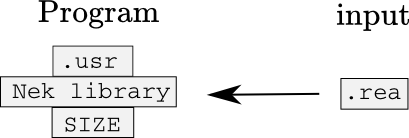
\includegraphics[width=0.5\textwidth]{Figures/filestructure2.png}
	\caption{Visualization of how the file structure in Nek5000 is built up.}
	\label{fig:files}
\end{figure}
%
To work with Nek5000 requires knowledge of some practicalities .
Nek5000 is recompiled for every case and the user specify all the case specific 
information in the three files \verb|{.rea,.usr,SIZE,}|. \verb|.usr| and \verb|SIZE| are 
compiled with the standard Nek5000 library using makenek which creates the executable file \verb|nek5000|,
they can be considered the surface and the core of the entire program. 
The \verb|.rea| file contains case-specific information read during the initialization of the 
compiled program. The user guide \cite{Nek} contains a tutorial which explains the necessary 
steps on how to get started with Nek5000. The next chapters will try to give some understanding on 
how the user is able to make the changes necessary for each case. \fref{fig:files} illustrates 
how the files work together. 
%
\subsection{SIZE}
Since Nek5000 is mostly based on Fortran77 all memory allocations are done statically and must be specified explicitly 
before runtime. Most of the variables used to determine the memory usage are stated in \verb|SIZE|.
The size of the working arrays necessary to perform the calculations are mostly defined by the upper limits of elements, 
processors, scalars and of course the polynomial degree
of the local Lagrange functions. These variables define the sizes of almost all 
the arrays used in the program so it is important to define these variables as accurately 
as possible to optimize memory usage. The \verb|SIZE| file can be considered as the necessary base 
for Nek5000.
%\begingroup
%\fontsize{12pt}{14pt}
%\begin{lstlisting}[escapechar=|,frame=none]
%parameter (ldim=3)                                   ! dimension
%parameter (lx1=6,ly1=lx1,lz1=lx1,lelt=600,lelv=lelt) ! GLL-points,elements/processor
%parameter (lxd=9,lyd=lxd,lzd=lxd)                    ! Order of De-aliasing
%\end{lstlisting}
%\endgroup
\subsection{.rea}

In \verb|.rea| all the problem specific parameters are given. While the content in \verb|SIZE| 
is an absolute necessity to even compile the program the \verb|.rea| file contains variables 
that are not used until the initialization of the case. The structure of the file is given in \tref{tab:reafile}.
Of the 103 variables specified in the beginning of the file there are roughly 50 of them that are used. 
Note that apart from the mesh information the \verb|.rea| file restricts itself to single variables and boolean flags 
while the \verb|.usr| needs to be applied for more advanced implementations. 
%
\begin{table}[h]
    \centering
    \begin{tabular}{c c l}
       Lines & Section Name & Specifications \\ \hline
       $103$ & PARAMETERS & All problem-specific variables \\ 
       $K$ & PASSIVE SCALAR DATA & Convective and diffusive constants for scalars\\ 
       $K$ & LOGICAL SWITCHES & Boolean variables defining the solution method \\ 
       $E$ & MESH DATA & All nodes and elements are specified here\\
       $E$ & CURVED SIDE DATA & All the curved sides are specified here\\
       $E$ & FLUID BC& BC type for all elements and their faces\\
       $E$ & THERMAL BC& Thermal BC type for all elements and their faces\\
       $K$ & PRESOLVE/RESTART & Filename(s) of an initialized solution \\
       $K$ & INITIAL CONDITIONS & possibilities to specify IC further \\
       $K$ & OUTPUT FIELD & information that will be written to file\\
    \end{tabular}
    \caption{An overview of the different sections in .rea. $E$ represents a predefined number depending on your problem
    which scales roughly as the number of elements, while $K\approx 1-25$ are user defined numbers.}
    \label{tab:reafile}
\end{table}
%
\subsection{.usr}
This file contains a series of standard routines open for modification by the user. In addition the user is free to specify 
new routines if needed. A description of these routines are given in the Nek5000 User manual~\cite{Nek}. A list of those 
frequently used for this thesis are described below, 
%routines used for this thesis are stated in \tref{tab:userfile}.
%
%\begin{table}
    %\centering
    %\begin{tabular}{c l}
        %Name & Description \\ \hline
        %\verb|userbc| & boundary conditions \\
        %\verb|uservp| & variable properties\\
        %\verb|userchk|& general purpose routine for checking errors etc.\\
        %\verb|usrdat2|& redifining mesh properties \\
        %\verb|usrdat3|& similar to usrdat2 \\
    %\end{tabular}
    %\caption{routines in .usr applied for this thesis.}
    %\label{tab:userfile}
%\end{table}
%
\begin{itemize}
    \item \verb|userbc| - Define the boundary conditions on the inflow-boundary. 
    \item \verb|uservp| - Define variable properties, impose the eddy viscosity when applying LES. 
    \item \verb|userchk| - Read inflow-data, and specify the output.
    \item \verb|usrdat2| - Project the geometry onto a deformed general surface. The details of how this routine is used will be 
    specified further in \cref{implementation}. 
    \item \verb|usrdat3| - Defines the interpolation algorithm that is applied to the inflow-data. 
\end{itemize}
%
In addition to these routines all user-defined functions are specified in this file. The LES implementation in Nek5000 is based
on several subroutines specified in addition to those stated above. A list of some of the variables and functions 
applied for the implementations in this thesis are stated in Appendix~\ref{AppendixB}.
The \verb|.usr| file can be considered as the surface of Nek5000, easily accessible for the user.

\section{The basics of the solver}
The most important building blocks in Nek5000 are the \verb|fluid| and \verb|heat| functions which solves the 
N-S and Passive scalar equations. The N-S solver works distinctly depending on the mathematical formulation
enabled whereas the PS equation, which does not depend on the pressure, is solved similarly for $P_NP_N$ and $P_NP_{N-2}$. 
For the sake of clarity, \fref{fig:files} shows how the algorithms are called from the main routine.
This is a simplified flow chart which does not include choices such as filters, preconditioners, LES-model, 
de-aliasing etc. but it explains how the two main algorithms are selected using the boolean variable \verb|ifsplit|. 
%
\begin{figure}[h]
	\centering
	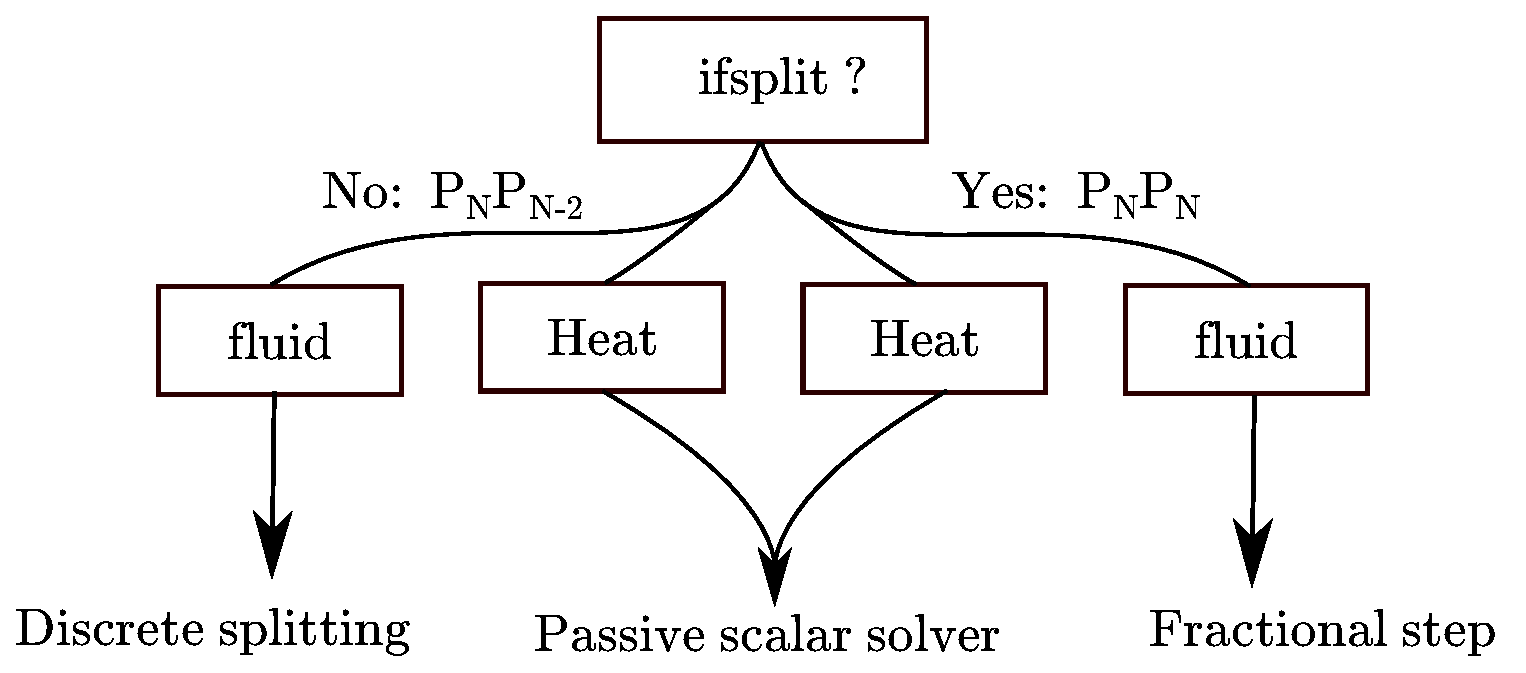
\includegraphics[width=0.8\textwidth]{Figures/Nek.pdf}
	\caption{Visualization of the steps in Nek5000.}
	\label{fig:files}
\end{figure}
%

The description of the routines corresponding to Pressure-correction and fractional step are found in 
\cref{prescorr} and~\ref{fracstep}. For further details regarding the 
implementation in Nek5000 it is referred to \cite{Fischer_hybridschwarz-multigrid}
and \cite{TomboulidesPnPn}. As mentioned before an important difference between these two implementations is the fact that the $P_NP_N$ 
implementation is based on an analytical splitting algorithm which introduces a non-vanishing error in the pressure along the boundaries of the 
domain while the $P_NP_{N-2}$ algorithm is a discrete splitting which does not explicitly force a wrong boundary condition.
It is however argumented in for instance~\cite{Guermond2006} that the discrete splitting also
introduces an erroneous boundary condition weakly.

%To best understand the work flow of Nek5000 the subroutine \verb|nek_advance| in \verb|drive1.f| should be examined.
%This routine includes all the steps in one iteration of the solver. The routine is adapted so that it is functional
%for a number of different problems and user defined settings. The most important boolean switches used in this routine are 
%described in the list below 
%
%\begin{itemize}
    %\item ifsplit - whether the $\mathbb{P}_N-\mathbb{P}_N$ or the $\mathbb{P}_N-\mathbb{P}_{N-2}$ is to be used.
    %\item iftrans - transient or steady flow.
    %\item ifheat - solving for heat.
    %\item ifnav - natural convection for the scalar fields (Boolean array)
    %\item param(103) - activation of filtering.
%\end{itemize}
%%
%further the routines of interests are \verb|fluid| and \verb|heat|, the solvers for N-S equations and passive scalars respectively.
%Both subroutines are found in \verb|drive2.f|. The understanding of these solvers are best achieved by studying equation  \eref{eq:NS} 
%and \eref{eq:PS}. For the settings chosen in this thesis a fractional step procedure as described in 
%\cref{fracstep} is applied.

%\colorbox{yellow}{what are fluidp() and heatp( )? solve for pertubated field and then project onto div-free space ? }

%\colorbox{yellow}{Talk about how the preconditioners work in Nek?}

%
%\section{Incompressible N-S solvers in Nek}
%Nek5000 offer several implementations depending on the mathematical formulation wanted by the user.
%The most standard, and the algorithm applied in this thesis is the fractional step procedure 
%described in detail in \cref{description}.


%A Convection-Diffusion problem can be stated as 
%\begin{align}
    %M\frac{du}{dt} = Au-Cu+Mf
    %\label{eq:conv-diff}
%\end{align}
%% 
%Where $M$ and $A$ is the mass, and stiffness matrix, $f$ is the loading function and $C$ is 
%the matrix corresponding to the convective term. The non-linearity is represented in the 
%convective term since $C$ is dependent of $u$.
%The time-derivative is discretized by a Backward difference (BDFk) scheme using solutions 
%from the $k$ previous steps to extrapolate the current value. In order to gain stability 
%an implicit scheme is chosen and the resulting eguation is given as 
%%
%OIFS ???
%---------- CHECK MAKEF IN NAVIER1.F ----------------- 
%\begin{align}
    %\sum_{j=0}^{k}\frac{b_j}{\Delta t}Mu^{n-j+1} = Au^{n+1}-Cu^{n+1}+Mf^{n+1}
    %\label{eq:conv-diff2}
%\end{align}
%% 
%By extrapolating the convective term from the $k$ previously calculated steps the equation 
%simplifies to 
%%
%\begin{align}
   %\frac{b_0}{\Delta t}Mu^{n+1} \sum_{j=1}^{k}\frac{b_j}{\Delta t}Mu^{n-j+1} 
   %= Au^{n+1}-\sum_{j=1}^{k}a_jCu^{n-j+1}+Mf^{n+1}
    %\label{eq:conv-diff3}
%\end{align}
%% 
%and finally by moving all the explicit terms to the rhs the equation left to solve is given as 
%%
%\begin{align}
   %(\frac{b_0}{\Delta t}M-A)u^{n+1} 
   %= -\sum_{j=1}^{k}(\frac{b_j}{\Delta t}M-a_jC)u^{n-j+1}+Mf^{n+1}
    %\label{eq:conv-diff4}
%\end{align}
%% 
%Notice from Section~\ref{theory} that this is equivalent to the matrix formulation of 
%the Helmholtz equation.



\section{Nek5000 for complex geometries}
For complex curved geometries such as bent cylinders, spheres, ellipsoids etc.
the user has to be able to express these surfaces analytically and write a routine
in \verb|usrdat2| that projects the points of interest onto the surface.
Even for a simple shape such as a sphere some implementation has to be done and it 
demands that the user has knowledge to Fortran77 and the structure of Nek5000.

The necessary implementation consists of two steps 
%
\begin{enumerate}
    \item determine the faces that belong to the deformed surface
    \item project the predefined GLL-points onto the deformed surface
\end{enumerate}
%
This can be done without too much work for shapes with a known analytical 
expression such as a cylinder or a sphere, but for some general CAD geometry 
it is no way to perform this projection routine. This is a vulnerable point 
for a SEM solver since the elements generated by the mesh are relatively coarse.
Many Finite volume based solvers do not support curved elements simply because the 
complex geometries are resolved with a sufficiently high resolution and it 
is of no interest to approximate them any better. However for a spectral element
solver it is necessary to address this problem since spectral convergence 
for the approximated solution in $\mathbb{P}_N$ is not achievable 
if the geometry is only represented in $\mathbb{P}_{1}$ or $\mathbb{P}_{2}$.

As a part of this thesis two advancements have been made regarding complex geometries. 
The first part is a fully automatic procedure which projects any edge onto a circle. This is a
convenient method when working with cylinder geometries and other similar shapes. The second part
is an attempt to include general boundary surfaces by creating a semi-automatic procedure allowing 
the user to represent any geometry with polynomials of the same order as applied for the basis functions.
The algorithms are presented in \cref{implementation}. 

% Chapter Template

\chapter{Implementation} % Main chapter title

\label{implementation} % Change X to a consecutive number; for referencing this chapter elsewhere, use \ref{ChapterX}

\lhead{Chapter 5. \emph{Implementation}} % Change X to a consecutive number; this is for the header on each page - perhaps a shortened title

%----------------------------------------------------------------------------------------
%	SECTION 1
%----------------------------------------------------------------------------------------

\colorbox{green}{Some introduction that motivates the work done in this thesis}

\colorbox{green}{henvis til NS, nevn eksplisitt de ligningene som brukes}

\colorbox{green}{Ta med et turbulensbilde, og bilde av plumen.}





\section{Case 1: Gas dispersion in a simplified urban area}
%The problem investigated in this work is gas dispersion of neutral gas in a velocity field through four cubic blocks.
%Similar simulations have been done in CDP and Fluent which are compared to data from a wind-tunnel experiment performed by ALAN.
The scenario investigated in this work is dispersion of a neutral gas in a rectangular tunnel
with four cubic blocks placed as obstacles. The blocks have sides $h = 0.109$m and represent a 
set of buildings forming a street canyon. The gas is released from a circular source on 
ground level and
is translated by the wind field through the canyon, see figure~\ref{fig:layout}.
In this figure $h$ have been used as the length scale. The dotted lines
indicates the positions where data is collected.
%
\begin{figure}[h]
	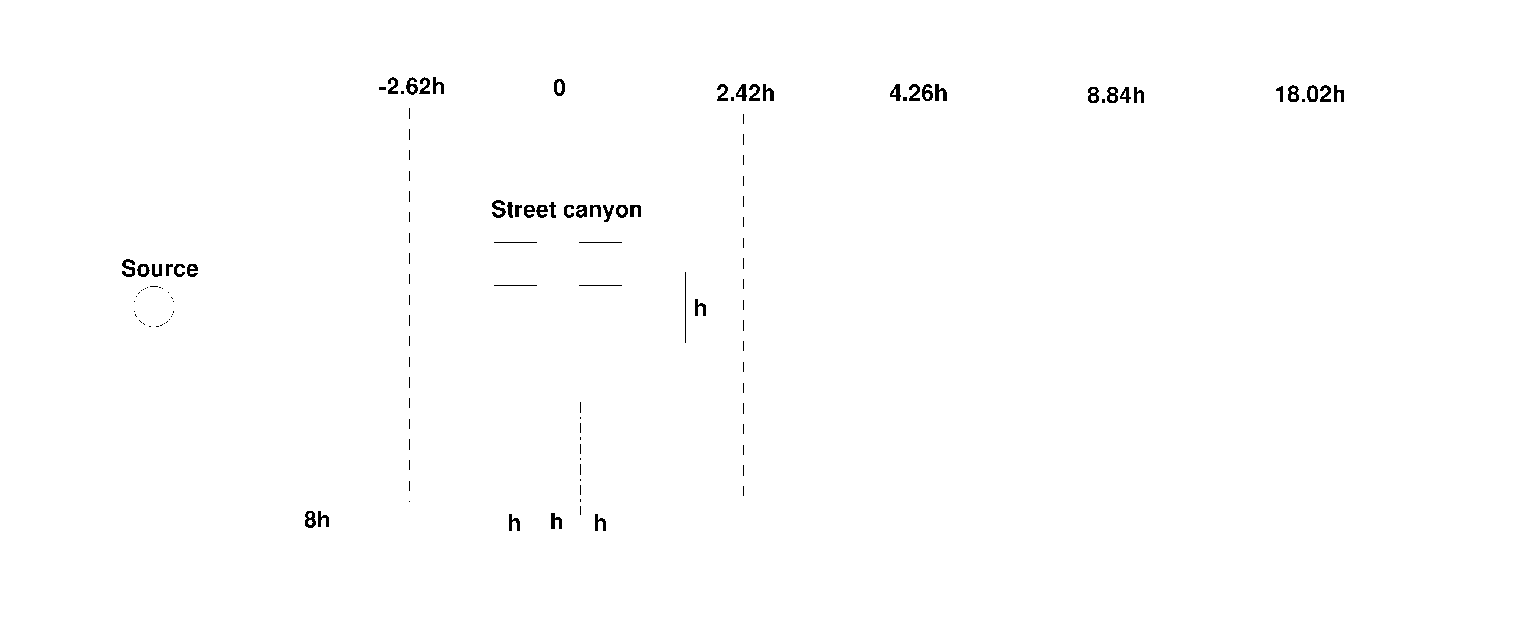
\includegraphics[width=1.1\textwidth]{Figures/layout.eps}
	\caption{Schematic overview of the domain from above. The data is collected along the dotted lines.}
	\label{fig:layout}
\end{figure}
%

Scaling the domain with the size of the boundary layer $H =1$m restricts it to
the box $0.0\leq x/H \leq 4.96,-1.75\leq y/H \leq 1.75, 0\leq z/H \leq 1.5$.
The four cubic boxes are centered around $(1.4315,0)$ with a distance $h$ between each box.
The source is placed with its center in $(0.396,0)$ and radius $r = 0.0515$.
The grid used for the computations consists of 4425 elements and with a polynomial degree of
12 the total number of nodes $N\approx 7,6$mill. 


The simulations are performed using Large Eddy Simulation (LES) 
with the dynamic Smagorinsky-Lilly subgrid-scale model. 
The release of gas will result in a plume that is advected with the wind field. The size and 
shape of the plume at the indicated positions in figure~\ref{fig:layout} are compared with 
experimental data and simulations performed in Fluent and CDP\@. 
The wind-field in the tunnel is created by an inflow condition that is defined from previous 
simulations in CDP~\cite{eriksson}.
For clarification some of the variables repeatedly mentioned throughout this thesis will be 
stated explicitly in table~\ref{tab:simplevariables}.
\begin{table}
    \centering
    \begin{tabular}{c c c c}
        Variable & value & unit & commentary \\ \hline
        $H$   & $1$ & m & length scale of the domain \\ 
        $h$   & $0.109$ & m & the sides of the cubic boxes\\ 
        $Q$   & $50$ & dm$^3$/min & gas release from source \\ 
        $U_{ref} $*& $\approx1.08$ & m/s & reference value of $U$ \\
    \end{tabular}
    \caption{Essential variables, *this value is calculated as a time average of the velocity in 
        x-direction at a point far away from the floor and walls and will therefore 
        vary a small amount from case to case. }
    \label{tab:simplevariables}
\end{table}

The inflow conditions had to be extrapolated onto the domain at each time step. The velocity field
on the inflow was generated in CDP, in order to create a boundary layer similar to the one found
in the wind-tunnel. The inflow velocity was written to file every 
$0.0013$s for a total of $28$ seconds. An interpolation algorithm had to be implemented in order
to adjust the inflow-data to each mesh. 
%
\begin{figure}[h]
    %\center
	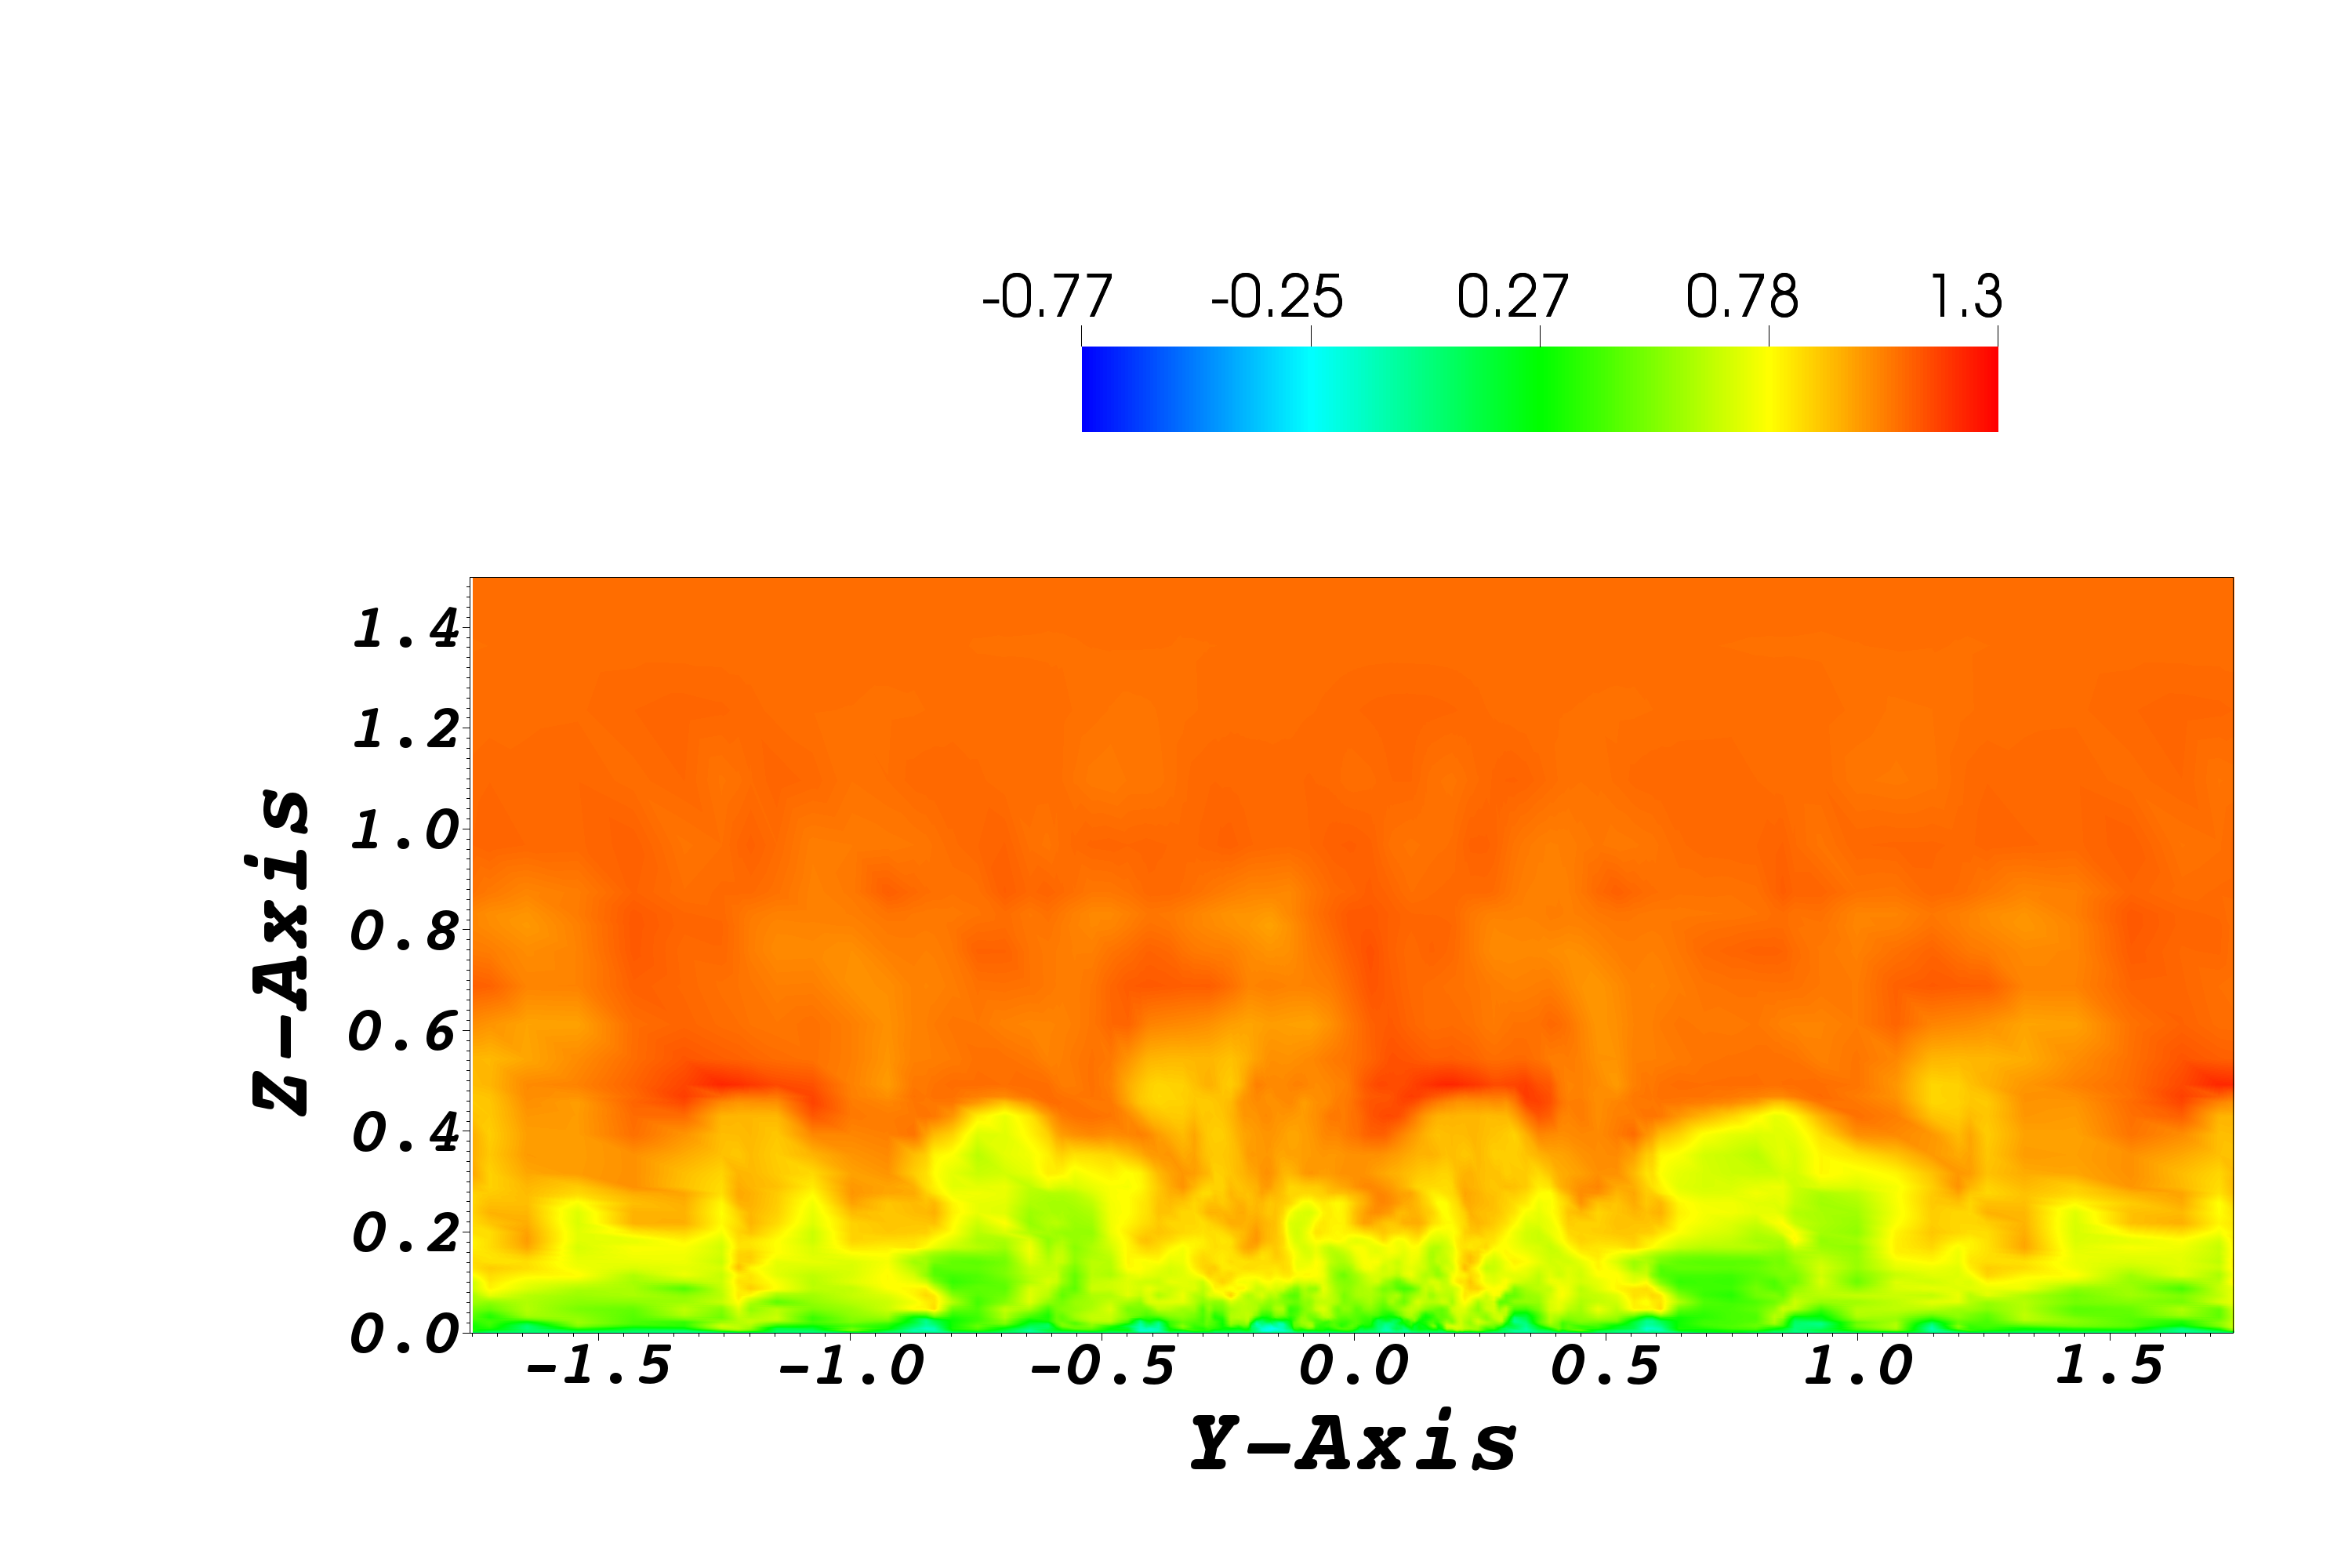
\includegraphics[width=0.5\textwidth]{Figures/inflow_field.png}
	\caption{X-velocity at inflow boundary, notice how the pattern copies itself}
	\label{fig:layout}
\end{figure}
%
\begin{figure}[h]
    %\center
	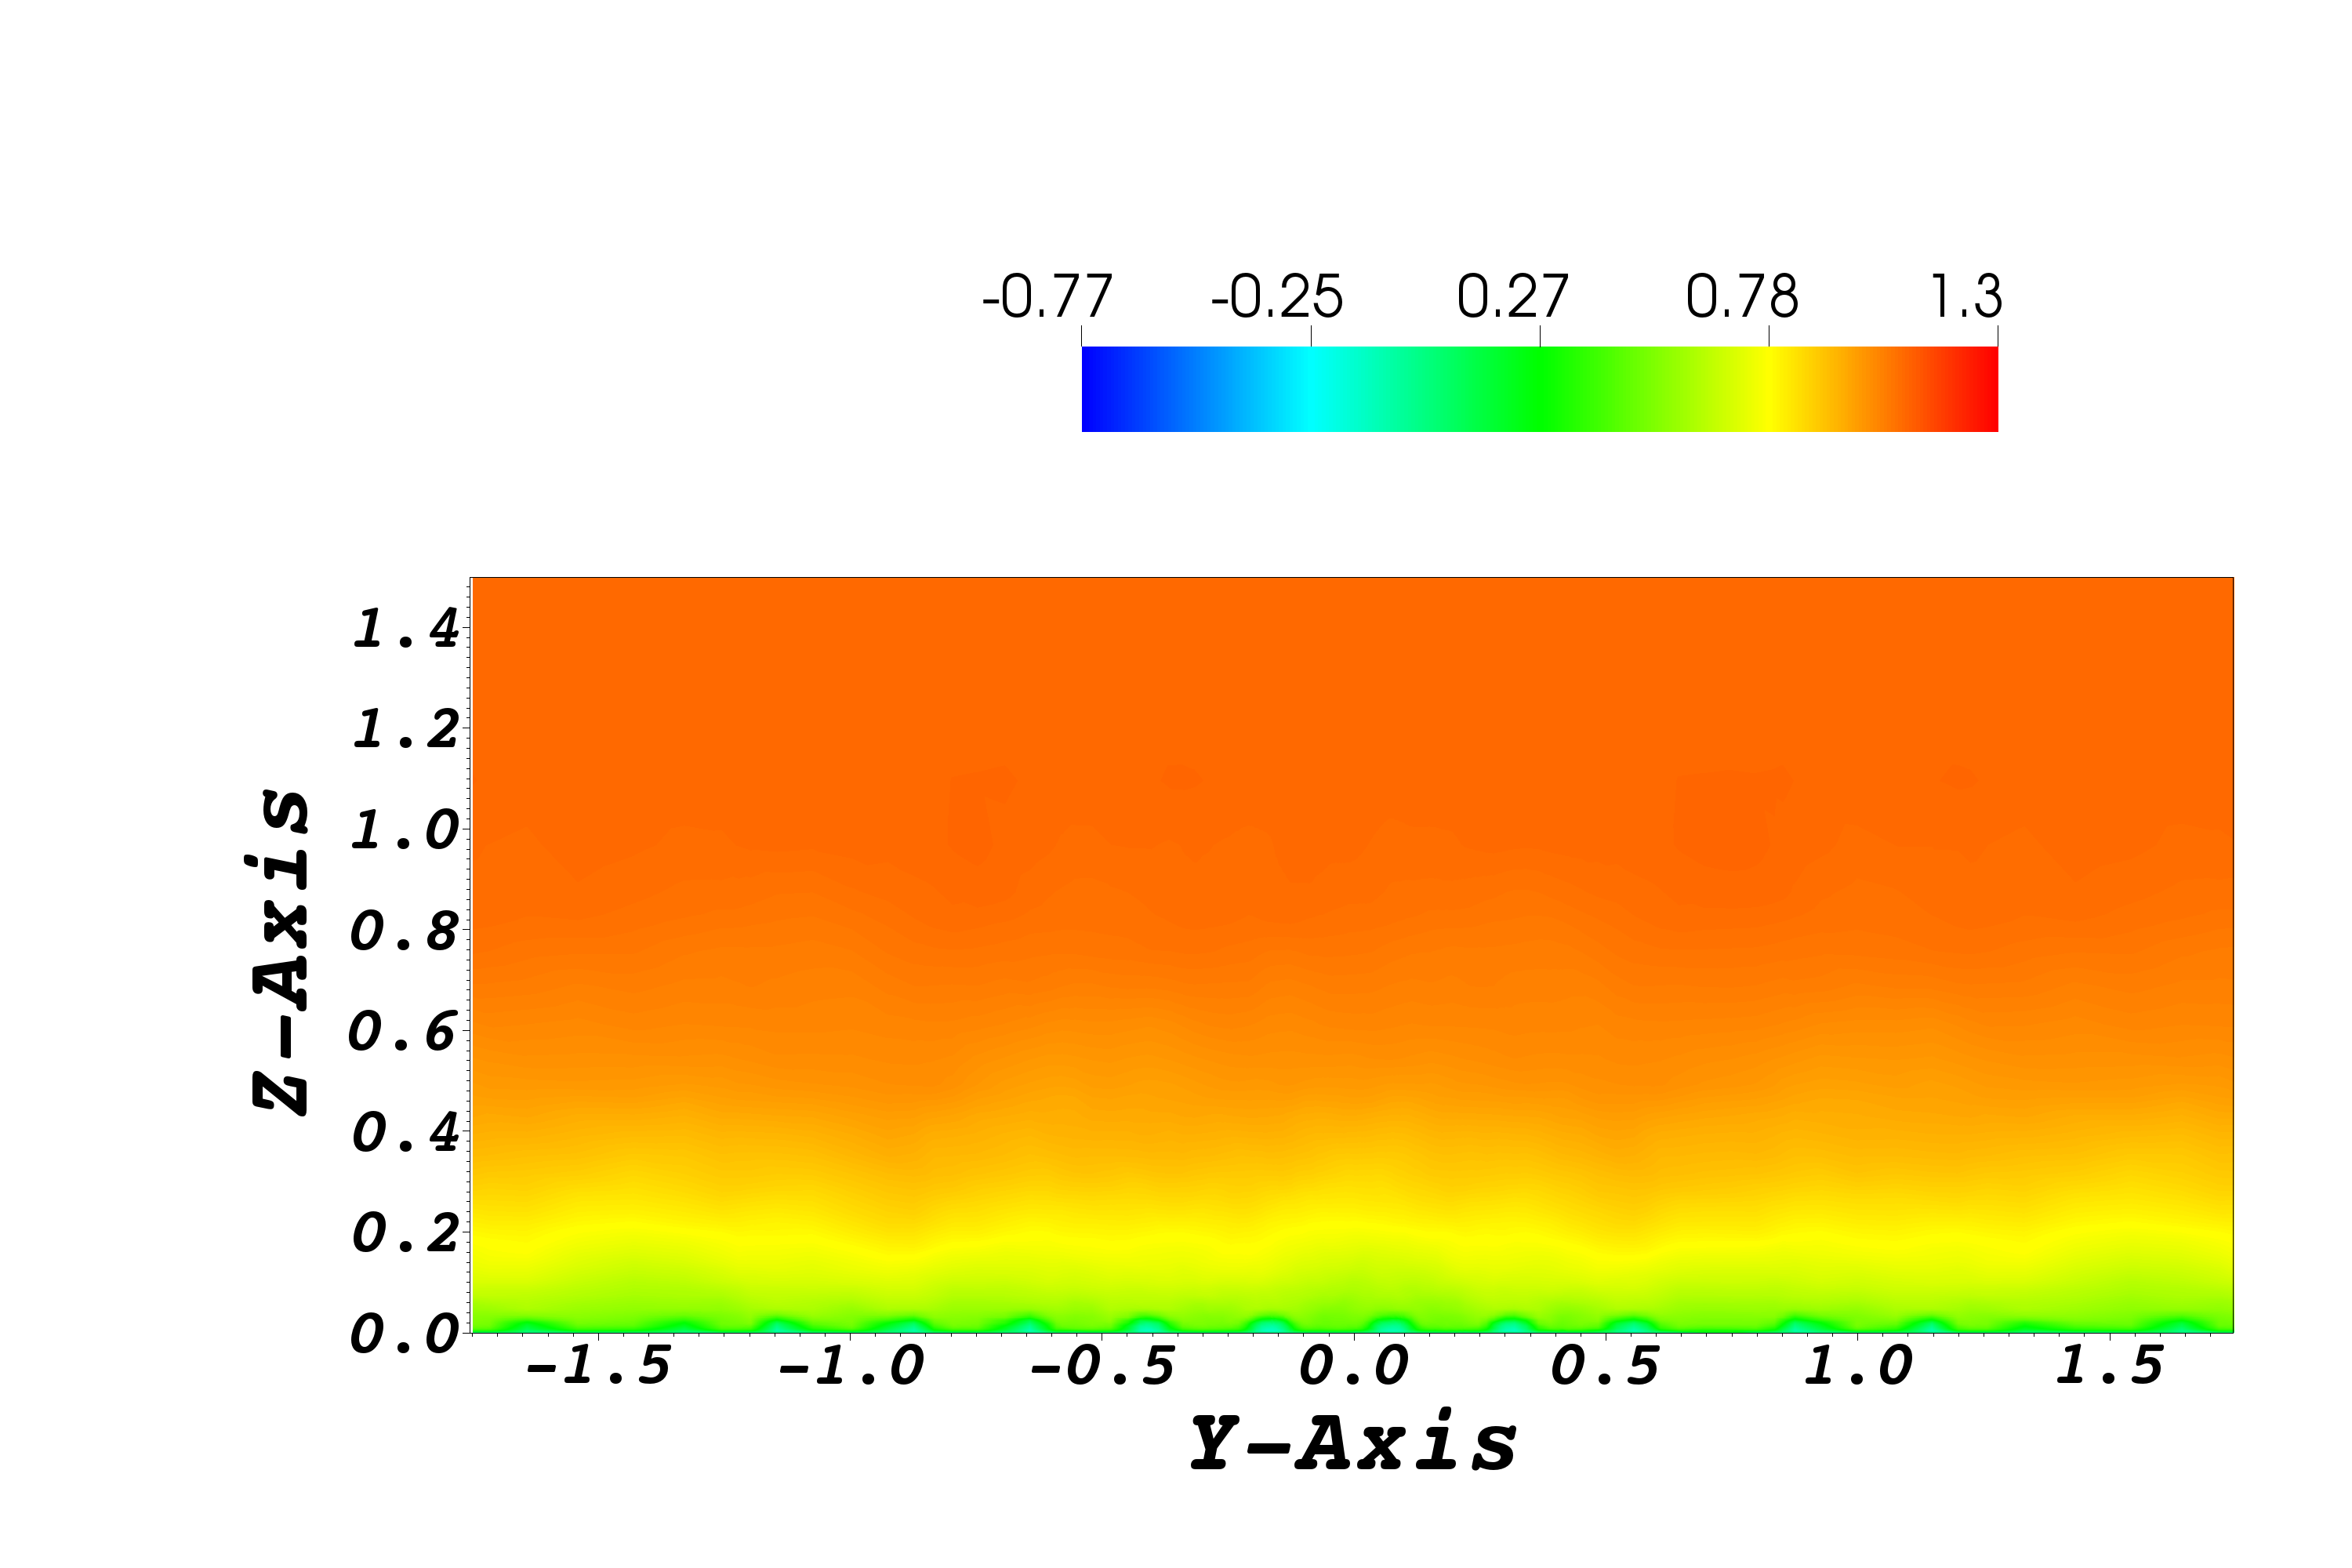
\includegraphics[width=0.5\textwidth]{Figures/inflow_field_avg.png}
	\caption{X-velocity at inflow boundary, notice how the pattern copies itself}
	\label{fig:layout}
\end{figure}
%
\section{Case 2: Drag and lift on a cylinder}
A standard benchmark case for flow solvers is presented in ~\cite{benchmark}.
The case is to calculate the drag and lift coefficients on a cylinder in a rectangular channel.
The setup for the domain and boundary conditions are given in figure~\ref{fig:cylinder}.
The constants applied in the description of the geometry and the coefficient scales are listed 
in table ~\ref{tab:case2consts}.
%
\begin{table}[h]
    \centering
    \begin{tabular}{c l l}
     Constant & Value & Property \\ \hline
    $H$ & $0.41\text{m}$ & Width and height for the channel \\
    $D$ & $0.1\text{m}$ & Diameter of the cylinder and length scale \\
    $U$ & $0.2\text{m/s}$ & Velocity scale \\
    $\nu$ &  $ 10^{-3}\text{m$^2$/s}$ & Kinematic viscosity of the fluid \\
    $Re$ & $20$ & Reynolds number \\ 
    \end{tabular}
    \caption{Constants for case 2}
    \label{tab:case2consts}
\end{table}
%
The flow is laminar with Reynolds number $Re=20$ so all the 
challenges arising when dealing with turbulent flow does not come to play in this case. 
The case will yield a steady state solution at which point the coefficients are calculated
and compared with the reference solutions.
\begin{figure}[h]
    \centering
    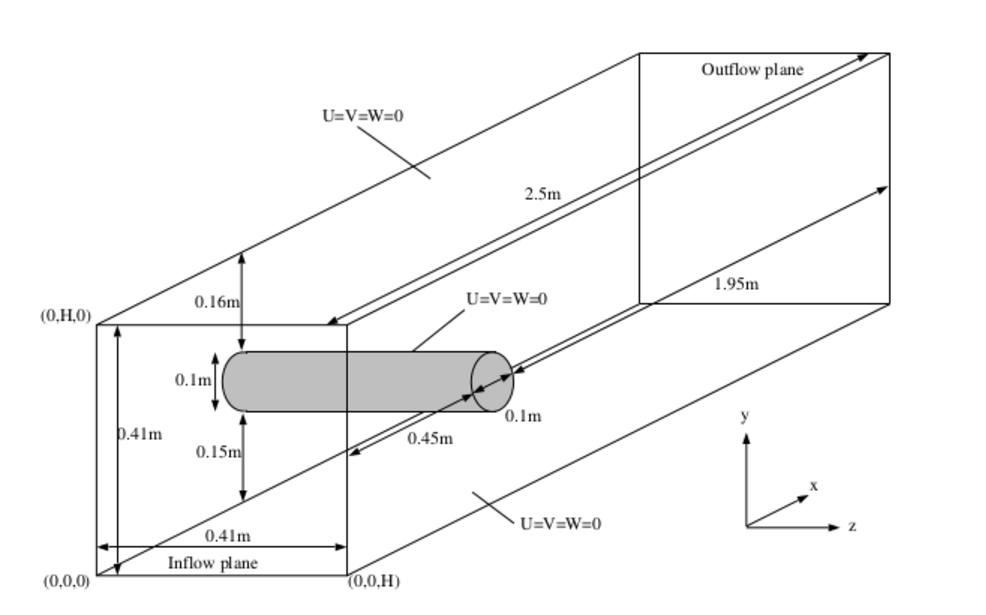
\includegraphics[width = 1.0\textwidth]{Figures/cylinder.pdf}
    \caption{Computational domain and boundary conditions.}
    \label{fig:cylinder}
\end{figure}
The spectral element method applied in Nek is known to be an accurate
solution method and is expected to 
provide a very good result in a test-case like this.
The drag and lift forces on an surface $S$ are given as 

\begin{align}
    F_D = \int_{S}(\rho \nu \frac{\partial v_t}{\partial n}n_y-pn_x)dS 
    \qquad , \qquad
    F_L = -\int_{S}(\rho \nu \frac{\partial v_t}{\partial n}n_x+pn_y)dS.
    \label{eq:dragnlift}
\end{align}


\colorbox{green}{Nevne hvordan integralet løses i Nek.}

\colorbox{green}{Dersom det var noen probmlemer med rammeverket, nevn det kort!}

\colorbox{green}{konsisten eq. bruk! }

The coefficients corresponding to these forces known as the drag and lift coefficients 
are given by the formulas 
\begin{align}
    c_D = \frac{2F_D}{\rho U^2 D H}
    \qquad , \qquad
    c_L = \frac{2F_L}{\rho U^2 D H}.
    \label{eq:dragnliftcoeffs}
\end{align}
Nek provides functions for calculating lift and drag on any user-specified object.
The function is called \verb|drag_calc(scale)|, with the input parameter 
defined by the user, for this case \verb|scale|$=2/(\rho U^2DH)$.  
Apart from this the function \verb|set_obj()| has to be modified in order to create an object 
which consists of all the faces on the cylinder.
Let $x,y$ be points in the computational domain, $x_c,y_c$ be the coordinates to the 
center line in the cylinder and $0<tol\ll1$ be some user defined tolerance. The faces that belong to the cylinder can then be found by 
looping over all elements and their faces evaluating $\epsilon = \sqrt{(x-x_c)^2+(y-y_c)}$.
If $\epsilon < tol$ for an entire face then this face is known to 
belong to the cylinder and is added to the object. Nek also allows the user to specify multiple objects 
assigning the faces of interest to object 1, object 2 etc. The geometry and mesh 
for this case was generated in ICEM, and the total number of elements are 2070. 
For the final calculation polynomial degree $P = 11$ was applied leading to a 
total of $N = 2755170$.

%
\begin{figure}[h]
    \centering
    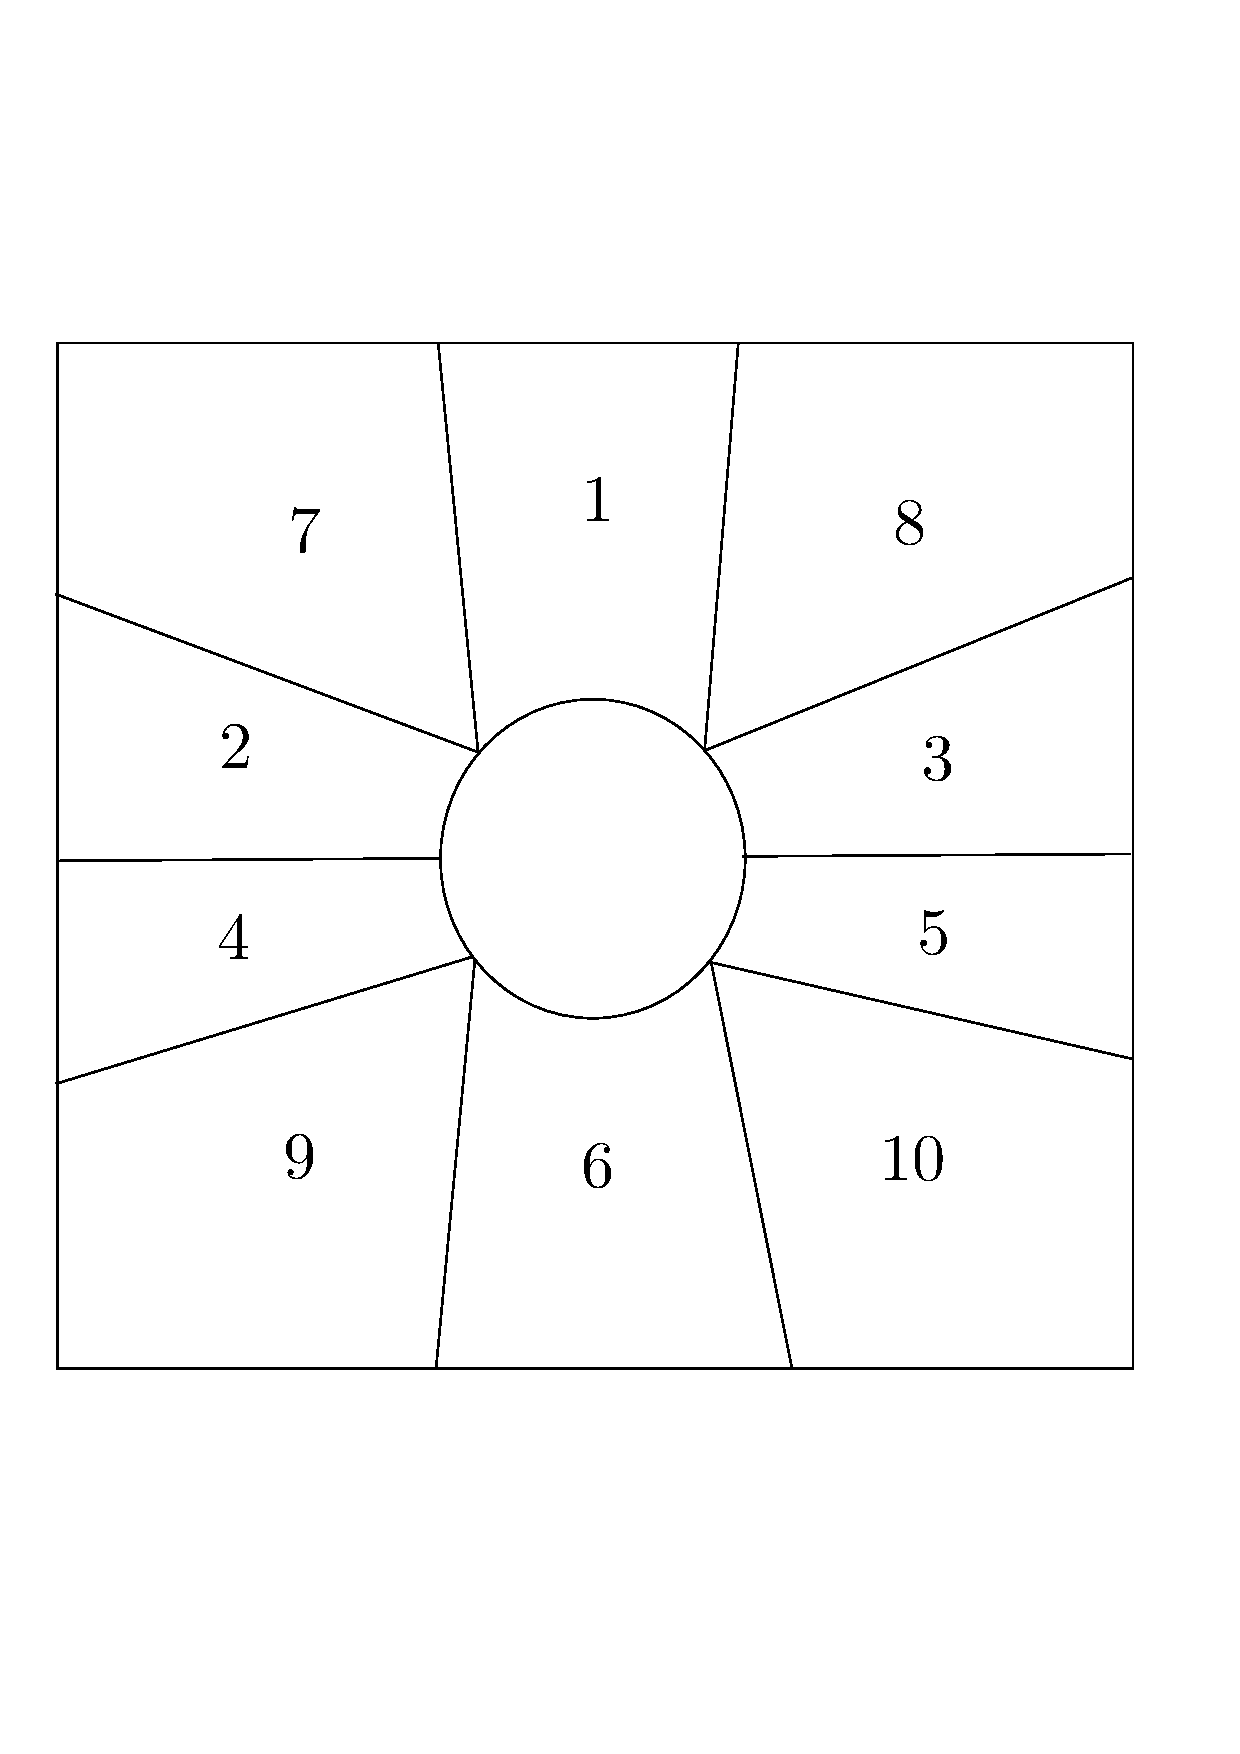
\includegraphics[width = 0.4\textwidth]{Figures/cyl_elem.pdf}
    \caption{Initial mesh around cylinder.}
    \label{fig:cyl_elem}
\end{figure}
%
Initially this case was solved using a second degree polynomial to describe the circle segments
corresponding to each element. The mesh around the cylinder is illustrated in figure~\ref{fig:cyl_elem}.
Note that these elements was split in three, in order to obtain 
a finer mesh in the region of interest. Of the elements numbered in~\ref{fig:cyl_elem}
only the first six contains edges on the cylinder.Hence the second order polynomials 
describing the curved edges describe approximately $\Theta = 360^{\circ}/(6\cdot 3) = 20^{\circ}$
of the complete circle. There is no computational reason 
for not incorporating an order $n=P$ approximation of the circle segments eliminating 
this approximation error. An algorithm was therefore implemented as an extension to the
currently available features regarding curvature on edges.
The full description of the algorithm is presented in 
chapter~\ref{xyzarc}. The importance of the error resulting from the second degree approximation
of the circle segments are presented in chapter~\ref{results}.
%
%
%
\section{Advances in the mesh-generation routine} \label{xyzarc}
The routine \verb|xyzarc()|:

The Gordon Hall algorithm was already implemented as a function in Nek, with the GLL-points,polynomial degree and some initial 
coordinates to the element. The algorithm creates a distribution of the internal GLL-points in each element. 
If the element consists of linear edges the only necessary input are the vertices, but by specifying the points on edges and faces
the algorithm creates a logical distribution of the internal GLL-points to a deformed element. 

The curved edge is specified in the .rea file and the routine \verb|genxyz()| processes the input of each edge. 
By specifying the radius and the circle center \verb|genxyz()| calls the routine \verb|xyzarc()| which performs the following algorithm;

$a,b$ will be the two end nodes of the edge 
$c$ will be the mid node, 
$s$ will be the arc length, 
$\theta$ will be the full angle of the circle sector,
$cc$ is the center coordinates, 
$g$ will be the vector containing the GLL-points in $[-1,1]$ 
and $r$ will be the radius.

\begingroup
%\fontsize{12pt}{14pt}
\begin{lstlisting}[escapechar=|,frame=none]
 l = a-b                       ! vector between the corner nodes
 c = (a+b)/2                   ! midpoint location
 h = c-cc                      ! height of the framed triangle
 |$\theta$| = arctan(abs(l)/2*abs(h))    ! half the angle of the circle sector
 s = r*|$\theta$|                       ! arc length
 g = g*|$\theta$|                      ! angles to the GLL-points on the circle-sector
 !---------- Finding the intersecting points ----------!
 !---- x on the line l, and extend x-cc to the arc ----!
 do k=1,lx1          ! for the number of nodes in one direction
    |$\alpha$| = h*tan(g[k])           ! offset from the midpoint on l
    x = c-|$\alpha$|*l/abs(l)           ! actual coordinate on l
    m = x-cc                   ! hypotenuse of the imposed triangle
    edge(k) = cc+r*m/abs(m)    ! final coordinate on the arc
 enddo
\end{lstlisting}
\endgroup
These lines creates the wanted edge curved as a circle sector corresponding to the radius and circle center given.
The remaining operation is to call the Gordon Hall algorithm and create the internal GLL-points defined by the edges 
provided. The figure~\ref{fig:curvature} illustrates the geometry on which the algorithm is performed.
Notice that the algorithm assumes that the center $c$ is somewhere on the plane defined as all the 
points with equal distance to both $a$ and $b$.


\begin{figure}[h]
    \centering
    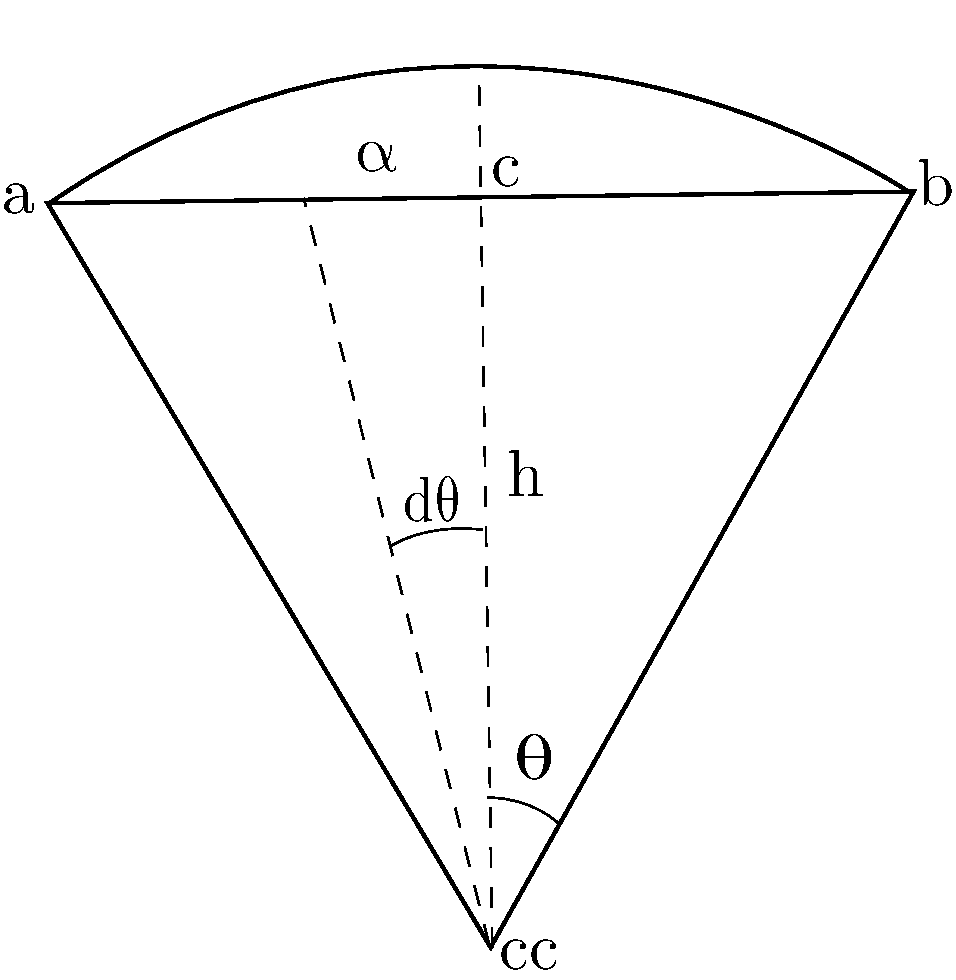
\includegraphics[width = 0.5\textwidth]{Figures/curvature.pdf}
    \caption{A sketch of the curved edge and the variables necessary to calculate the projection}
    \label{fig:curvature}
\end{figure}


\begin{itemize}
	\item initial script
	\item changes and modifications
	\item performance testing
	\item pitfalls
\end{itemize}


\section{Additional projection algorithm}\label{surfpro}
The routine \verb|xyzarc()| enables the user to represent circular edges with the same order as
the Lagrange polynomials of each element. For more complex geometry such as actual 
terrain and other surfaces without any analytic expression the large element sizes 
makes the geometrical representation difficult. There is however no reason why the 
GLL-points on a face can be projected onto a non-analytical surface. Although there
are no support for automatically reading additional information for distributing the 
GLL-points exactly on a given surface a routine was made which demands a minimum of 
manual work. The method can be summed up in these simple steps
\begin{enumerate}
    \item Create initial Mesh and convert to .rea applying nmshconvert.
        \item Create refined surface mesh on the non-regular surface.
        \item Enable projection by setting param(33) = 1.
        \item Choose number of interpolation points by modifying param(34)= (1,2,3)
\end{enumerate}

In addition to the standard Nek library the file surfpro.f needs to be added to 
the /trunk/nek/ folder along with all the other scripts applied by Nek.

The algorithm relies on two external files generated by the modified nmshconvert script.
\verb|surf.i| contains all the coordinated to the points on the refined surface. 
\verb|bdry.i| contains the element, and face number to all the faces to be projected onto the surface.
When generated they automatically alter the local \verb|SIZE| file to contain some key variables 
applied in the algorithm in surfpro.f.
The algorithm is best explained through a simple box with a non-regular floor. 
As an initial test-problem the hill of Ekeberg was applied. 
Before describing the algorithm let $E_{tot} = n_xn_yn_z$  be the total number of elements, 
$N$ is the polynomial degree and let us for simplicity assume that $n_x=n_y=n_z$ such that 
$E= E_{tot}^{2/3}$ is the number of elements containing a face on the non-regular surface.
The number of points on the refined surface $N_s$ should be somewhat larger than $EN^2$ in 
order to describe the surface for all the GLL-points that belong to the boundary. 
The pseudo code for the algorithm is listed below.
%
\begingroup
\fontsize{12pt}{14pt}
\begin{lstlisting}[escapechar=|,frame=none]
do e,f in bdry.i
  wrk = create_working_surface(e,f)
  do i in GLL-nodes
    interp = init_interpolation_array() 
    do j in wrk
       update_int_array(interp,wrk(j))
    enddo
    set_new_point(interp,wrk,i,e,f)
  enddo
  fix_GLL()
enddo
fix_geom()
\end{lstlisting}
\endgroup
% 
In order to understand the algorithm a short description of the auxiliary functions is 
given in the list below
\begin{itemize}
    \item create\_working\_surface(e,f) -- Loops through all the nodes in surf.i and adds the 
        surface-coordinates within a certain radius to the center GLL-node to the array wrk.
        This saves time in the search for interpolation points for each GLL-node.
    \item init\_interpolation\_array() -- initializing the array containing the closest 
        points on the surface for the current GLL-node. 
    \item update\_int\_array(interp,wrk(j)) -- compares the current surface point to the 
        already existing interpolation points and adds it to the list if it is found to 
        be closer to the initial GLL-node.
    \item set\_new\_point(interp,wrk,i,e,f) -- updating the new GLL-point determined by the 
        surface points in interp.
    \item fix\_GLL() -- There is a risk after distributing the GLL-points on the surface that
        some of the internal GLL-points falls outside the element. fix\_GLL() distributes 
        all internal GLL-points correctly between the newly projected face and the opposite.
    \item fix\_geom() -- An already existing Nek routine which redistributes the GLL-points to 
        assure that the distance between them on the new surface are correct.
\end{itemize}

Although this routine is only called once, and therefore will not contribute significantly 
to the total runtime of the program it is desirable to have a fast algorithm. Another analysis
important to be made is the amount of extra storage space needed for this algorithm.
By analysing the pseudo code the time of the algorithm should be of order $O(EN^2(E+N^2))$
and the amount of additional storage space will be of order $O(EN^2+E+N^2)=O(EN^2)$.

The routine attempts to be as automatic as possible and the only implementation necessary is 
a call from \verb|usrdat2| with 3 input variables.

Now an illustrative example of how this method is applied by the user. Say you have a project
called ''myFlow'', and the mesh and surface mesh created in ICEM are named mesh\_myFlow and 
surfmesh\_myFlow. The following commands are then executed

%
%\begin{lstlisting}[style=FormattedNumber, basicstyle = \ttfamily,frame= none]
%>> ~/path/to/meshconvert/scrpt/nmshconvert --mesh mesh_myFlow 
%--reafile init.rea --outfile myFlow.rea
%--tol 1e3 --temperature True --curvetype A

%>> ~/path/to/meshconvert/scrpt/nmshconvert --mesh surfmesh_myFlow --mesh_format surface
%\end{lstlisting}
% 
\begingroup
\fontsize{12pt}{14pt}
\begin{lstlisting}[escapechar=|,frame=none]
>> /nmshconvert --mesh mesh_myFlow 
    --reafile init.rea --outfile myFlow.rea
    --tol 1e3 --temperature True --curvetype A

>> ./nmshconvert --mesh surfmesh_myFlow 
    --mesh_format surface

\end{lstlisting}
\endgroup
% 
% 
%\begin{lstlisting}[style=FormattedNumber, frame=none]
    %int* p;
    %int a[4];
    %p = a;
%\end{lstlisting}
\subsection{Application on the hill of Ekeberg}
As an initial test of the algorithm a mesh was created based on the hill of Ekeberg.
The surface was loaded as a \verb|.tin| file in ICEM and a simple box was created with 
the described terrain as floor. A simple sketch of the domain with the initial mesh in given in 
figure~\ref{fig:ekeberg}. This geometry was chosen because it resembles a typical problem with 
spectral elements. Since the initial element-mesh is relatively coarse it does not capture all 
the details in the geometry and the GLL-nodes distributed on the faces corresponding to the 
unstructured surface will be misplaced. It is however no theoretical problem to reconstruct the 
surface with with a polynomial of order $P$. With the routine described in chapter~\ref{surfpro}
The surface was approximated accurately by higher order polynomials.
%
\begin{figure}[t]
    \centering
	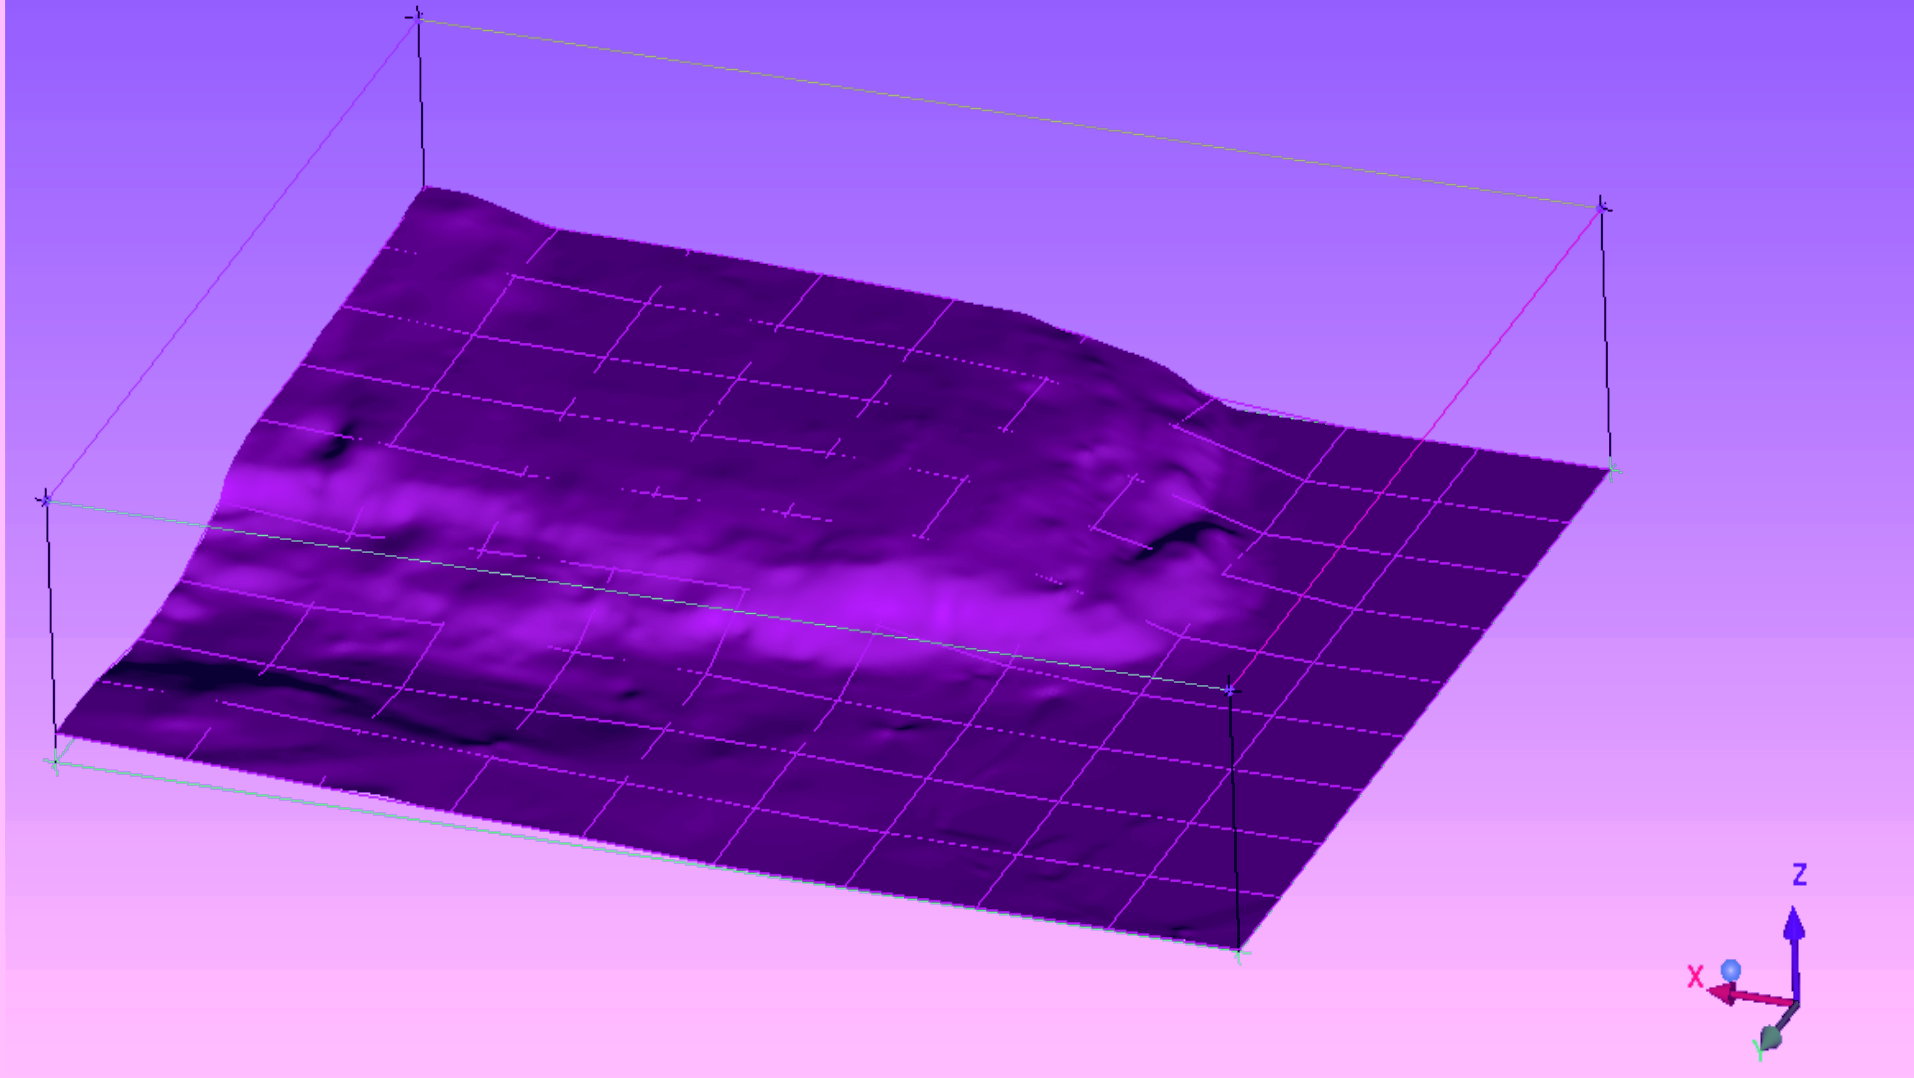
\includegraphics[width=0.7\textwidth]{Figures/mesh_ekebergaasen2.png}
    \caption{The initial mesh of the hill}
	\label{fig:ekeberg}
\end{figure}
%
The algorithm restricts itself to relatively smooth surfaces.
\section{Spatial averaging routine}
A dynamic Smagorinsky model has previously been implemented in Nek5000 for flow in a channel. 
The method as described in chapter~\ref{description} depends on an averaging routine to calculate
the dynamic Smagorinsky constant. The implementation in Nek applies an average routine in the plane,
assuming that the Smagorinsky constant is the same for all points with equal distance to the walls 
of the channel. This is a rather specific averaging routine only applicable to channel flows.

When applying dynamical Smagorinsky to Case 1 a new spatial mean routine had to be applied. 
It was first attempted to average only in time, but this proved not to be sufficient. It was
therefore implemented a simple routine for taking the average within each element, let 
$c_{num}^e,c_{den}^e$ denote the numerator and the denominator in equation~\ref{eq:dynsmag}.
The means are then calculated as 
\begin{align}
    c_{num}^e = \frac{1}{V}\int_{\Omega_e}c_{num}^e d\: \Omega 
    = \frac{1}{V}\sum_{i = 1}^{N^3}\rho_{i,e}c_{num,i}^{e}.
    \label{eq:averageroutine}
\end{align}
And similarly for $c_{den}^e$.
The coefficients $\rho_{i,e}$ are found in the array \verb|BM1(lx1,ly1,lz1)| in the file 
\verb|MASS|.
 
% Chapter 6

\chapter{Case studies and results} % Main chapter title

\label{results} % For referencing the chapter elsewhere, use \ref{Chapter1} 

\lhead{Chapter 6. \emph{Results and Discussion}} % This is for the header on each page - perhaps a shortened title

%----------------------------------------------------------------------------------------

This chapter will present the cases investigated and the results achieved.
The main tools in addition to Nek5000 needed to perform the simulations presented in this 
chapter are \textit{ANSYS ICEM} and \textit{python}. For post-processing \textit{Visit} and
\textit{Matlab} were used.
%
\section{Case 1: Gas dispersion in a simplified urban area}
%The problem investigated in this work is gas dispersion of neutral gas in a velocity field through four cubic blocks.
%Similar simulations have been done in CDP and Fluent which are compared to data from a wind-tunnel experiment performed by ALAN.
The scenario investigated in this work is dispersion of a neutral gas in a rectangular tunnel
with four cubic blocks placed as obstacles. The blocks have sides $h = 0.109$m and represent a 
set of buildings forming a street canyon. The gas is released from a circular source on 
ground level and
is translated by the wind field through the canyon, see \fref{fig:layout}.
In this figure $h$ have been used as the length scale. The dotted lines
indicate the positions where data is collected.
%
\begin{figure}[h]
	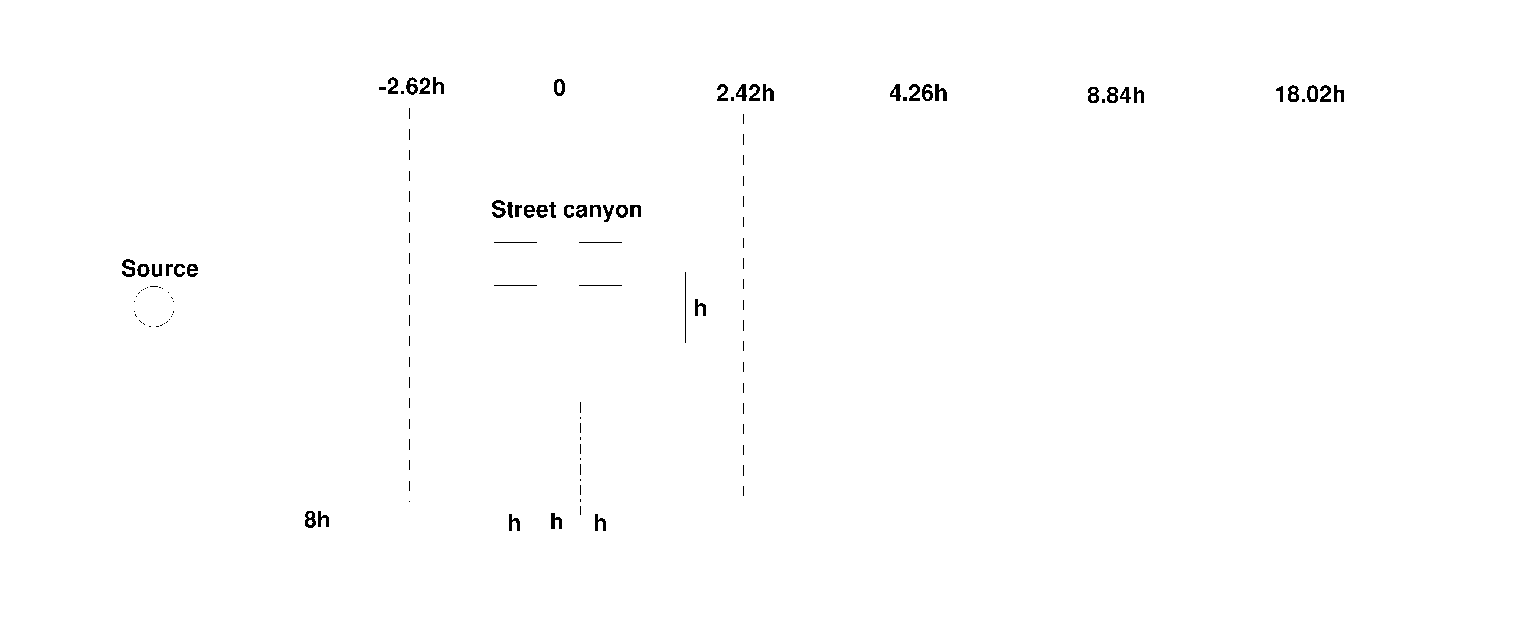
\includegraphics[width=1.1\textwidth]{Figures/layout.eps}
	\caption{Schematic overview of the domain from above. The data is collected along the dotted lines.}
	\label{fig:layout}
\end{figure}
%

Scaling the domain with the size of the boundary layer $H =1$m restricts it to
the box $0.0\leq x/H \leq 4.96,-1.75\leq y/H \leq 1.75, 0\leq z/H \leq 1.5$.
The four cubic boxes are centered around $(1.4315,0)$ with a distance $h$ between each box.
The source is placed with its center in $(0.396,0)$ and radius $r = 0.0515$.
The grid used for the computations consists of 14747 elements and with a polynomial degree of
7 the total number of nodes $N\approx 5,2$mill. 


The simulations are performed using Large Eddy Simulation (LES) 
with the dynamic Smagorinsky-Lilly subgrid-scale model and by applying the polynomial filtering
routine that is available in Nek5000. 
The release of gas will result in a plume that is advected with the wind field,
see \fref{fig:plume}. The concentration of the released gas at the 
indicated positions in \fref{fig:layout} are compared with 
experimental data and simulations performed in CDP~\cite{CDP}. 
For clarification some of the variables repeatedly mentioned throughout this thesis will be 
stated explicitly in \tref{tab:simplevariables}.
\begin{table}
    \centering
    \begin{tabular}{c c c c}
        Variable & value & unit & commentary \\ \hline
        $H$   & $1$ & m & length scale of the domain \\ 
        $h$   & $0.109$ & m & the sides of the cubic boxes\\ 
        $Q$   & $50$ & dm$^3$/min & gas release from source \\ 
        $U_{ref} $& $\approx1.08$ & m/s & reference value of $U$ \\
    \end{tabular}
    \caption{Essential variables, $U_{ref}$ is calculated as a time average of the velocity in 
        x-direction at a point far away from the floor and walls and will therefore 
        vary by a small amount from case to case. }
    \label{tab:simplevariables}
\end{table}

The inflow conditions had to be extrapolated onto the domain at each time step. To mimic the situation in the wind-tunnel the velocity field
on the inflow was generated in a different simulation performed in CDP. The inflow velocity was written to file every 
$0.0013$s for a total of $28$s and had to be interpolated onto the domain for the simulations in Nek5000 since the grid was not identical.
The right plot in \fref{fig:inflow} is an instantaneous picture of the inflow velocity in x-direction, 
notice how the pattern repeats itself along the y-axis. This is because the inflow data was generated in a smaller channel, approximately $1/3$ of the 
width of the computational domain used for the data sampling. An interpolation algorithm implemented at FFI was applied to adjust 
the inflow-data to the computational mesh, this was done directly in \verb|.usr|. 
%
\begin{figure}
\centering
  \centerline{
\begin{minipage}{.6\textwidth}
  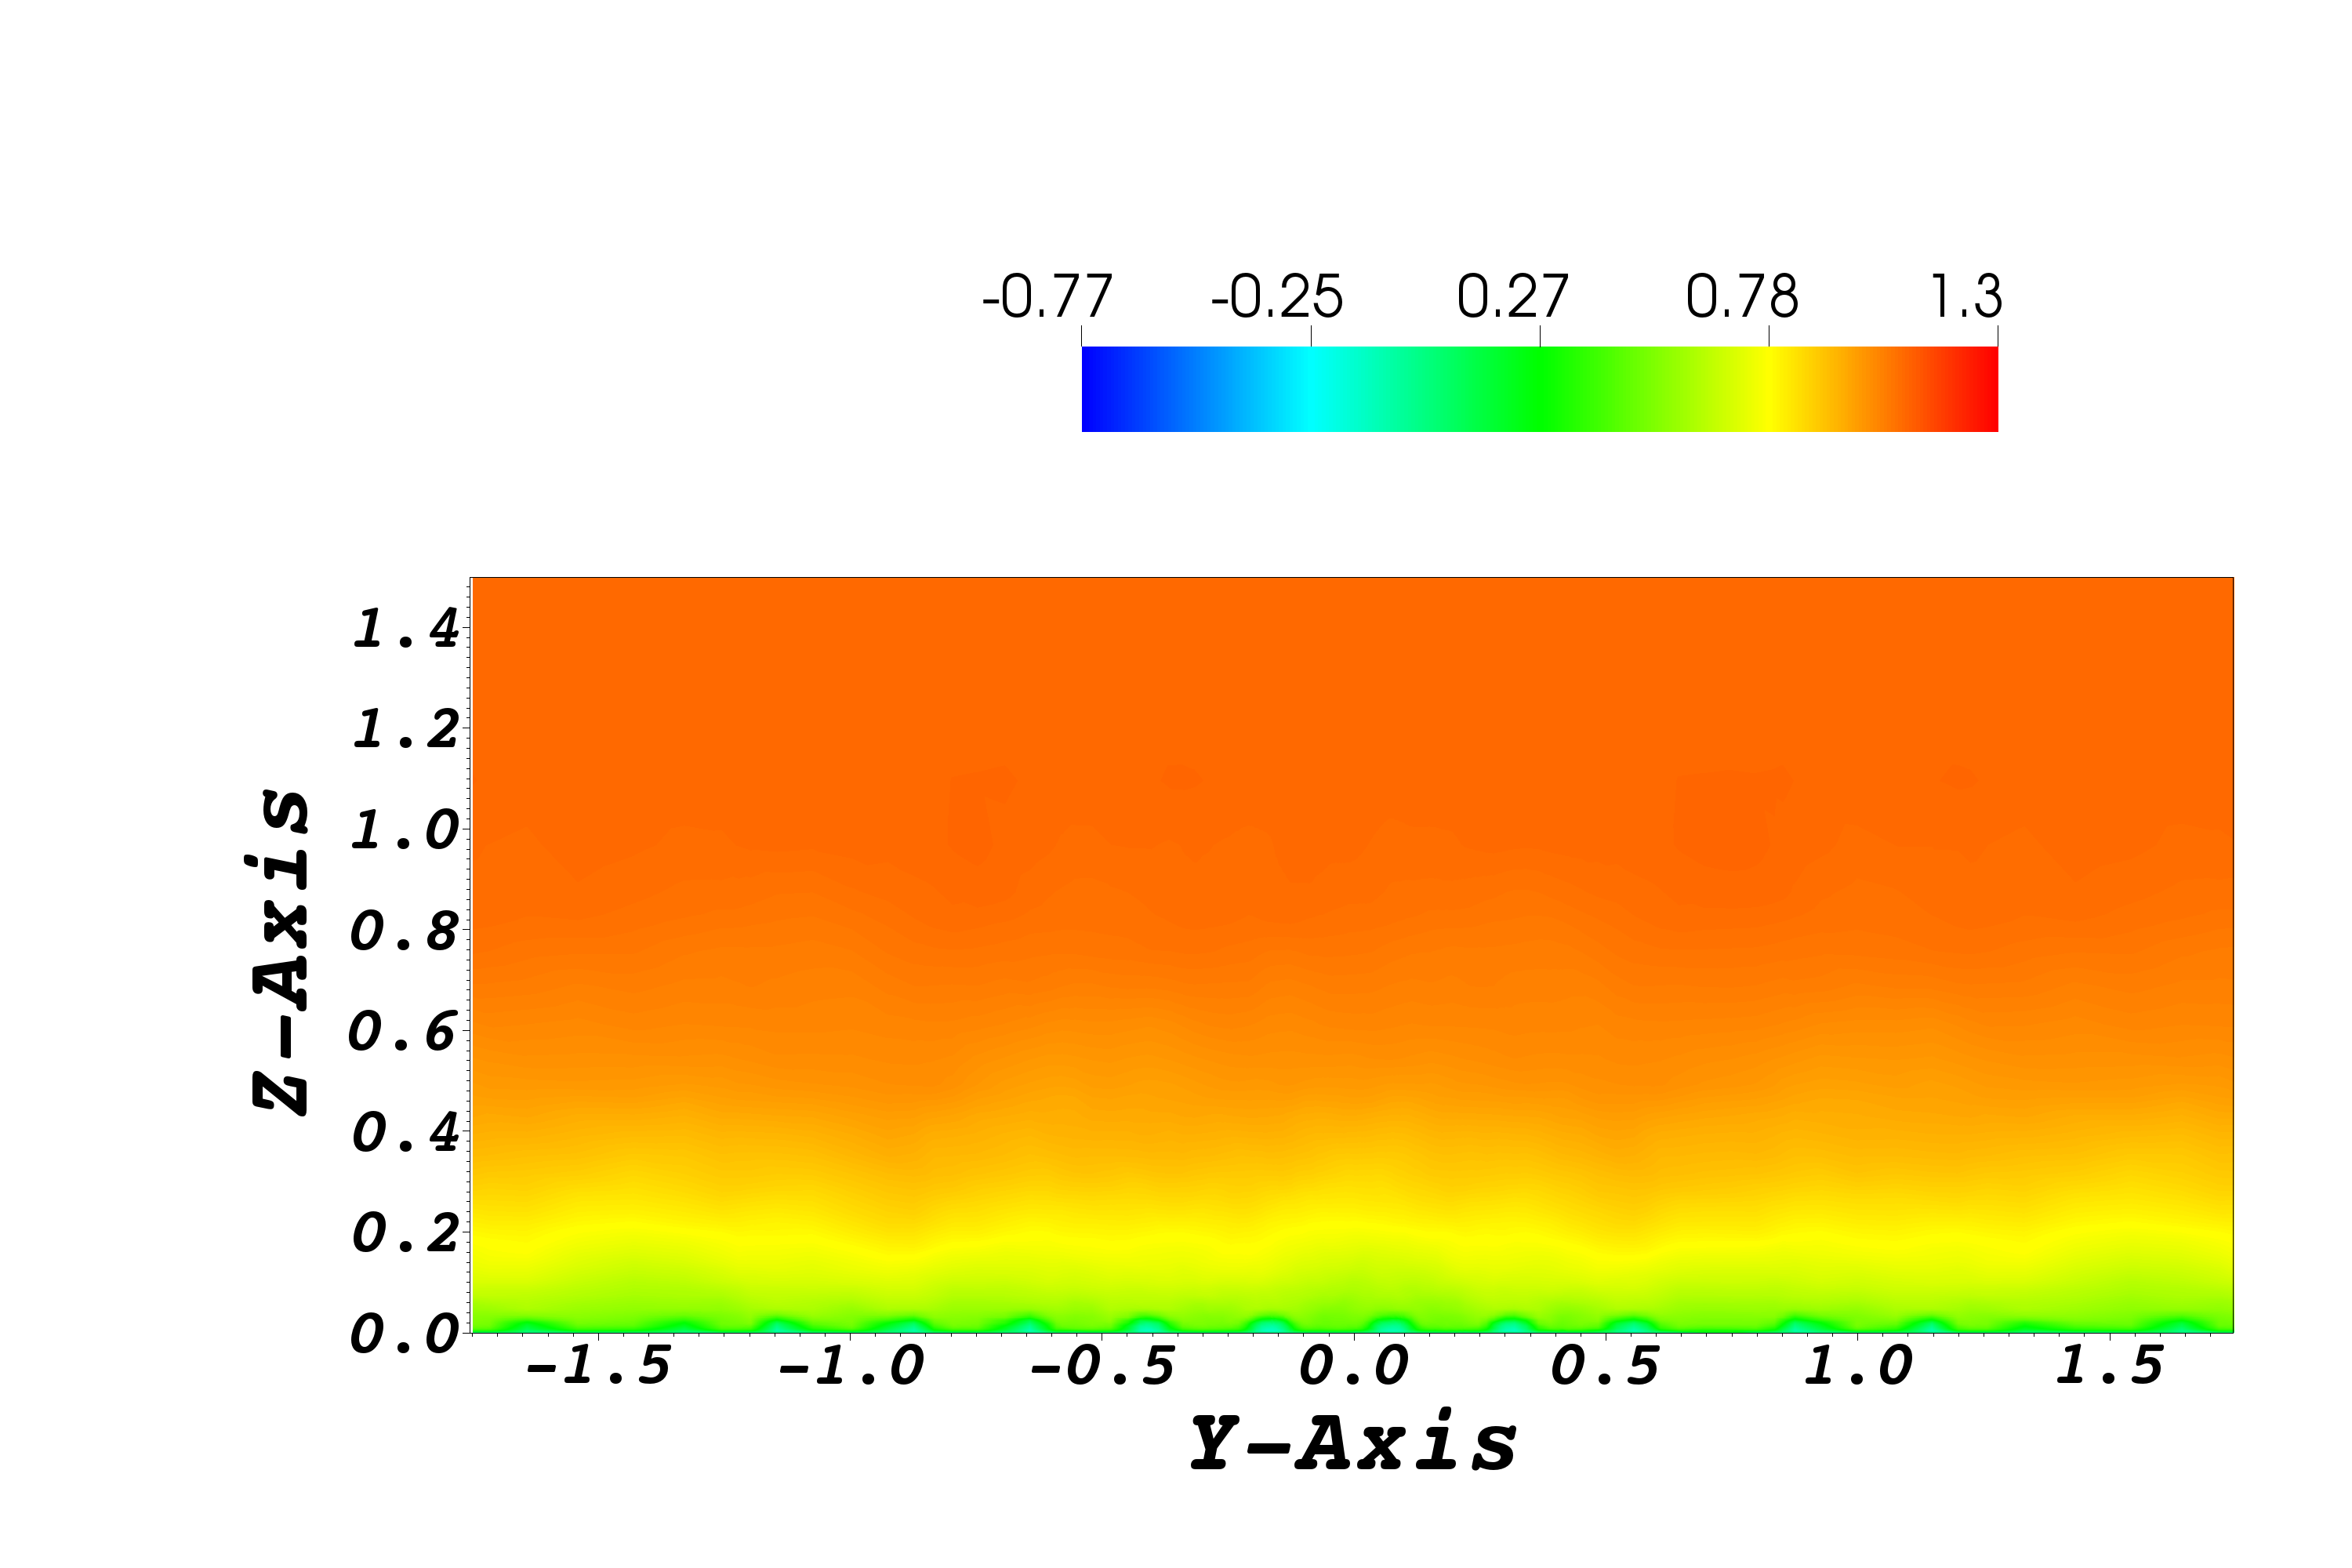
\includegraphics[width=1.0\linewidth]{Figures/inflow_field_avg.png}
  %\captionof{figure}{A figure}
\end{minipage}%
\begin{minipage}{.6\textwidth}
  \centering
  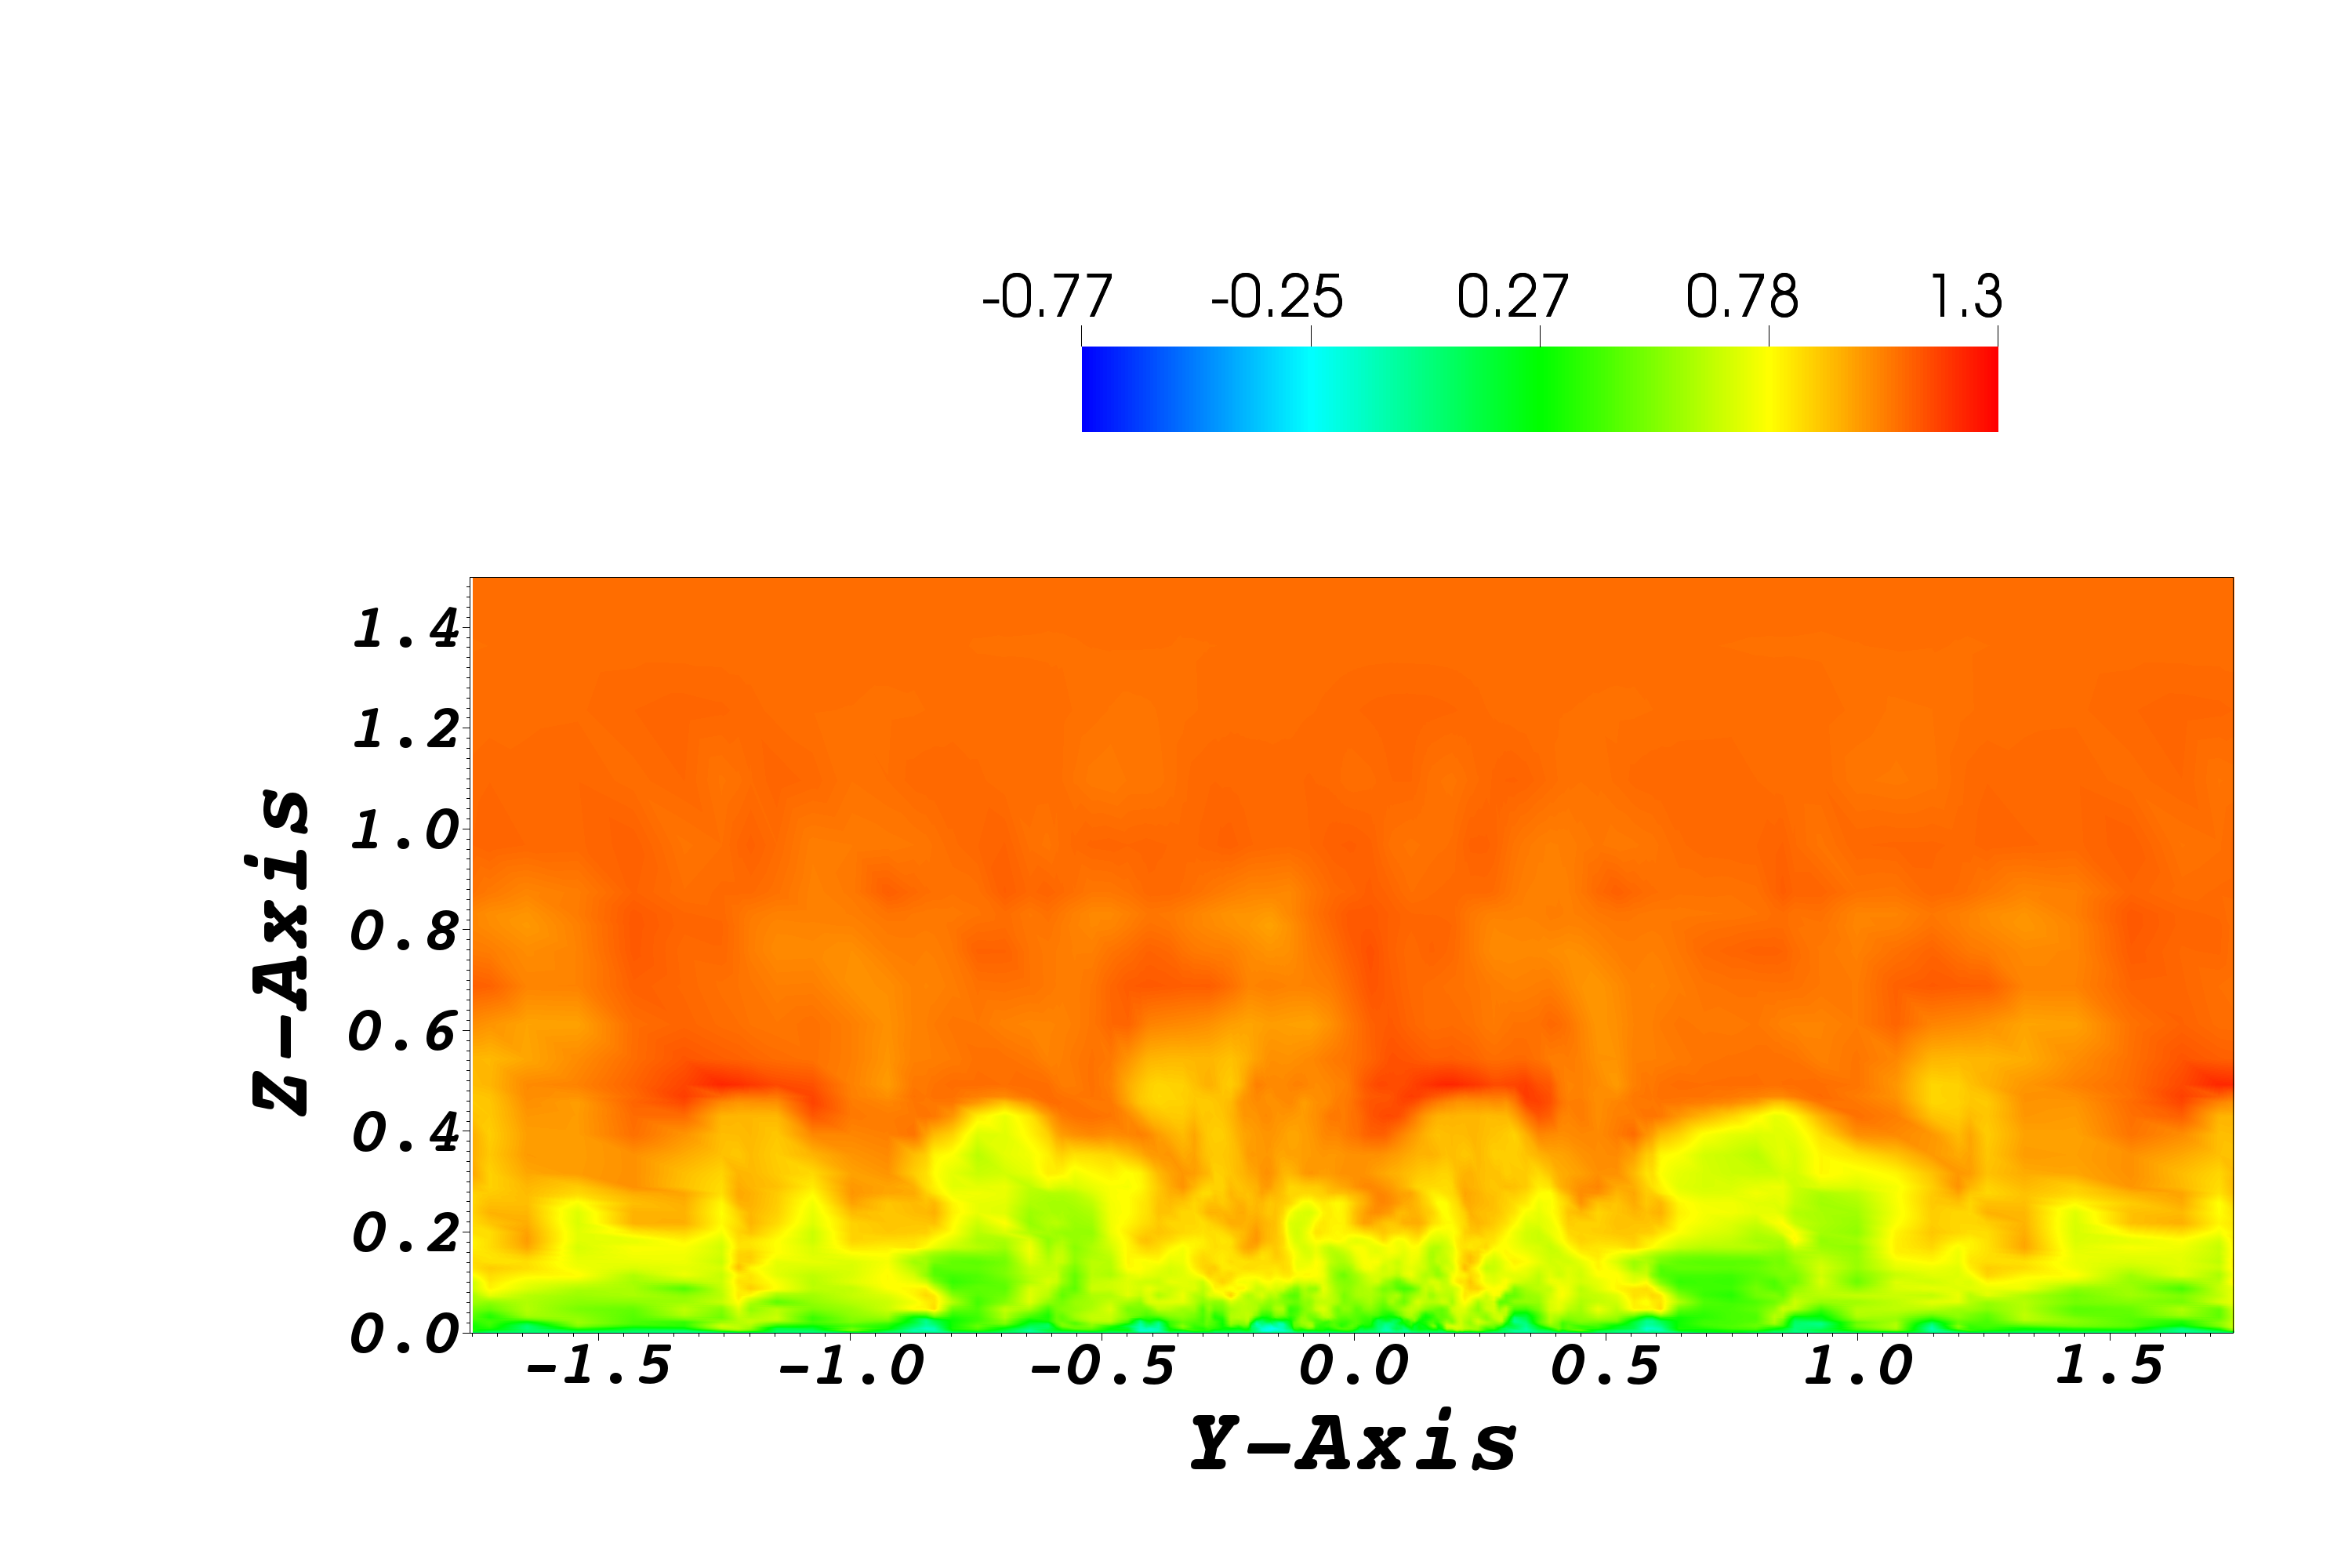
\includegraphics[width=1.0\linewidth]{Figures/inflow_field.png}
\end{minipage}
}
  \caption{The averaged (left) and instantaneous (right) x-velocity on the inflow boundary.}
  \label{fig:inflow}
\end{figure}
%

The simulations in Nek5000 were performed in the following manner; first 6 seconds of initialization of the velocity field in the 
channel, followed by 8 seconds of gas release to initialize the gas-concentration. After assuring that the wind-field was 
correctly created and the released gas had reached the measurement lines furthest from the source the data sampling of 22 seconds 
started.
%
\begin{figure}[h]
	\centering
	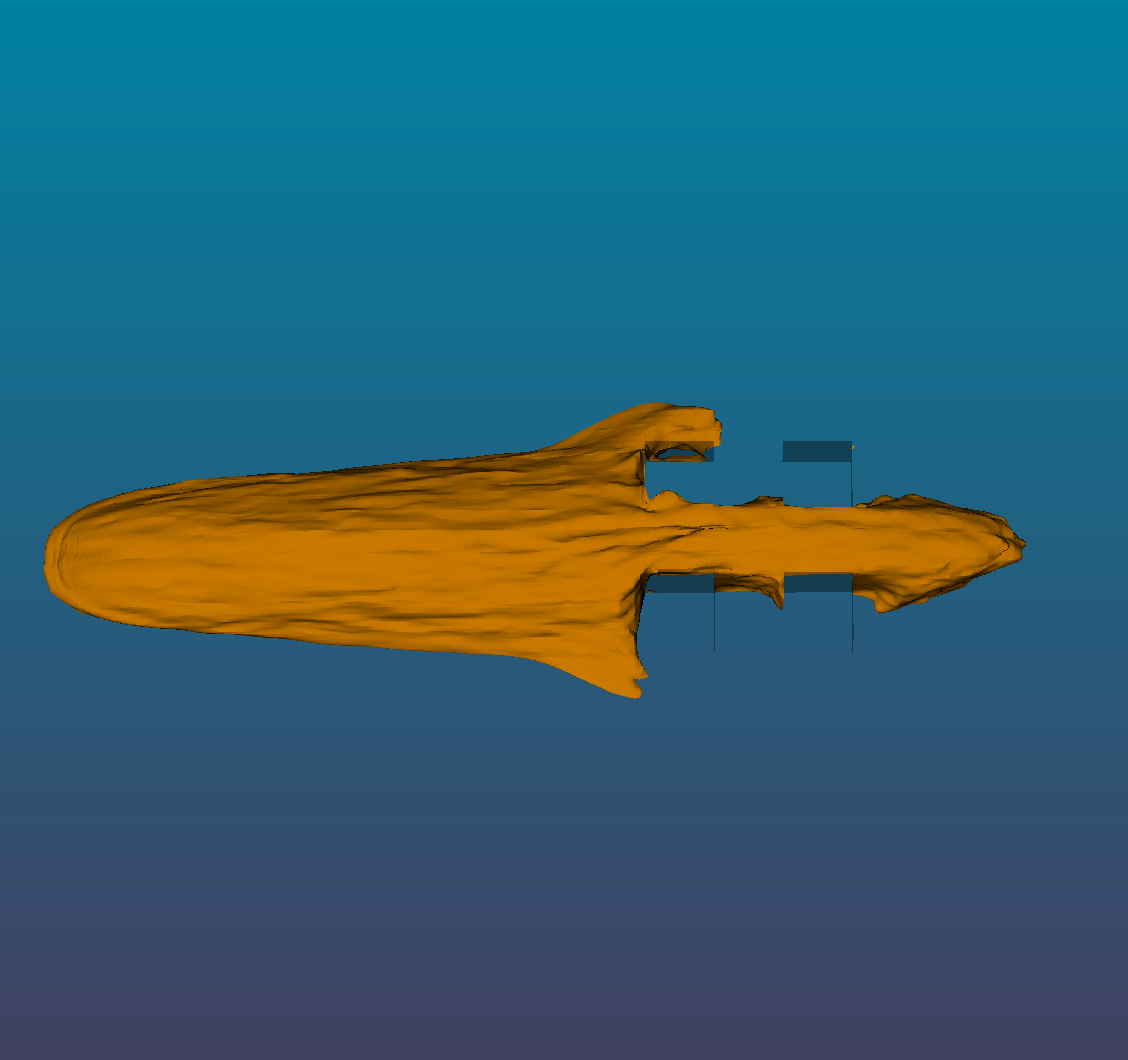
\includegraphics[width=0.6\textwidth]{Figures/plume2.png}
	\caption{An iso-surface of the average concentration with $C=0.03$ 
    after 30 seconds of sampling.}
	\label{fig:plume}
\end{figure}
%

The mesh used in the simulations performed in Nek5000 and the one performed in CDP are 
different, and the resolution in the part of the domain close to the cubes is described 
in~\tref{tab:meshdiff}.
\begin{table}
    \centering
    \begin{tabular}{c| c c c}
        Solver   & $n_x$& $n_y$ & $n_z$ \\ \hline
        CDP      & 28 & 28 & 64 \\ 
        Nek5000  & 22 & 22 & 36 
    \end{tabular}
    \caption{Number of nodes used to represent one cube.}
    \label{tab:meshdiff}
\end{table}

The resolution is better in the simulations done in CDP and especially in 
the $z$-direction. 

\subsection{Results - Gas dispersion} 
This case is a part of a larger project designed to evaluate different solvers 
ability to perform simulations of gas dispersion. The N-S equations are solved using
the $P_NP_N$ formulation with the fractional step method, IOFS with a target Courant number 
equal 2 was enabled to maximize the time step as recommended in~\cite{Nek}. It should be 
mentioned that the stability properties when activating the SGS-model and deactivating the 
filtering was greatly reduced. This effect is captured in~\fref{fig:maxvel} that shows how 
the Smagorinsky model does not damp spurious velocity modes in the same degree as the filter. 
%
\begin{figure}[h]
	\centering
	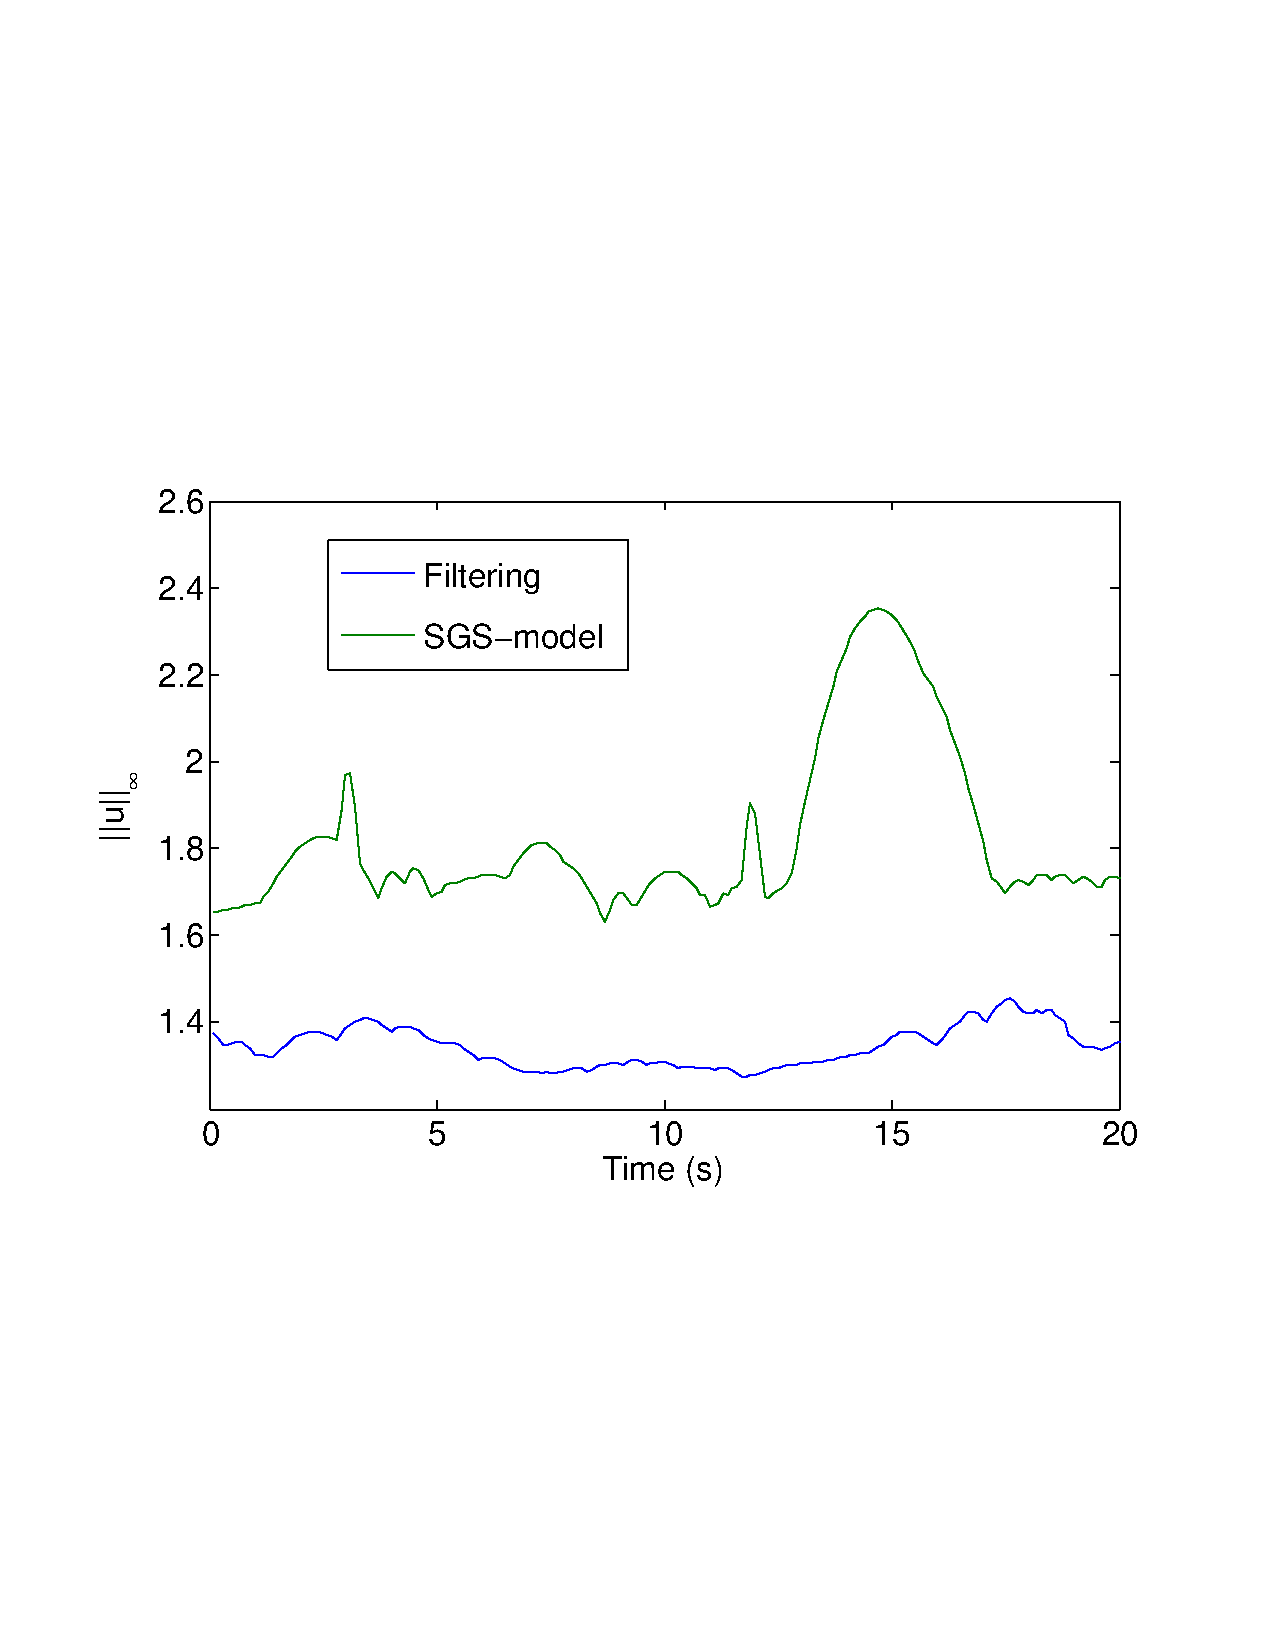
\includegraphics[trim=0.5cm 7cm 0.5cm 7cm, width=0.8\textwidth]{Figures/maxvel.pdf}
    \caption{$||\mathbf{u}||_{\infty}$ as a function of time, the green line represents the 
simulation with the dynamic Smagorinsky SGS-model and the blue line represents the filtering 
with $\alpha = 0.05$ and a quadratic decay on the last 3 modes.}
	\label{fig:maxvel}
\end{figure}
%
%
%\begin{figure}[h]
	%\centering
	%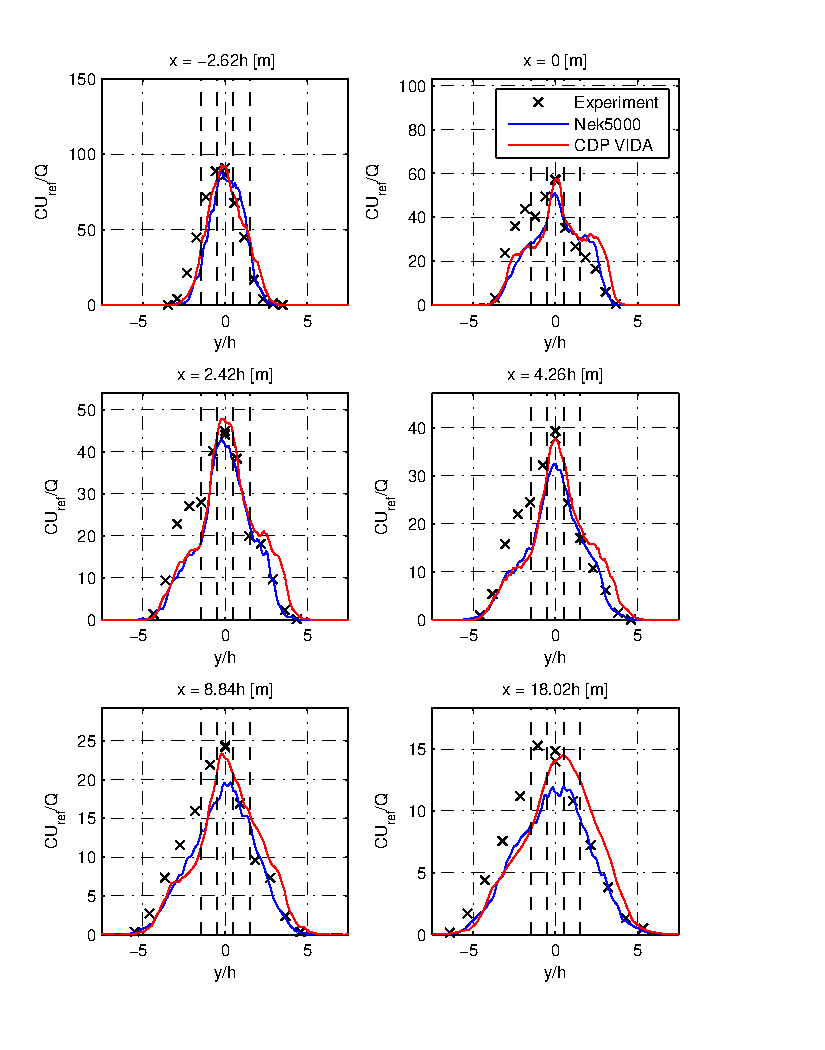
\includegraphics[width=0.8\textwidth]{Figures/NekcH.pdf}
	%\caption{Time-averaged concentration with a sample time of $18.00$ s at $z/H = 0.025$ plotted horizontally and scaled 
	%with the free-stream velocity and emission rate. Compared against wind tunnel data.
%Two dashed lines on either side of the centerline represent the canyon.}
	%\label{fig:cHfilter}
%\end{figure}
%
%
%\begin{figure}[h]
	%\centerline{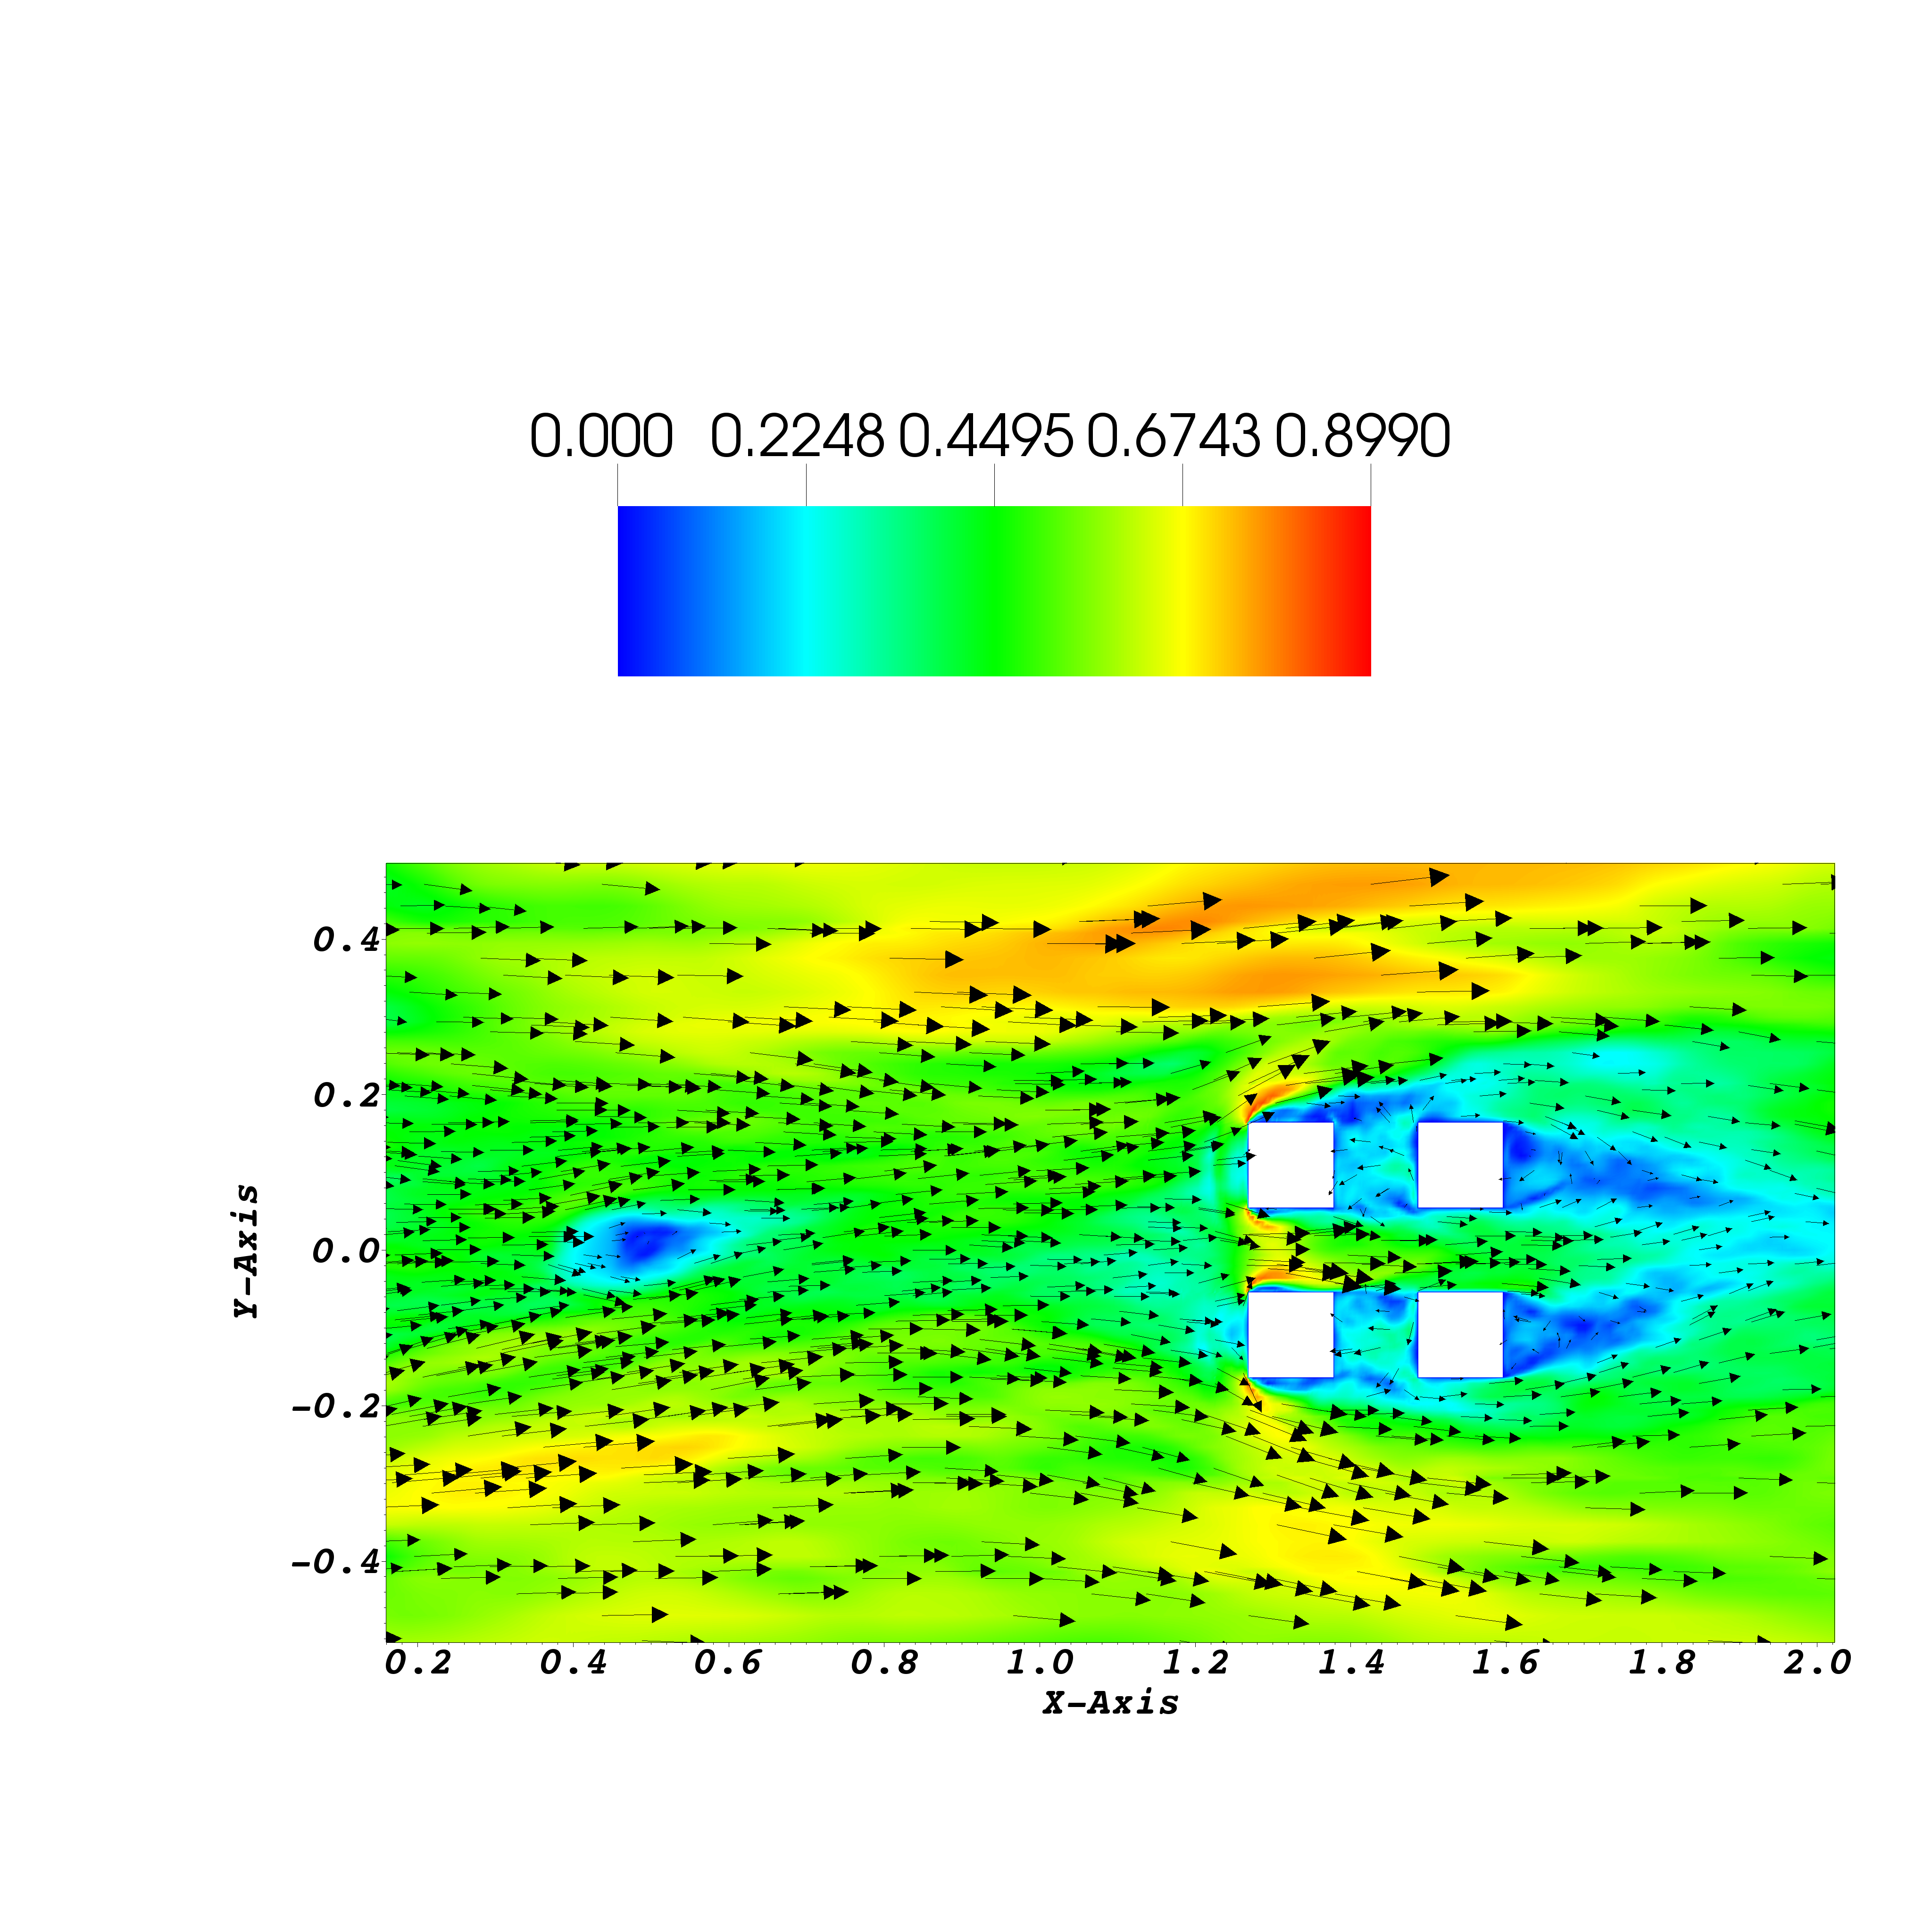
\includegraphics[width=0.8\textwidth]{Figures/vel_field.png}}
	%\caption{velocity field for $z= 0.02$m, around the source and the cubes.}
	%\label{fig:vel_field}
%\end{figure}
%

%\colorbox{green}{redo these simulation in case they were started to early.}
%
%\begin{figure}[h]
	%\centering
	%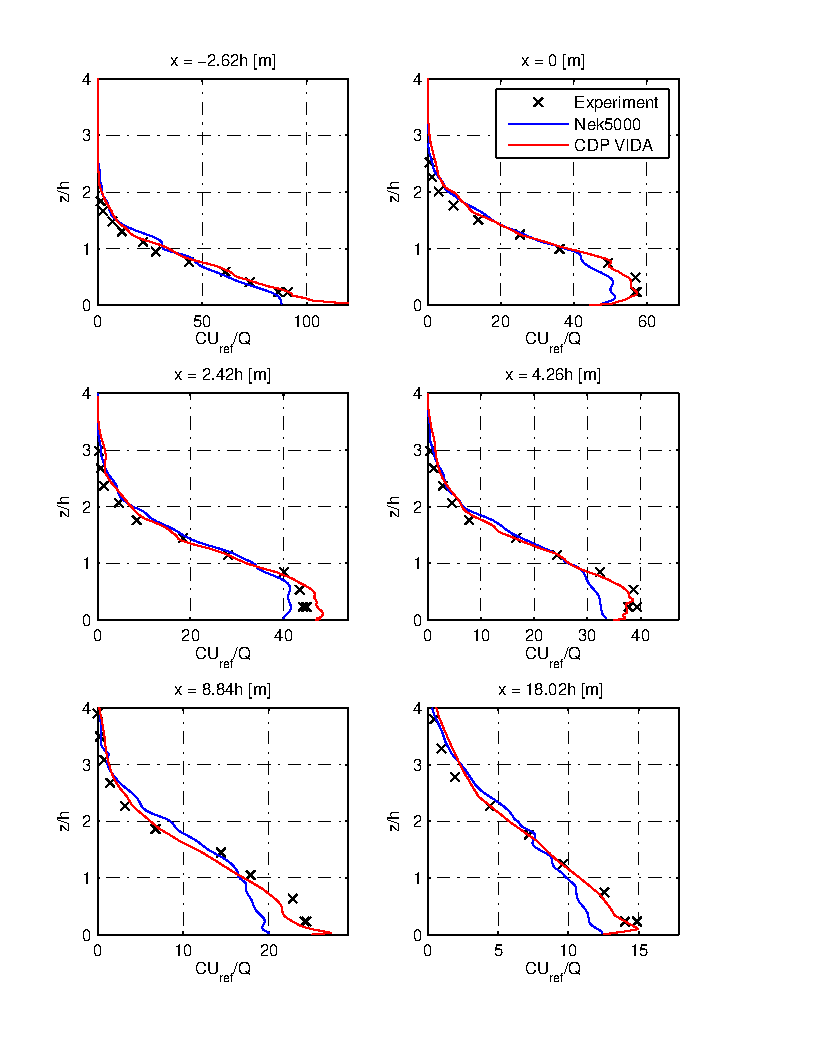
\includegraphics[width=0.8\textwidth]{Figures/NekcV.pdf}
	%\caption{Time-averaged concentration with a sample time of $18.00$ s at $y = 0$ plotted
    %vertically and scaled 
	%with the free-stream velocity and emission rate. Compared against wind tunnel data.
%Two dashed lines on either side of the centerline represent the canyon.}
	%\label{fig:cVfilter}
%\end{figure}
%
%
%\begin{figure}[h]
	%\centering
	%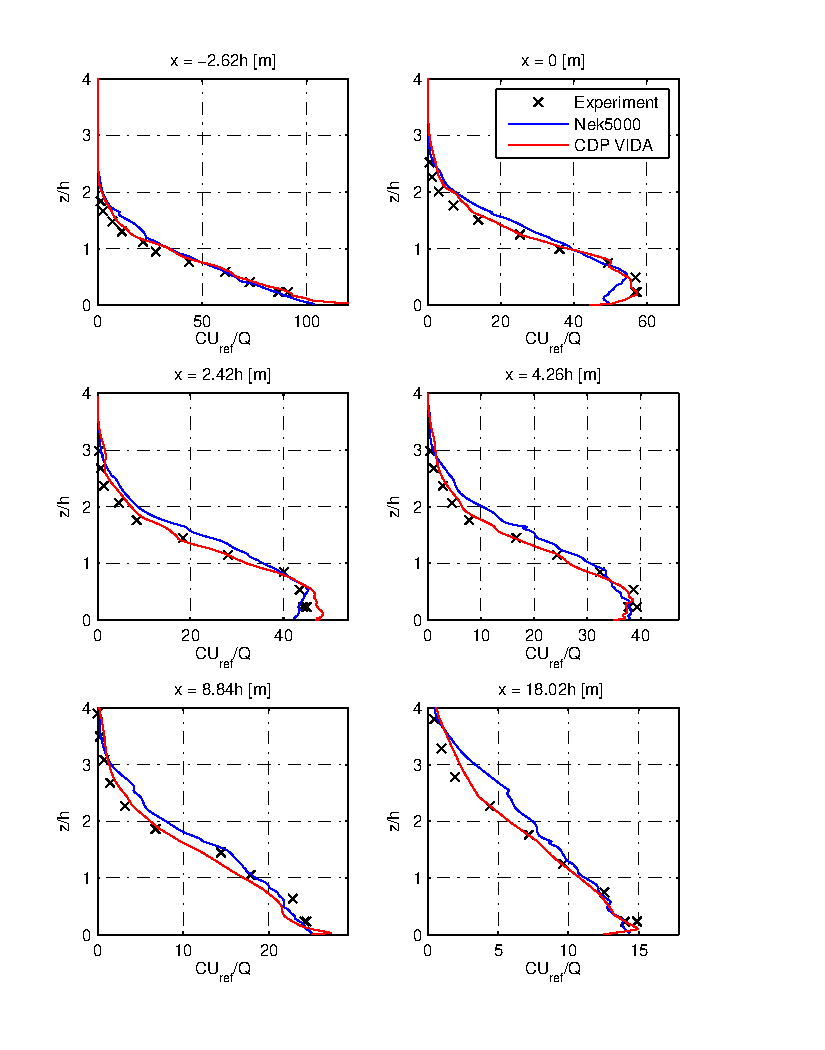
\includegraphics[width=0.8\textwidth]{Figures/Nek_smag_cV.pdf}
	%\caption{Time-averaged concentration with a sample time of $22.00$ s at $y = 0$ plotted
    %vertically and scaled 
	%with the free-stream velocity and emission rate. Compared against wind tunnel data.
%Two dashed lines on either side of the centerline represent the canyon.}
	%\label{fig:cVsmag}
%\end{figure}
%
%
%\begin{figure}[h]
	%\centering
	%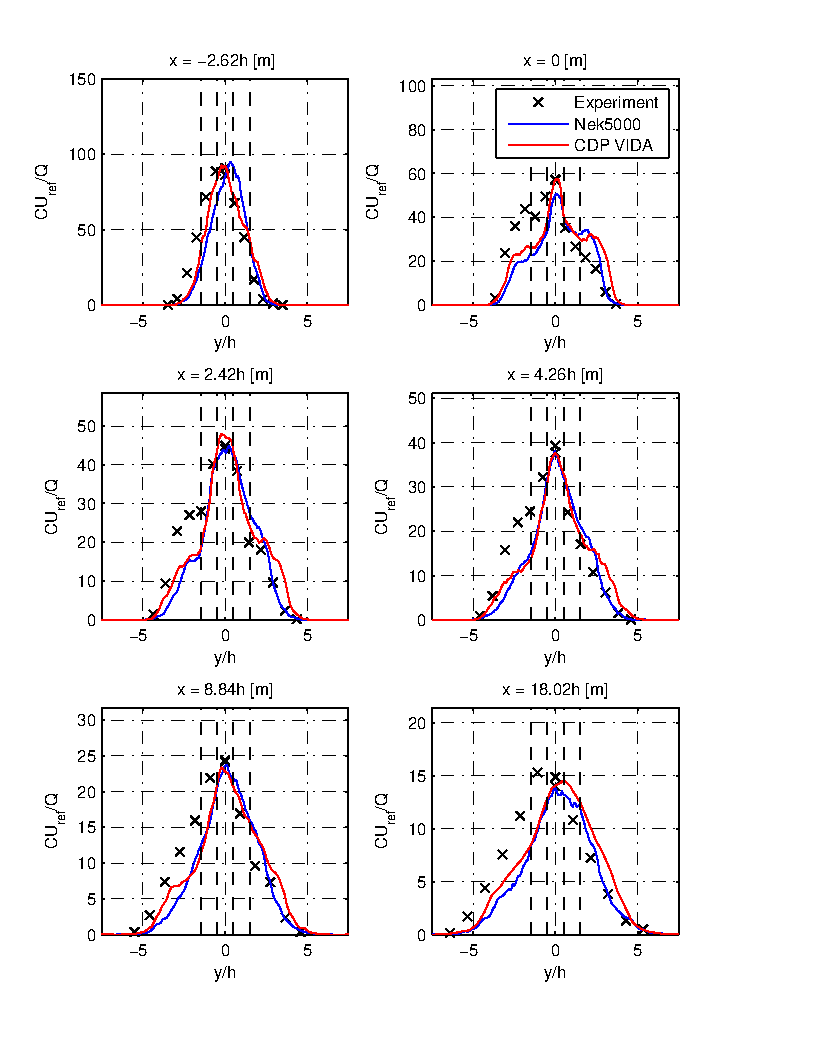
\includegraphics[width=0.8\textwidth]{Figures/Nek_smag_cH.pdf}
	%\caption{Time-averaged concentration with a sample time of $22.00$ s at $y = 0$ plotted
    %vertically and scaled 
	%with the free-stream velocity and emission rate. Compared against wind tunnel data.
%Two dashed lines on either side of the centerline represent the canyon.}
	%\label{fig:cVsmag}
%\end{figure}
%
\newpage
\begin{figure}[h]
    \centering
    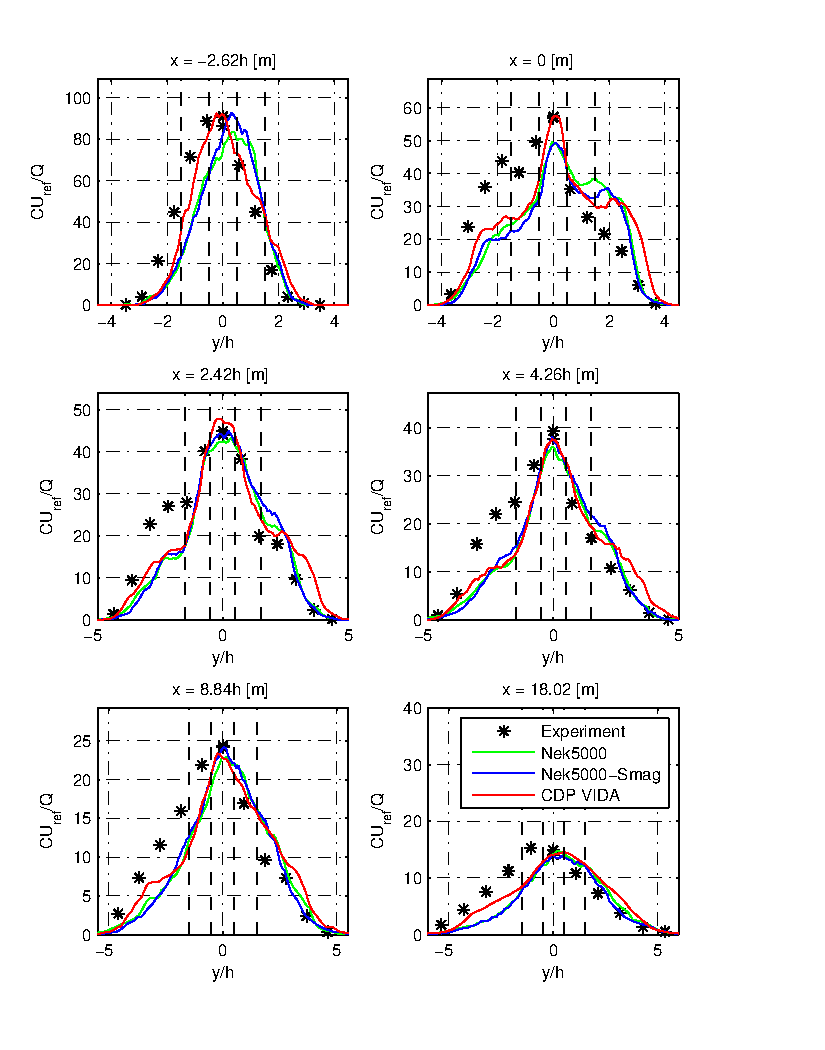
\includegraphics[width=0.9\textwidth]{Figures/NekcH_all.pdf}
    \caption{Time-averaged concentration with a sample time of $22.00$ s at $y = 0$ plotted
    vertically and scaled 
    with the free-stream velocity and emission rate. Compared against wind tunnel data.
Two dashed lines on either side of the centerline represent the canyon.}
    \label{fig:cHall}
\end{figure}

\fref{fig:cHall} shows the scaled concentration along the dotted lines in~\fref{fig:layout}. 
According to this figure Nek5000 does indeed capture the important features of the mean concentration.
At the two first measurement lines the results are slightly skewed to the right, this is to some degree 
also the case for the CDP simulations but not for the experiment. A possible explanation could be that 
the inflow condition favours one of the sides of the domain, or simply that the sampling time is not 
sufficiently long. 
%Along the second measurement line which is placed in the middle of the 4 cubes Nek5000 
%estimates a concentration peak lower than both the reference solutions.  

The results also indicate that the difference between the SGS-model and the filtering
is not that large,
if anything the SGS-model shows a tendency to estimate higher concentration peaks.
In particular the first plot indicates a significant difference.
An important difference between the filtering and the SGS-model is 
that the filter works based on the current state of the flow 
whereas the amount of diffusion added by the SGS-model is mostly decided
by the previous states of the flow.
This could lead to either too much or too little smoothening locally.

\newpage
\begin{figure}[h]
    \centering
    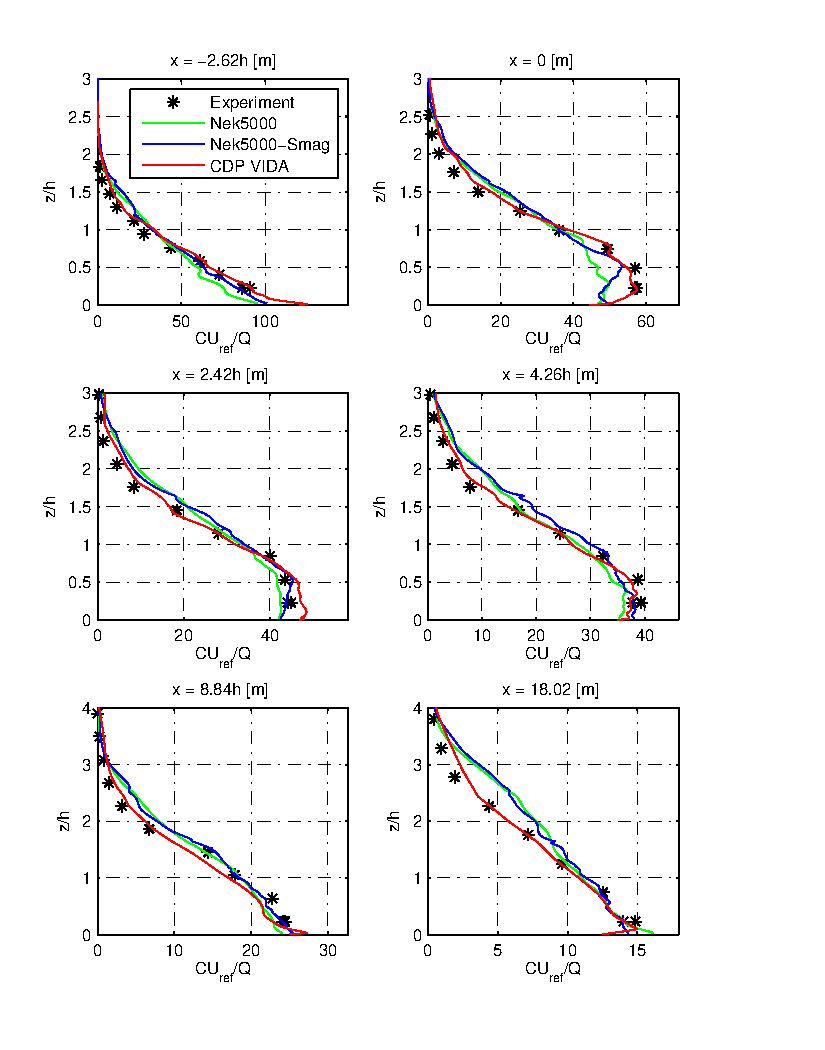
\includegraphics[width=0.9\textwidth]{Figures/NekcV_all.pdf}
    \caption{Time-averaged concentration with a sample time of $22.00$ s at $y = 0$ plotted
    vertically and scaled 
    with the free-stream velocity and emission rate. Compared against wind tunnel data.
Two dashed lines on either side of the centerline represent the canyon.}
    \label{fig:cVall}
\end{figure}
The concentration along the vertical measurement lines is plotted in \fref{fig:cVall} and overall 
Nek5000 provides good results according to the reference solutions. The largest difference is found close 
to the wall right in the middle of the cubes. In particular the simulation with filtering 
underestimates the concentration in this domain. The resolution of the mesh used for the 
Nek5000 simulations in this area is notably worse than for the CDP-simulations.
And in the middle of the cubes neither one of the filter or the Dynamic Smagorinsky model
are able to correct this.
The $P_NP_N$ formulation is known to produce splitting errors of significant sizes 
close to the wall, and could play an important role in this part of the domain.

The simulations were also performed using the $P_NP_{N-2}$ formulation with filtering, and the 
results were similar to those observed above. The SGS-model did however not function at all, 
and resulted in a system crash in one of the earliest time-steps.

As for the performance of Nek5000 the results are baffling. With the same number of processors,
same accuracy criteria, and approximately the same number of nodes in the grid, Nek5000 simulated
one second of flow more than five times as fast as a numerical code comparable to CDP! 
This was done without any particular tuning and with a time-step about $2/3$ of the one used in 
CDP. 


%\begin{figure}[h]
    %\centering
    %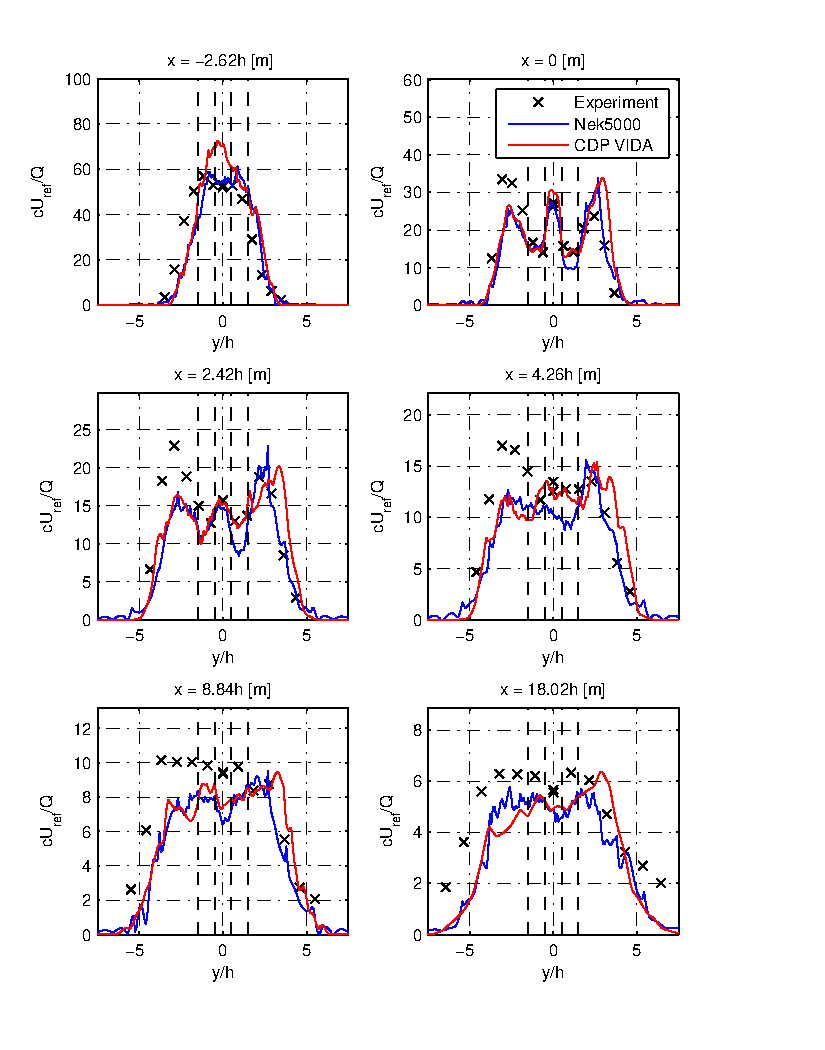
\includegraphics[width=0.8\textwidth]{Figures/Nek_smag_cfluctH.pdf}
    %\caption{Time-averaged concentration with a sample time of $22.00$ s at $y = 0$ plotted
    %vertically and scaled 
    %with the free-stream velocity and emission rate. Compared against wind tunnel data.
%Two dashed lines on either side of the centerline represent the canyon.}
    %\label{fig:cVsmag}
%\end{figure}


\section{Case 2: Drag and lift on a cylinder}
A standard benchmark case for flow solvers is presented in~\cite{benchmark}. 
The case is to calculate the drag and lift coefficients on a cylinder in a rectangular channel.
The setup for the domain and boundary conditions are given in \fref{fig:cylinder}.
The constants applied in the description of the geometry and the coefficient scales are listed 
in table \tref{tab:case2consts}.
%
\begin{table}[h]
    \centering
    \begin{tabular}{c l l}
     Constant & Value & Property \\ \hline
    $H$ & $0.41\text{m}$ & Width and height for the channel \\
    $D$ & $0.1\text{m}$ & Diameter of the cylinder and length scale \\
    $U$ & $0.2\text{m/s}$ & Velocity scale \\
    $\nu$ &  $ 10^{-3}\text{m$^2$/s}$ & Kinematic viscosity of the fluid \\
    $Re$ & $20$ & Reynolds number \\ 
    \end{tabular}
    \caption{Constants for case 2}
    \label{tab:case2consts}
\end{table}
%
Finding the drag and lift coefficient requires a calculation of the velocity field around the cylinder
which is done by solving the unsteady N-S equations until a steady flow is reached. This implies that the
spatial accuracy will dominate the error and one would expect great results in Nek5000 
due to its spectral convergence rate.

The flow is laminar with Reynolds number $Re=20$ so all the 
challenges arising when dealing with turbulent flow does not come to play in this case. 
%
\begin{figure}[h]
    \centering
    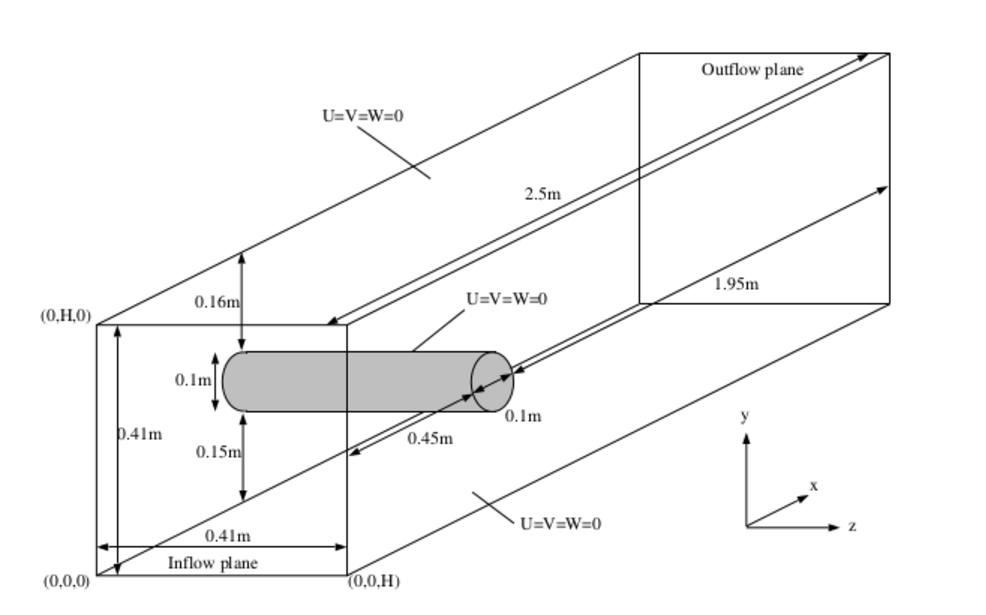
\includegraphics[width = 1.0\textwidth]{Figures/cylinder.pdf}
    \caption{Computational domain and boundary conditions.}
    \label{fig:cylinder}
\end{figure}
%
The drag and lift forces on a surface $S$ are given as 
%
\begin{align}
    F_D = \int_{S}(\rho \nu \frac{\partial v_t}{\partial n}n_y-pn_x)dS, \qquad
    F_L = -\int_{S}(\rho \nu \frac{\partial v_t}{\partial n}n_x+pn_y)dS.
    \label{eq:dragnlift}
\end{align}
%
$v_t$ is the tangential velocity, $\mathbf{n}=[n_x,n_y,0]$ is the unit vector normal to the surface $S$ 
and the tangent velocity vector is defined as $\mathbf{t} = [n_y,-n_x,0]$.
 
Surface integrals in Nek5000 are solved numerically, $\int_S f dS = \sum f_i A_i$, where $f$ is some function and $A_i$ is the area corresponding
to the nodal value $f_i$. $A_i$ corresponds to a two dimensional mass matrix in Nek5000 available for all elements.

The coefficients corresponding to these forces known as the drag and lift coefficients 
are given by the formulas 
\begin{align}
    c_D = \frac{2F_D}{\rho U^2 D H}
    \qquad , \qquad
    c_L = \frac{2F_L}{\rho U^2 D H}.
    \label{eq:dragnliftcoeffs}
\end{align}


Nek5000 provides functions for calculating lift and drag on any user-specified object.
The function is called \verb|drag_calc(scale)|, with the input parameter 
defined by the user, for this case \verb|scale| $=2/(\rho U^2DH)$.  
Apart from this the function \verb|set_obj()| has to be modified to create an object 
that consists of pointers to all the faces on the cylinder.
%Let $x,y$ be points in the computational domain, $x_c,y_c$ be the coordinates to the 
%center line in the cylinder and $0<tol\ll1$ be some user defined tolerance. The faces that belong to the cylinder can then be found by 
%looping over all elements and their faces evaluating $\epsilon = \sqrt{(x-x_c)^2+(y-y_c)}$.
%If $\epsilon < tol$ for an entire face then this face is known to 
%belong to the cylinder and is added to the object. Nek also allows the user to specify multiple objects 
%assigning the faces of interest to object 1, object 2 etc. The geometry and mesh 
%for this case was generated in ICEM, and the total number of elements are 2070. 
%For the final calculation polynomial degree $P = 11$ was applied leading to a 
%total of $N = 2755170$.
%
\begin{figure}[h]
    \centering
    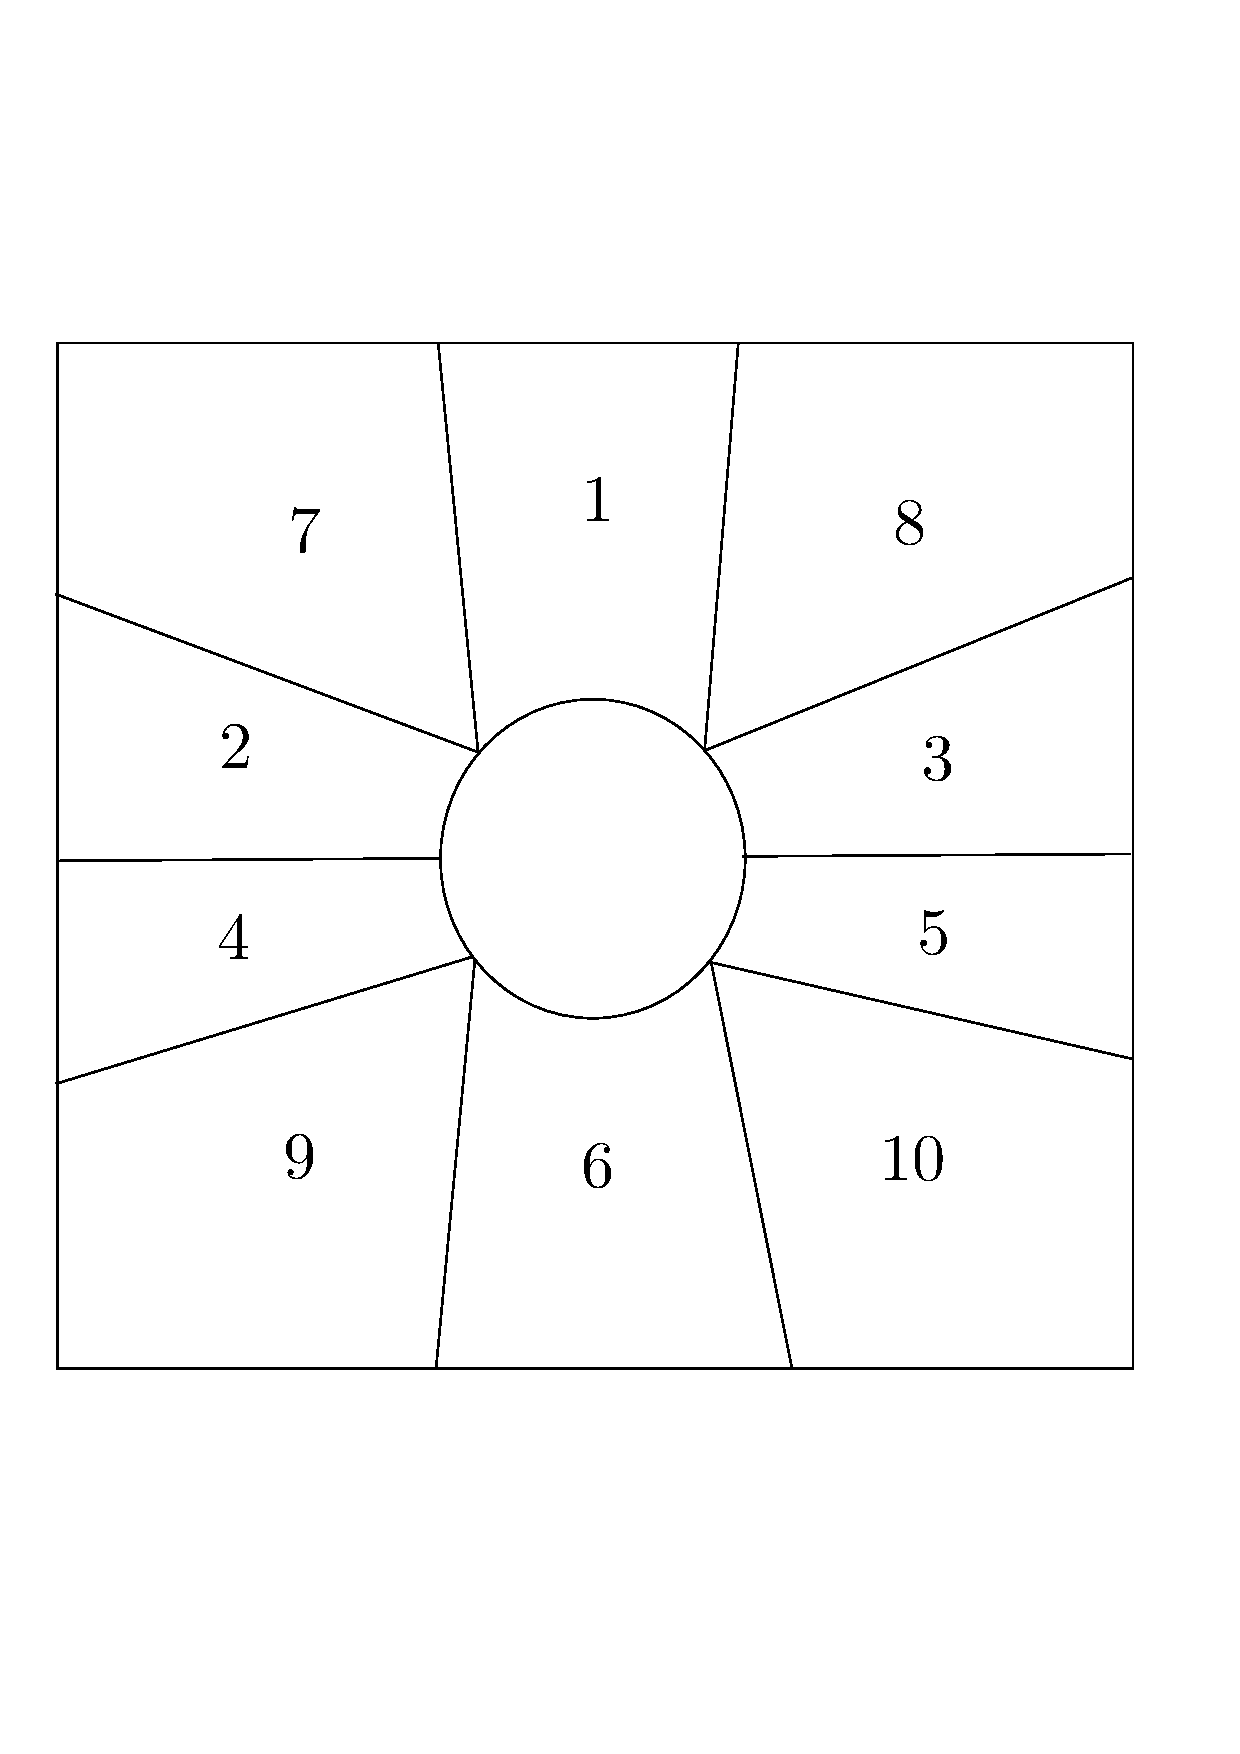
\includegraphics[width = 0.3\textwidth]{Figures/cyl_elem.pdf}
    \caption{Initial mesh around cylinder.}
    \label{fig:cyl_elem}
\end{figure}
%
The mesh around the cylinder is illustrated in \fref{fig:cyl_elem}.
Initially this case was solved using a second degree polynomial to describe the circle segments
corresponding to each element. However with the new routine implemented as described 
in~\cref{xyzarc} the circle segments could be represented with the same order as 
the polynomials used for the velocity space. The importance of the error resulting 
from the second degree approximation of the circle segments is presented in \cref{results}.
%Note that these elements was split in three, in order to obtain 
%a finer mesh in the region of interest. Of the elements numbered in~\fref{fig:cyl_elem}
%only the first six contains edges on the cylinder.Hence the second order polynomials 
%describing the curved edges describe approximately $\Theta = 360^{\circ}/(6\cdot 3) = 20^{\circ}$
%of the complete circle. 

An additional test that is performed on this case is how different settings in Nek5000 will affect the estimation of the drag and lift coefficients.
Perhaps most curious is whether the $P_NP_N$ or $P_NP_{N-2}$ formulation is applied. Note that the pressure in the latter formulation is 
not defined on the boundary of the cylinder and does therefore need to be extrapolated onto the surface in order for the integral to be 
calculated. On the other side is the splitting scheme implied by the $P_NP_N$ forces the erroneous boundary condition on the pressure.
%
\subsection{Results - benchmark comparison}
The effect of the algorithm explained in \cref{xyzarc} is
illustrated by solving a laminar flow test problem. 
The solution is compared with previously benchmark computations performed by a number of 
contributors~\cite{benchmark}. 

The results are presented in \tref{tab:testcase}, and they confirm that the treatment of the geometry is 
essential, both coefficients are computed with significantly better accuracy. 
%
\begin{table}[h]
\centering
\begin{tabular}{l l c c c c}
		\toprule
		\# of Cells & Software & $c_D$ & $c_L$ & \%\textbf{Err} $c_D$ &\%\textbf{Err} $c_L$ \\ \midrule 
		2124030& Nek5000 (mid) & 6.18349 & 0.008939 & 0.030 & 4.19 \\ 
		2124030& Nek5000 (arc) & 6.18498 & 0.009413 & 0.006 & 0.13 \\
		3145728 & CFX 		 & 6.18287 & 0.009387 & 0.04 &0.15 \\
		3145728 & OF	     & 6.18931 & 0.00973 & 0.06 &3.5 \\
		3145728 & FEATFLOW   & 6.18465 & 0.009397 & 0.01 &0.05 \\
		\bottomrule	
	\end{tabular}
	\caption{Results for the drag and lift coefficients with reference values 
	$c_D = 6.18533$ and $c_L = 0.009401$. $p=11$ for the simulations in Nek5000.}
\label{tab:testcase}
\end{table}
%
Compared with the results from the other softwares applied in~\cite{benchmark} Nek5000 performs 
just as well or better in most cases. It should be mentioned that the division of the grid is created
in a different manner for Nek5000 so the comparison is not as direct as it may seem from the table.

\subsection{Results - internal adjustments }
As discussed in \cref{nek} there are many adjustments available in Nek5000. 
To enlighten the actual effect on the results, several different settings were 
investigated for this case and the results are presented in \tref{tab:perf}. 
The spectral convergence is also confirmed in \fref{fig:liftconv} by calculating the 
lift coefficient error for increasing polynomial degree. 
%
\begin{figure}[h]
	\centerline{
        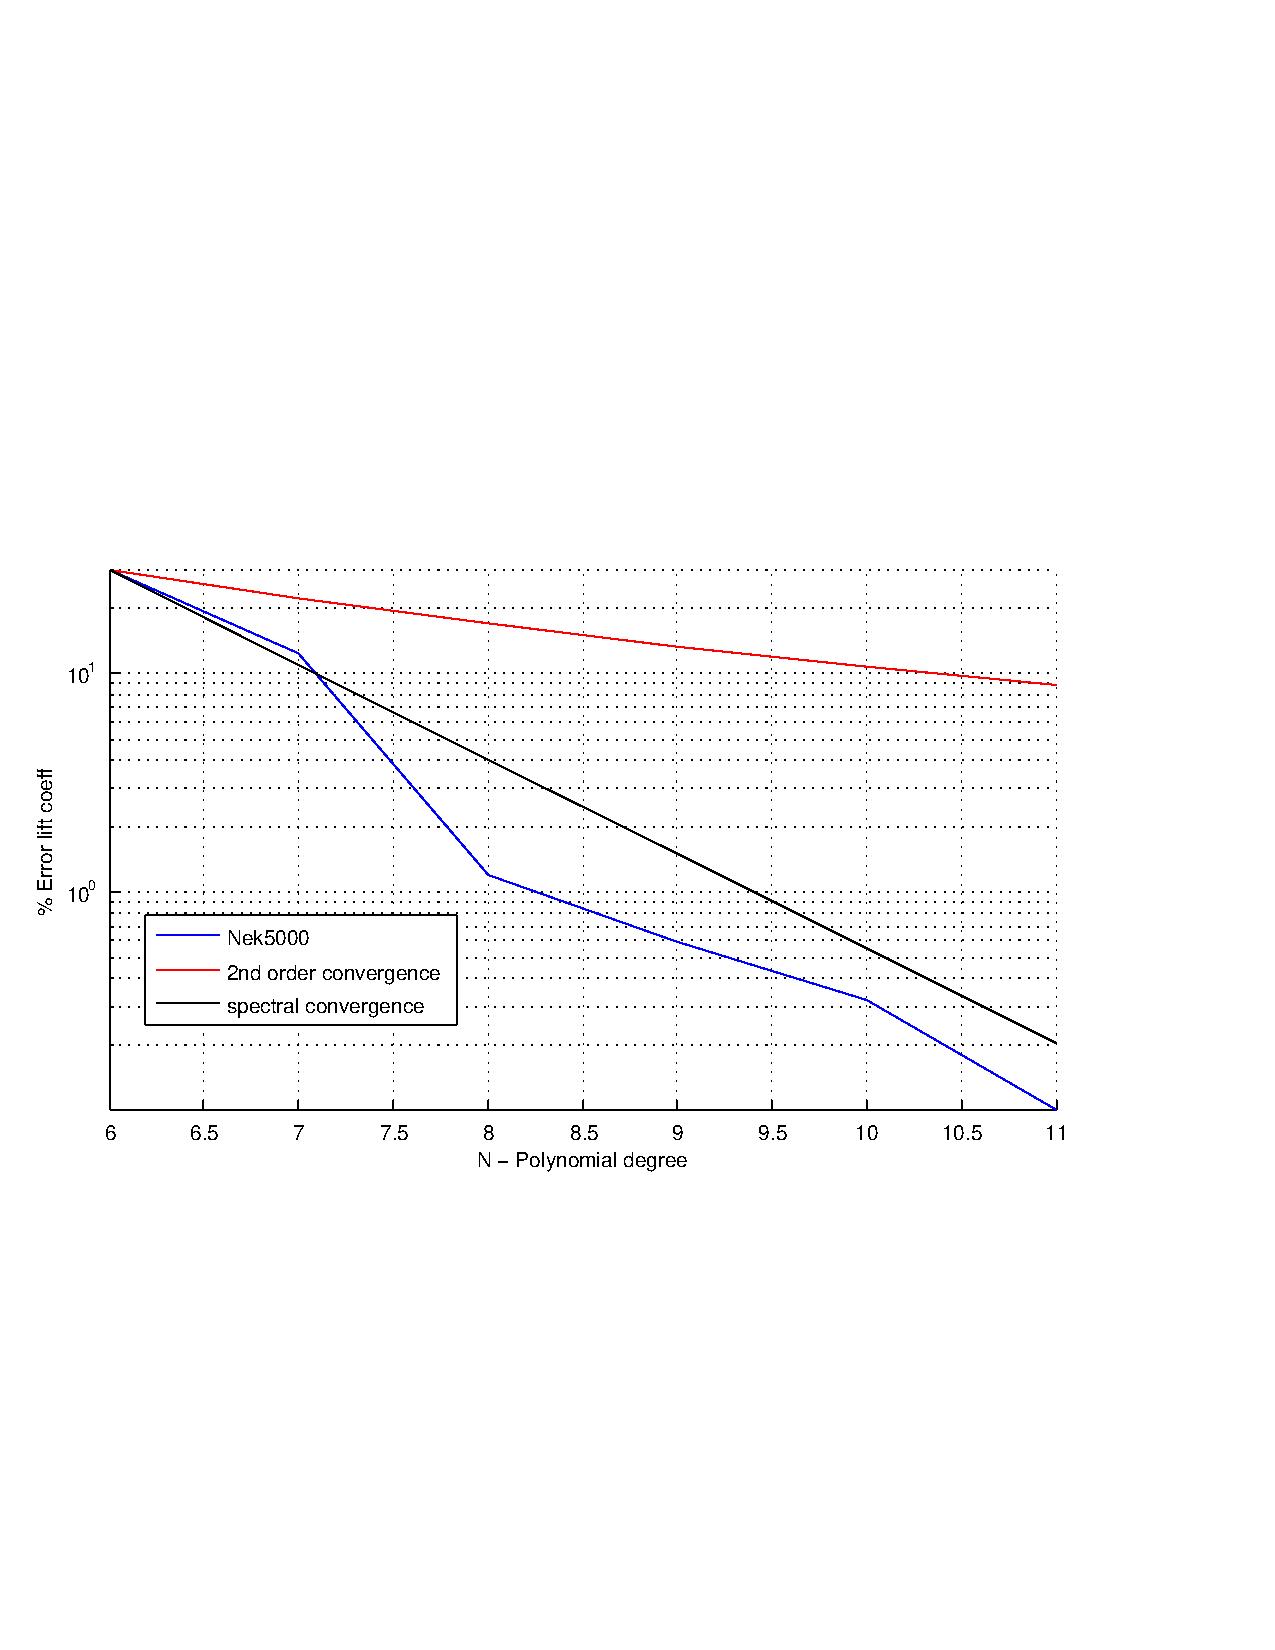
\includegraphics[trim=0.5cm 7cm 0.5cm 7cm, width=0.8\textwidth]{Figures/lift_coef4.pdf}}
	\caption{The logarithm of the error plotted against the polynomial degree. All results 
        are with $P_NP_{N-2}$ and dealiasing, and they are solved without using the 
    characteristic scheme or any filtering. A line illustrating a second order convergence is 
    plotted to illustrate the convergence rate.}
	\label{fig:liftconv}
\end{figure}
%

The setting that has the biggest impact on the result is the $P_NP_N$ scheme which clearly performs 
worse than the others. This is as expected since the discrete splitting is known to converge faster
for steady state flows. Notice however that by reducing the time-step the effect of the algebraic splitting
greatly reduces and achieves results of similar order as the discrete splitting.
Use of the IOFS method also has a negative effect on the accuracy,
this is also as expected because of the stability-accuracy trade-off for this method.
Remember that this scheme allows a much higher time step. The filtering is the least significant change
which confirms the analytical results from \eref{eq:filterenergy}. 
%
\begin{table}[h]
    \centering
    \begin{tabular}{c | c c c c c | c c }
         & \multicolumn{5}{|c|}{Settings} & \multicolumn{2}{|c}{\% Error} \\\hline
         \# & $\Delta t$ & ifsplit & Dealiasing & IOFS & Filter & $c_D$ & $c_L$ \\  \hline 
         1 & 6e-4& No & Yes& No & No & 0.005 & 0.10\\
         2 & 6e-4& No & Yes& No & Yes& 0.005 & 0.43\\
         3 & 6e-4& No & Yes& Yes& No & 0.005 & 0.18\\
         4 & 6e-4& No & No & No & No & 0.005 & 0.03\\
         5 & 6e-4& Yes& Yes& No & No & 0.012 & 2.35\\
         %6 & 4.5e-4& Yes& Yes& No & No & 0.015 & 0.01\\
         %7 & 3e-4& Yes& Yes& No & No & 0.018 & 0.01\\
    \end{tabular}
    %\begin{tabular}{c | c c c c | c c | c c c}
         %& \multicolumn{4}{|c|}{Settings} & \multicolumn{2}{|c|}{\% Error} & \multicolumn{3}{|c}{Data} \\\hline
         %\#  & ifsplit & Dealiasing & IOFS & Filter & $c_D$ & $c_L$ & DT & CFL & T/Tstep \\ \hline 
         %1 & F & T & F & F & 0.005 & 0.102 & 1e-04 & 2.03 & 2.1e-02 \\
         %2 & T & T & F & F & 0.013 & 2.349 & 1e-04 & 2.03 & 2.1e-02 \\
         %3 & F & T & F & T & 0.005 & 0.431 & 1e-04 & 2.03 & 2.1e-02 \\
         %4 & F & T & T & F & 0.005 & 0.179 & 1e-04 & 2.03 & 2.1e-02 \\
         %5 & F & F & F & F & NaN   & NaN   & 1e-04 & 2.03 & 2.1e-02 \\
    %\end{tabular}
    \caption{Test of solver settings in Nek5000.}
    \label{tab:perf}
\end{table}
%

Be aware that these results are obtained from a laminar test case and does not in any way 
suggest any optimal adjustment for Nek5000. An important example of this is the fact that 
deactivating de-aliasing yields better results. For a coarser mesh or a more turbulent flow 
this would not be the case, and that the result is better is probably due to 
the accuracy, which are close to the accuracy given by the reference solution. 
The resuslts do however give an indication to the general effect of these settings that 
are worth noticing.

%----------------------------------------------------------------------------------------
\chapter{Concluding remarks}
Nek5000 has proven to give accurate results with a relatively coarse mesh as
presented in~\cref{results}. This is as expected since it is based on a higher order 
method known to yield great accuracy. As for the performance it is no doubt that the 
efforts put into the efficiency of the code has paid off. The possibility to obtain 
results 5-10 times faster than similar softwares is an important factor to keep in mind. 
The polynomial degree is chosen by changing a single parameter, which makes performance tests
and accuracy adjustments simple to do. 

Since the mathematical formulation in Nek5000 is based on a tensor product of the basis functions 
in each direction it is limited to the use of hex-mesh. This is no problem for the geometries 
studied in this thesis, but for complex geometry the use of tetrahedral mesh is mandatory.
It did also prove difficult to work with refinements made in ICEM which restricts the possibility 
to make a mesh with large differences in grid size.

Another aspect worth noticing is the filtering procedure which has some similarities to variational multiscale
as presented in~\cref{physfilt}. It would be interesting to design some test cases to further 
investigate its properties. 

The fact that Nek5000 is an open-source code is also a huge advantage to other black-box solvers. 
Although the user community is not that large there are several commited users that provide 
their help on short notice. Many different examples are available, and the user guide 
contains a nice introduction with everything needed to get the program up and running. 
The documentation of variables and functions are sometimes missing, which is the main motivation 
to create Appendix~\ref{AppendixB}. 


\section{Further work}
The surface projection could be expanded and improved in many ways. Making it iterative 
to make sure the GLL-points are distributed correspondingly, The norm corresponding
to the normal is prone to give errors and should be calculated based on points further away\ldots.
For the simple array case it was experimented with different meshes and the refinement procedure 
in ICEM quickly leads to small elements with wide angles which tends to lead to problems 
in Nek5000. The author do however believe that by making an ogrid around the most important part of 
the domain, say for instance the box, $x/H < 3,\: |y|/H < 0.4,\: z/H < 0.15$ the nodes could have been 
distributed in a more economical fashion and an overall better result could have been achieved.


\colorbox{green}{How did Nek5000 perform overall, user-friendly ?,correctness,speed etc.}

 
%\input{Chapters/Chapter5} 
%\input{Chapters/Chapter6} 
%\input{Chapters/Chapter7} 

%----------------------------------------------------------------------------------------
%	THESIS CONTENT - APPENDICES
%----------------------------------------------------------------------------------------

\addtocontents{toc}{\vspace{2em}} % Add a gap in the Contents, for aesthetics

\appendix % Cue to tell LaTeX that the following 'chapters' are Appendices

%% Include the appendices of the thesis as separate files from the Appendices folder
%% Uncomment the lines as you write the Appendices

% Appendix A

\chapter{Fundamental basics of numerical analysis} % Main appendix title

\label{AppendixA} % For referencing this appendix elsewhere, use \ref{AppendixA}

\lhead{Appendix A. \emph{Numerical analysis}} % This is for the header on each page - perhaps a shortened title

\section{GLL-quadrature}
\section{Essential polynomials}
\begin{enumerate}
    \item Legendre polynomials
    \item Lagrange basis 
\end{enumerate}

\section{Preliminary concepts}

\begin{enumerate}
    \item coersiveness
    \item Bounded  
\end{enumerate}

\section{Lax-Milgram theorem}

Stating the theroem without proof 


% Appendix Template

\chapter{Variables and Functions in Nek5000} % Main appendix title

\label{AppendixB} % Change X to a consecutive letter; for referencing this appendix elsewhere, use \ref{AppendixX}

\lhead{Appendix B. \emph{Variables and functions in Nek}} % Change X to a consecutive letter; this is for the header on each page - perhaps a shortened title

\section{Variables}

\section{Functions}

%%\input{Appendices/AppendixC}

\addtocontents{toc}{\vspace{2em}} % Add a gap in the Contents, for aesthetics

\backmatter

%----------------------------------------------------------------------------------------
%	BIBLIOGRAPHY
%----------------------------------------------------------------------------------------

\label{Bibliography}

\lhead{\emph{Bibliography}} % Change the page header to say "Bibliography"

\bibliographystyle{unsrtnat} % Use the "unsrtnat" BibTeX style for formatting the Bibliography

\bibliography{Bibliography} % The references (bibliography) information are stored in the file named "Bibliography.bib"

\end{document}  
